%--------------------
% Packages
% -------------------
%\documentclass[11pt,a4paper]{article}
%\usepackage[utf8x]{inputenc}
%\usepackage[T1]{fontenc}
%%\usepackage{gentium}
%\usepackage{mathptmx} % Use Times Font
%%
%
%\usepackage[pdftex]{graphicx} % Required for including pictures
%\usepackage[swedish]{babel} % Swedish translations
%\usepackage[pdftex,linkcolor=black,pdfborder={0 0 0}]{hyperref} % Format links for pdf
%\usepackage{calc} % To reset the counter in the document after title page
%\usepackage{enumitem} % Includes lists
%
%\frenchspacing % No double spacing between sentences
%\linespread{1.2} % Set linespace
%\usepackage[a4paper, lmargin=0.1666\paperwidth, rmargin=0.1666\paperwidth, tmargin=0.1111\paperheight, %bmargin=0.1111\paperheight]{geometry} %margins
%%\usepackage{parskip}%
%
%\usepackage[all]{nowidow} % Tries to remove widows
%\usepackage[protrusion=true,expansion=true]{microtype} % Improves typography, load after fontpackage is selected
%
%\usepackage{lipsum} % Used for inserting dummy 'Lorem ipsum' text into the template
%
%
%%-----------------------
%% Set pdf information and add title, fill in the fields
%%-----------------------
%\hypersetup{ 	
%pdfsubject = {},
%pdftitle = {},
%pdfauthor = {}
%}



%% Copernicus Publications Manuscript Preparation Template for LaTeX Submissions
%% ---------------------------------
%% This template should be used for copernicus.cls
%% The class file and some style files are bundled in the Copernicus Latex Package, which can be downloaded from the different journal webpages.
%% For further assistance please contact Copernicus Publications at: production@copernicus.org
%% https://publications.copernicus.org/for_authors/manuscript_preparation.html


%% Please use the following documentclass and journal abbreviations for discussion papers and final revised papers.

%% 2-column papers and discussion papers
\documentclass[bg, manuscript]{copernicus}



%% Journal abbreviations (please use the same for discussion papers and final revised papers)


% Advances in Geosciences (adgeo)
% Advances in Radio Science (ars)
% Advances in Science and Research (asr)
% Advances in Statistical Climatology, Meteorology and Oceanography (ascmo)
% Annales Geophysicae (angeo)https://www.overleaf.com/project/5f6856dc04795a0001c35928
% Archives Animal Breeding (aab)
% ASTRA Proceedings (ap)
% Atmospheric Chemistry and Physics (acp)
% Atmospheric Measurement Techniques (amt)
% Biogeosciences (bg)
% Climate of the Past (cp)
% DEUQUA Special Publications (deuquasp)
% Drinking Water Engineering and Science (dwes)
% Earth Surface Dynamics (esurf)
% Earth System Dynamics (esd)
% Earth System Science Data (essd)
% E&G Quaternary Science Journal (egqsj)
% European Journal of Mineralogy (ejm)
% Fossil Record (fr)
% Geochronology (gchron)
% Geographica Helvetica (gh)
% Geoscience Communication (gc)
% Geoscientific Instrumentation, Methods and Data Systems (gi)
% Geoscientific Model Development (gmd)
% History of Geo- and Space Sciences (hgss)
% Hydrology and Earth System Sciences (hess)
% Journal of Micropalaeontology (jm)
% Journal of Sensors and Sensor Systems (jsss)
% Mechanical Sciences (ms)
% Natural Hazards and Earth System Sciences (nhess)
% Nonlinear Processes in Geophysics (npg)
% Ocean Science (os)
% Primate Biology (pb)
% Proceedings of the International Association of Hydrological Sciences (piahs)
% Scientific Drilling (sd)
% SOIL (soil)
% Solid Earth (se)
% The Cryosphere (tc)
% Weather and Climate Dynamics (wcd)
% Web Ecology (we)
% Wind Energy Science (wes)


%% \usepackage commands included in the copernicus.cls:
%\usepackage[german, english]{babel}
\usepackage{tabularx}
%\usepackage{cancel}
%\usepackage{multirow}
%\usepackage{supertabular}
%\usepackage{algorithmic}
%\usepackage{algorithm}
%\usepackage{amsthm}
%\usepackage{float}
%\usepackage{subfig}
%\usepackage{rotating}
\newcommand{\hilight}[1]{\colorbox{yellow}{#1}}

\begin{document}

\title{Causes and implications of vegetation distribution biases in UKESM}


% \Author[affil]{given_name}{surname}

\Author[1]{Douglas I}{Kelley}
\Author[2]{Eddy}{Robertson}
\Author[2]{Eleanor}{Burke}
\Author[2]{Chantelle}{Burton}
\Author[1]{Phil}{Harris}
\Author[3]{Rebecca}{Varney}
\Author[2]{Rob}{King}
\Author[4]{Nicola}{Gedney}
\Author[2, 5]{Camilla}{Mathison}
\Author[2]{Andrew}{Hartley}
\Author[6, 7]{Robert J.}{Parker}
\Author[2]{Debbie}{Hemming}
\Author[1]{Rachael}{Turton}
\Author[8, 9]{Colin}{Jones}
\Author[10, 11]{Ranjini}{Swaminathan}

% Other people who have done a butt load of JULES-ES work that should be included.
% Please add names :D
\Author[1]{Rich}{Ellis}
\Author[2]{Spencer}{Liddicoat}
\Author[2, 3]{Karina}{Williams}
\Author[2]{Alistair}{Sellar}
\Author[2]{Jane}{Mulcahy}
\Author[2]{Gerd}{Folberth}
\Author[2]{Andy}{Wiltshire}
\Author[1]{Chris}{Jones}
\Author[3]{Anna}{Harper}

\affil[1]{UK Centre for Ecology and Hydrology, Wallingford, OX10 8BB, UK}
\affil[2]{Met Office Hadley Centre, Exeter, EX1 3PB, UK}
\affil[3]{College of Life and Environmental Science \& College of Engineering, Mathematics and Physical Sciences, University of Exeter, Exeter, EX4 4SB, UK}
\affil[4]{Met Office, Wallingford, OX10 8BB, UK}
\affil[5]{School of Earth and Environment, Institute for Climate and Atmospheric Science, University of Leeds, Leeds, UK}
\affil[6]{National Centre for Earth Observation, University of Leicester, UK}
\affil[7]{Earth Observation Science, School of Physics and Astronomy, University of Leicester, UK}
\affil[8]{National Centre for Atmospheric Science, UK}
\affil[9]{School of Earth and Environment, University of Leeds, Leeds, UK}
\affil[10] {Department of Meteorology, University of Reading, Reading, UK}
\affil[11]{National Centre for Earth Observation, University of Reading, UK}

%% The [] brackets identify the author with the corresponding affiliation. 1, 2, 3, etc. should be inserted.

%% If an author is deceased, please add a further affiliation and mark the respective author name(s) with a dagger, e.g. "\Author[2,$\dag$]{Anton}{Aman}" with the affiliations "\affil[2]{University of ...}" and "\affil[$\dag$]{deceased, 1 July 2019}"


\correspondence{Douglas I Kelley (doukel@ceh.ac.uk)}

\runningtitle{UKESM vegetation distribution biases}

\runningauthor{Douglas I Kelley}



\received{}
\pubdiscuss{} %% only important for two-stage journals
\revised{}
\accepted{}
\published{}

%% These dates will be inserted by Copernicus Publications during the typesetting process.


\firstpage{1}

\maketitle

\hilight{Should I add Jeremy? Marc? Yangming? Richard? Steve? Maggie? V? Andrew H? (I think I used his cci data)}

\includegraphics[width=4cm]{figs/dino.png}


\begin{abstract}
\textbf{ Background/knowledge gap:} 
Effective targetted development of the land surface component, JULES-ES, within the UK Earth System Model relies on identifying the source of biases in model performance. 

\textbf{Aim:} 
Here, we investigate the propagation of land surface biases in UKESM and attribute the sources of these biases' to JULES-ES or climate model performance and missing land surface processes. 

\textbf{Methods}: 
We perform a comprehensive global assessment of land surface climate inputs, broadscale vegetation distribution, productivity, carbon storage and turnover, and water fluxes.  Assessment is made against observations wherever possible, focusing on UKESMs historic ensemble performance from 2001-2014. We assess biases in climate space to attribute between climate inputs and land surface performance. We also use drought metrics linked to land surface temperature to link carbon, hydrological and climate input biases.

\textbf{Key results:} Broadscale vegetation distribution biases include too much tree cover in grassy biomes, with corresponding high total vegetation carbon and <<turnover time>>.  These regions coincide with areas of burning, not represented in the model, and highly seasonal moisture availability in shorter, srubby vegetation. The Sahel, western India and Northern Australia are expectations, with too little vegetation cover and too-rapid a transition between productive and arid areas. In these regions, precipitation and temperature biases lead to drier conditions and less productivity than JULES-ES driven by observations.

<<more results>>

\textbf{Conclusion: } 
Based on this, we identify developments to the land surface scheme that may improve UKESM in subsequent releases. The introduction of fire or improved representation of vegetation responses to dry conditions. (permafrost). (Methane) (Inundation)

\end{abstract}


\copyrightstatement{TEXT}


\introduction  %% \introduction[modified heading if necessary]

The UK Earth System Model (UKESM1,\cite{Sellar2019-bo}) includes an interactive land-surface scheme through coupling to the Joint UK Land Environment Simulator (JULES; \cite{best2011joint,clark2011joint}). Feedback between land and atmosphere includes surface energy balance, a dynamic snowpack, vertical heat and water fluxes, soil freezing, large-scale hydrology, carbon and nitrogen fluxes, and storage in both vegetation and soil. To provide these feedbacks, JULES represents terrestrial carbon and nitrogen cycles \citep{wiltshire2020jules}, including dynamic vegetation and representation of agricultural land-use change \citep{robertson2019local}. It includes additional development to plant physiology and functional types \citep{harper2016improved, harper2018vegetation}. UKESM1 couples JULES to the HadGEM3-GC3.1 climate model (GC3.1 - \cite{kuhlbrodt2018low, williams2018met}) and unified troposphere-stratosphere chemistry and multi-species modal aerosol scheme (UKCA; ref). GC3.1 is also coupled to ocean biogeochemistry (BGC; ref.). 


<<A bit of UKESM history, including previous evaluations Led to land being included UK Earth System Models.>> However, the land surface's performance depends on both land surface and climate biases from the rest of the model, which adds complexity in identifying the source of any mismatch between simulation and observation. However, determining the causes of these biases is vital so that model development is targets overall model performance and realism, rather than simply obtaining better metric scores.

Here, we identify biases in several key land diagnostics in UKESM and attribute those biases to the simulation of the land by JULES-ES or climate biases from the rest of UKESM. We start by introducing the variables and corresponding observations and benchmarking methods we use for JULES-ES evaluation before outlining broad-scale benchmarking results. We then <<link these together>>. We then finish by identifying x development priorities <<list>> based on these and describe how each should be introduced to help improve the source of simulation error.

\begin{itemize}
    \item Fire
    \item Soils
    \item Permafrost
    \item crop
    \item innundation
    \item acclimation.
\end{itemize}

\section{Model overview}
The configuration of JULES used in UKESM1, namely JULES-ES, is an extension of the GL7 configuration \citep{wiltshire2020gl7}. JULES-ES represents the surface energy balance, a dynamic snowpack, vertical heat and water fluxes, soil freezing, large scale hydrology, carbon and nitrogen fluxes and storage in both vegetation and soil. JULES uses different discrete "tile" types to represent surface cover. Prescribed tiles are water bodies (lakes, rivers etc.), urban and land-ice. The rest of the land surface is competed over by 13 plant functional types (PFTs), divided by plant type (trees, shrubs and grasses), climate ranges (tropical and temperate/boreal), leaf type (broad or needle leaf) and leaf annual cycle (phenological response: evergreen or deciduous), and grasses by the type of photosynthesis they use (C3, C4). Each grass is further split between natural and imposed land use from crop or pasture, whereby a prescribed crop or pasture fraction only allow C3, C4 or bare soil (ref:Roberston). The Top-down Representation of Interactive Foliage and Flora Including Dynamics (TRIFFID) dynamic vegetation model (Wiltshire et al. 2020a) simulates dynamic vegetation,  carbon and nitrogen cycling in the soil and the RothC soil carbon model (Clarke et al. 2011). TRIFFID updates the PFT distribution in each grid cell through a height based competition scheme (ref)

\hilight{Phil - GL overview}
\hilight{Colin - UKESM overview}



\subsection{Vegetation and Soil Carbon}

Terrestrial processes in UKESM1 are represented by the Joint UK Land Environment Simulator (JULES; ). JULES represents the surface energy balance, a dynamic snowpack, vertical heat and water fluxes, soil freezing, large scale hydrology, and carbon and nitrogen fluxes and storage in both vegetation and soil. Dynamic vegetation and carbon and nitrogen cycling in the soil are provided by the Top-down Representation of Interactive Foliage and Flora Including Dynamics (TRIFFID) dynamic vegetation model \cite{wiltshire2020jules} and the RothC soil carbon model \cite{clark2011joint}. TRIFFID updates the PFT distribution in each grid cell through a height based competition scheme \citep{harper2016improved}. The configuration of JULES used in UKESM1 namely JULES-ES is an extension of the GL7 configuration \citep{wiltshire2020gl7} and described below in Section \ref{sec:gl7}). JULES-ES additionally includes TRIFFID, a simple landuse model and dynamic wetlands \color{red} more and references? \color{black}. 
 


\subsection{JULES-ES}

Summarised below is a description of the key differences between the GL7 configuration and the JULES-ES configuration used in UKESM1. In JULES-ES vegetation can be one of 13 plant functional types (PFTs), divided by plant type (trees, shrubs and grasses), climate ranges (tropical and temperate/boreal), leaf type (broad or needleleaf) and leaf annual cycle (phenological response: evergreen or deciduous), and grasses by the type of photosynthesis they use (C3, C4) with 4 of the PFTs reserved for an imposed land use.  \\

%not sure this is relevant
% I think it might be, cos of some veg dynamics stuff we havent quiet got in yet....
\subsubsection{Vegetation and Soil Carbon}
JULES simulates production on a sub-hourly timestep by scaling from stomatal-level conductance up to leaf level photosynthesis – which is dependent on available CO2 - and then canopy level gross primary production (GPP). Correspondingly, carbon is respired through plant growth and maintenance to give NPP. NPP is accumulated and passed to the TRIFFID dynamic global vegetation model (DGVM) every 10 days. TRIFFID in turn updates the allocation to leaf, stem and root and the area covered by each PFT based on available carbon, nitrogen and competition between PFTS \citep{wiltshire2020jules}. Leaf phenology is updated daily for deciduous PFTs. Litter loss from biomass is input into the soil carbon-nitrogen model. Soil carbon decomposes at a rate driven by soil moisture, temperature and available nutrients. 



accumulated temperature-dependant leaf turnover rates. Live biomass loss from vegetation is input into a soil carbon pool, from which the ecosystems temperature and moisture dependent heterotrophic respiration and wetland methane are simulated. 
\hilight{Andy W - please expand :D}

\subsubsection{Carbon and nitrogen cycle}
The carbon cycling within JULES is a well established model that was used in both HadGEM2-ES \citep{collins2011development} and the Global Carbon Budget annual assessment up to 2018 \citep{le2018global}. For UKESM1 a significant upgrade to the terrestrial carbon cycle was made \citep{Sellar2019-bo} to include an interactive nitrogen cycle \citep{wiltshire2020jules}, extended PFTs \cite{harper2016improved} and land-use change. This configuration has been in use as part of the Global Carbon Budget assessment since 2019 \citep{essd-11-1783-2019}. In TRIFFID, the nitrogen cycle closely follows the structure of the carbon cycle. Inputs to TRIFFID are via biological fixation and nitrogen deposition, while losses occur via leaching and gas loss. JULES simulates a nitrogen-limited ecosystem by reducing the net primary productivity if there is insufficient inorganic nitrogen in the soil to maintain the C:N ratio of the vegetation with any excess carbon assumed to be lost from the system.\\

\subsubsection{Land use}
\hilight{Eddy R}

\subsubsection{Phenology}
\hilight{Debbie H}

\subsubsection{Wetlands}
The scheme combines a mean water table depth with the sub-grid distribution of topography \citep{Gedney2019}, producing a distribution of water table depths within the grid box. The inundation fraction is therefore calculated from the proportion of water table depths which are above the surface. The wetland fraction is a subset of this, by excluding water tables which are sufficiently high for stream flow to occur.

\hilight{Maybe include methanogenesis here}


\subsubsection{Veg snow interactions}
\hilight{Doug I guess (maybe get John E to write something?)}

\subsection{Modelling protocol and model runs used}
\hilight{Colin/Andy/Alistair/Jane?}
\begin{itemize}
    \item Model deception \citep{Sellar2019-bo}
    \item Spinup protocol \citep{yool2020spin}
    \item Simulation protocol \citep{sellar2020implementation}
\end{itemize}

\section{Evaluation methods}

We use the International Land Model Benchmarking (ILAMB) \citep{Collier2018-ai} and fireMIP \citep{Kelley2013-ey, rabin2017fire}. benchamrking tools to evaluate model performance across multiple variables compared to observations. ILAMB was designed to provide a quantitative assessment of model fidelity across a wide range of terrestrial biogeochemical processes and interactions with hydrology and climate, within several key categories: the ecosystem and carbon cycle, hydrological cycle, radiation and energy, and forcings. The tool uses remote sensing, reanalysis data and fluxnet site measurements to benchmark performance and produce statistical scores of model results. 


\subsection{Cover distributions}
Compared using the Manhattan Metric ($MM$) and Square Chord Distance ($SCD$) \citep{Kelley2013-ey}.

\begin{equation}
    MM = \frac{\Sigma_i A_i \times \Sigma_j  |p_{i,j} - q_{i,j} |}{\Sigma_i A_i} \  \text{   and   } \
    SCD = \frac{\Sigma_i A_i \times \Sigma_j (p_{i,j} - q_{i,j} )^2}{\Sigma_i A_i}
\end{equation}

\subsection{Turnover times}
We follow the common definition of ecosystem carbon turnover time as the ration between the total carbon stocks and the outflux. For a terrestrial ecosystem, the total carbon stock is comprised of vegetation carbon and soil carbon, and the outflux is the carbon loss from the ecosystem, such as autotrophic respiration from plants and heterotrophic respiration from the soil. We can make a steady state assumption, which implies that the outflux of carbon into the ecosystem is equal to the influx.  Therefore, ecosystem carbon turnover time can be considered using the following equation $\tau_\mathrm{e}$ = (cSoil + cVeg)/GPP. Where, $\tau_\mathrm{e}$ is ecosystem carbon turnover time, cSoil is soil carbon, cVeg is vegetation carbon, and GPP is gross primary production.

We define soil carbon turnover as the ratio between the total carbon stocks and the outflux. For terrestrial soils, the total carbon stock is the total soil carbon stores and the outflux is heterotrophic respiration. Therefore, soil carbon turnover time can be considered using the following equation $\tau_\mathrm{s}$ = cSoil/$R_\mathrm{h}$. Where, $\tau_\mathrm{s}$ is soil carbon turnover, cSoil is soil carbon, and $R_\mathrm{h}$ is heterotrophic respiration.

The analysis was completed using model output from the historical simulation of the UKESM1-0-LL r1i1p1f2 variant. A reference time period was considered, 2001-2010, to best match the observational data time frame considered, then monthly model output data was time averaged over this period. The following output variables were considered in this analysis: ‘soil carbon content’ (cSoil) in $\mathrm{kg} \mathrm{m}^{−2}$, ‘vegetation carbon content’ (cVeg) in $\mathrm{kg} \mathrm{m}^{−2}$, ‘gross primary production’ (GPP) in $\mathrm{kg} \mathrm{m}^{−2} \mathrm{s}^{−1}$,  ‘heterotrophic respiration carbon flux’ (Rh) in $\mathrm{kg} \mathrm{m}^{−2} \mathrm{s}^{−1}$, ‘precipitation flux’ (Pr) in $\mathrm{kg} \mathrm{m}^{−2} \mathrm{s}^{−1}$, and ‘air temperature’ (tas) in K.
The variables cSoil, cVeg, and GPP were used to obtain values for ecosystem carbon turnover time ($\tau_\mathrm{e}$) in years, using the equation $\tau_\mathrm{e}$ = (cSoil + cVeg)/(GPP ∗ 86400 ∗ 365). The variables cSoil and $R_\mathrm{h}$ were used to obtain values for soil carbon turnover time ($\tau_\mathrm{s}$) in years, using the equation $\tau_\mathrm{s}$ = cSoil/($R_\mathrm{h}$ ∗ 86400 ∗ 365). The model precipitation units were converted from $\mathrm{kg} \mathrm{m}^{−2} \mathrm{s}^{−1}$ to $\mathrm{kg} \mathrm{m}^{−2} \mathrm{yr}^{−1}$ for consistency. The model temperature variable units were converted from K to $^\circ$C. 

\subsection{Annual average comparisons}
The sum the squared (for $NMSE$) or absolute (for $NME$) distance between observations ($obs$) and reconstructed burnt area from an ensemble member (sim()) over all cells  ( ) weighted by cell area ( ) and normalised by mean variation in obs

\begin{equation}
    NME = \frac{\Sigma_i A_i \times  |sim - obs_i |}{\Sigma_i A_i \times |\bar{obs} - obs_i |} \  \text{   and   } \
    NMSE = \frac{\Sigma_i A_i \times  (sim- obs_i) }{\Sigma_i A_i \times (\bar{obs} - obs_i )}
\end{equation}

\subsection{Seasonal}
Seasonality comparisons are conducted in three parts as  (Kelley et al., submitted, 2013a): 1)modality - i.e how many “seasons” there are in a given year; 2), phase, or timing, of the season; and 3) seasonal concentration (inverse season length).

To determine the modality of a given cell, we first calculated the monthly climatology. The month of the minimum burnt area from this climatology is defined as the start of the “fire year”. We then find the position of each maxima turning point throughout the year:	
\begin{equation}
    P = \left\{p_i | \frac{dv(p_i)}{dt} = 0 \wedge \frac{d^2v(p_i)}{dt^2} < 0 \wedge v(p_i) < v(p_{i+1}) \right\}
\end{equation}

where $v(1) = min(v)$

The modality (MOD) is the prominence of each of these turning points (i.e the minimum drop required to the next turning point), weighted by the distance to the next turning point. This is normalised by the height of the month of maximum burnt area

\begin{equation}
    MOD =1 + \frac{ \Sigma_{i-1} \big( V(p_i) - min\left\{ v(p_i), v(p_{i+1}) \right\} \big) \times \big( 1 - cos(\theta) \big)}{2 \times \big(max(v) - v(1) \big)}
\end{equation}

If there are no turning points, then modality is set to 0. If there is one turning point, MOD is 1. The higher the number beyond that, the higher the modality. Observational and simulated MOD  was then compared using NME/NMSE.

For phase and concentration, each month, m, can be represented by a vector in the complex plane whose direction (m) corresponds to the time of year and length to the magnitude of the variable for that month:
\begin{equation}
    \theta_m = 2 \times \pi \times (m-1) / 12
\end{equation}

A mean vector L can be calculated by averaging the real ($L_x$) and imaginary ($L_y$) parts of the 12 vectors ($x_m$).

\begin{equation}
    L_x = \Sigma_m x_m \times cos(\theta_m) \ \text{   and   } \
    L_y = \Sigma_m x_m \times sin(\theta_m)
\end{equation}

Seasonal concentration (C) is the mean vector length by the annual average of the given variable, whilst seasonal phase (P) is the direction of the vector:

\begin{equation}
    C = \frac{\sqrt{L_x^2 + L_y^2}}{\Sigma_m x_m}
\end{equation}

\begin{equation}
    P arctan{L_x/L_y}
\end{equation}

C is equal to 1 when a give variable is concentrated into one month, whilse P corresponds to that month. concentration is zero and phase is undefined if the variable  is evenly spread throughout the year, and the is not included in subsequent phase comparisons. Cis compared using NME/NMSE step 1. Phase is compared using mean phase difference (MPD), which represents the average timing erro, as a proportion of the maximum phase mismatch of 6 months.

\begin{equation}
    MPD = \pi^{-1} \times \Sigma_m A_i \times arccos \big[ cos \big(P_{sim, i} - P_{obs, i} \big) \big] / \Sigma_i A_i 
\end{equation}

\subsection{Metric interpretation}
Smaller NME, NMSE and MPD scores indicate a better agreement between simulation and observation, with a perfect score (i.e., simulation that perfectly matches observations) of 0. We also used three null models to help interpret the score as per (Burton et al., 2019; Kelley et al., 2019). The mean null model compares the mean of all observations with the observations. For NME and NMSE, the mean null model is always 1 as these metrics are normalised by the mean difference.. The best “single value” model for NME and MM compares the median of observations to observations. By definition, it’s score is less than or equal to the mean model score. The mean and median null model scores for MPD depends on the observations. The “randomly resampled” null model compares randomly-resampled observations (without replacement) to the observations. The score depends on resampling order, so we used 1000 bootstraps to determine the null models distribution. 


\subsection{Benchmark datasets}

\subsubsection{Climate}
Here we estimate the functional response of GPP to precipitation and surface downward shortwave radiation (SWR). For the global analysis, we use total grid points binned in terms of the independent variable (x) using 25 bins. In each bin, we compute the mean value of the corresponding dependent variable (y) to approximate the functional dependence of y on x. Data points show the mean and the error bars reflect the standard deviation range. We then assess the relationships by region using a simple scatter plot, first for South America tropical forest, and then South East Asia. Model data in all cases is the mean of the 9 ensemble members evaluated against observations from GBAF (GPP), CERES (SWR), and GPCP2 (precipitation) for 1982-2008 mean (see plots in section entitled “Climate Relationships”).

\subsubsection{Vegetation cover}
Three satellite land cover data sets were used for vegetation distribution comparisons. The European Space Agency (ESA) Climate Change Initiative Land Cover data (CCI)\cite{hartley2017uncertainty} and that from the International Geosphere-Biosphere Programme Land Use and Cover Change project (IGBP) \citep{Loveland2000-sx} and MODIS Vegetation Continuous Fields (VCF) \citep{Dimiceli_undated-el}.

\hilight{Andy - How was IBGP processed}
Three satellite land cover data sets were used for vegetation distribution comparisons. The European Space Agency (ESA) Climate Change Initiative Land Cover data (CCI); \cite{hartley2017uncertainty,Poulter2015-lo} and that from the International Geosphere-Biosphere Programme Land Use and Cover Change project (IGBP) (Loveland et al., 2000) and MODIS Vegetation Continuous Fields (VCF) (Dimiceli and Others, n.d.).

\subsubsection{LAI}


\subsubsection{Carbon (inc. Turnover)}
Observational soil carbon was estimated to a depth of 1m by combining the Harmonized World Soils Database (HWSD) [1] and Northern Circumpolar Soil Carbon Database (NCSCD) [2] soil carbon datasets, where NCSCD was used where overlap occurs. For vegetation carbon, we used an observational land biomass dataset [3]. Observational GPP was derived from Fluxnet-MTE originally from monthly estimates of global biosphere-atmosphere fluxes from biogeochemistry group at Max Planck Institute [4]. The CARDAMOM (2001-2010) dataset is used for observational heterotrophic respiration [5]. The WFDEI dataset is used for our observational air temperatures (2001-2010) [6]. The GPCC dataset is used for our observational precipitation data [7].

\subsubsection{Wetland}
We process the UKESM Historical ensemble members from 2000 - 2014 and calculate the ensemble mean, regridded to 0.5 x 0.5 degrees.

The Wetland Area and Dynamics for Methane Modeling (WAD2M), an updated version of SWAMPS-GLWD (Poulter et al., 2017), is a 0.5 x 0.5 degree global wetland dynamic dataset that integrates the static Global Lakes and Wetlands Dataset (Lehner and Döll, 2004) with observations of the inundation seasonal cycle from the Surface WAter Microwave Product Series (Schroeder et al., 2015). WAD2M covers 2000 - 2018, overlapping with the UKESM historical up to 2014.

We compare the UKESM wetland fraction (fracWet) to the wetland fraction obtained from WAD2M. We calculate the zonal mean of both data sets between 2000 - 2014, as well as calculating the variability (standard deviation) in the temporal domain.

\subsubsection{River flow}
Modelled, long-term, annual river flow is compared against observations \citep{Dai2009}. For the direct comparison we use the \citep{Dai2009} dataset from 925 stations which only uses observations and does not infill using land surface model output. Only 1990-2005 mean annual river flow is assessed, because at the sub-annual time-scale some river flow measurements will be impacted by the presence of dams upstream, and dams are not yet parameterised in UKESM1. We only make comparisons with the observations where the time series overlap, which results in a comparison against 134 stations. 

\section{Results}

Overview of scores with ref to Fig. \ref{fig:scores}

\subsection{Climate}

\begin{itemize}
    \item{Wet bias: Vs CMAP bias = 0.321 mm/day. Vs Fluxnet bias = 0.000661 mm/day. Vs GPCC = 0.189. Vs GPCP2 = 0.0332
Largest bias is vs CMAP. Wet bias over Andes, southern Brazil, China. Dry bias over India. \ref{fig:ClimateAAMaps}}
    \item Biases: too high. Vs CERES = 9.86 W/m2. vs Fluxnet = 13.5W/m2. Vs GWEX = 10.2 W/m2. vs WRMC = 8.79 W/m2
\end{itemize}

\begin{figure*}[t]
    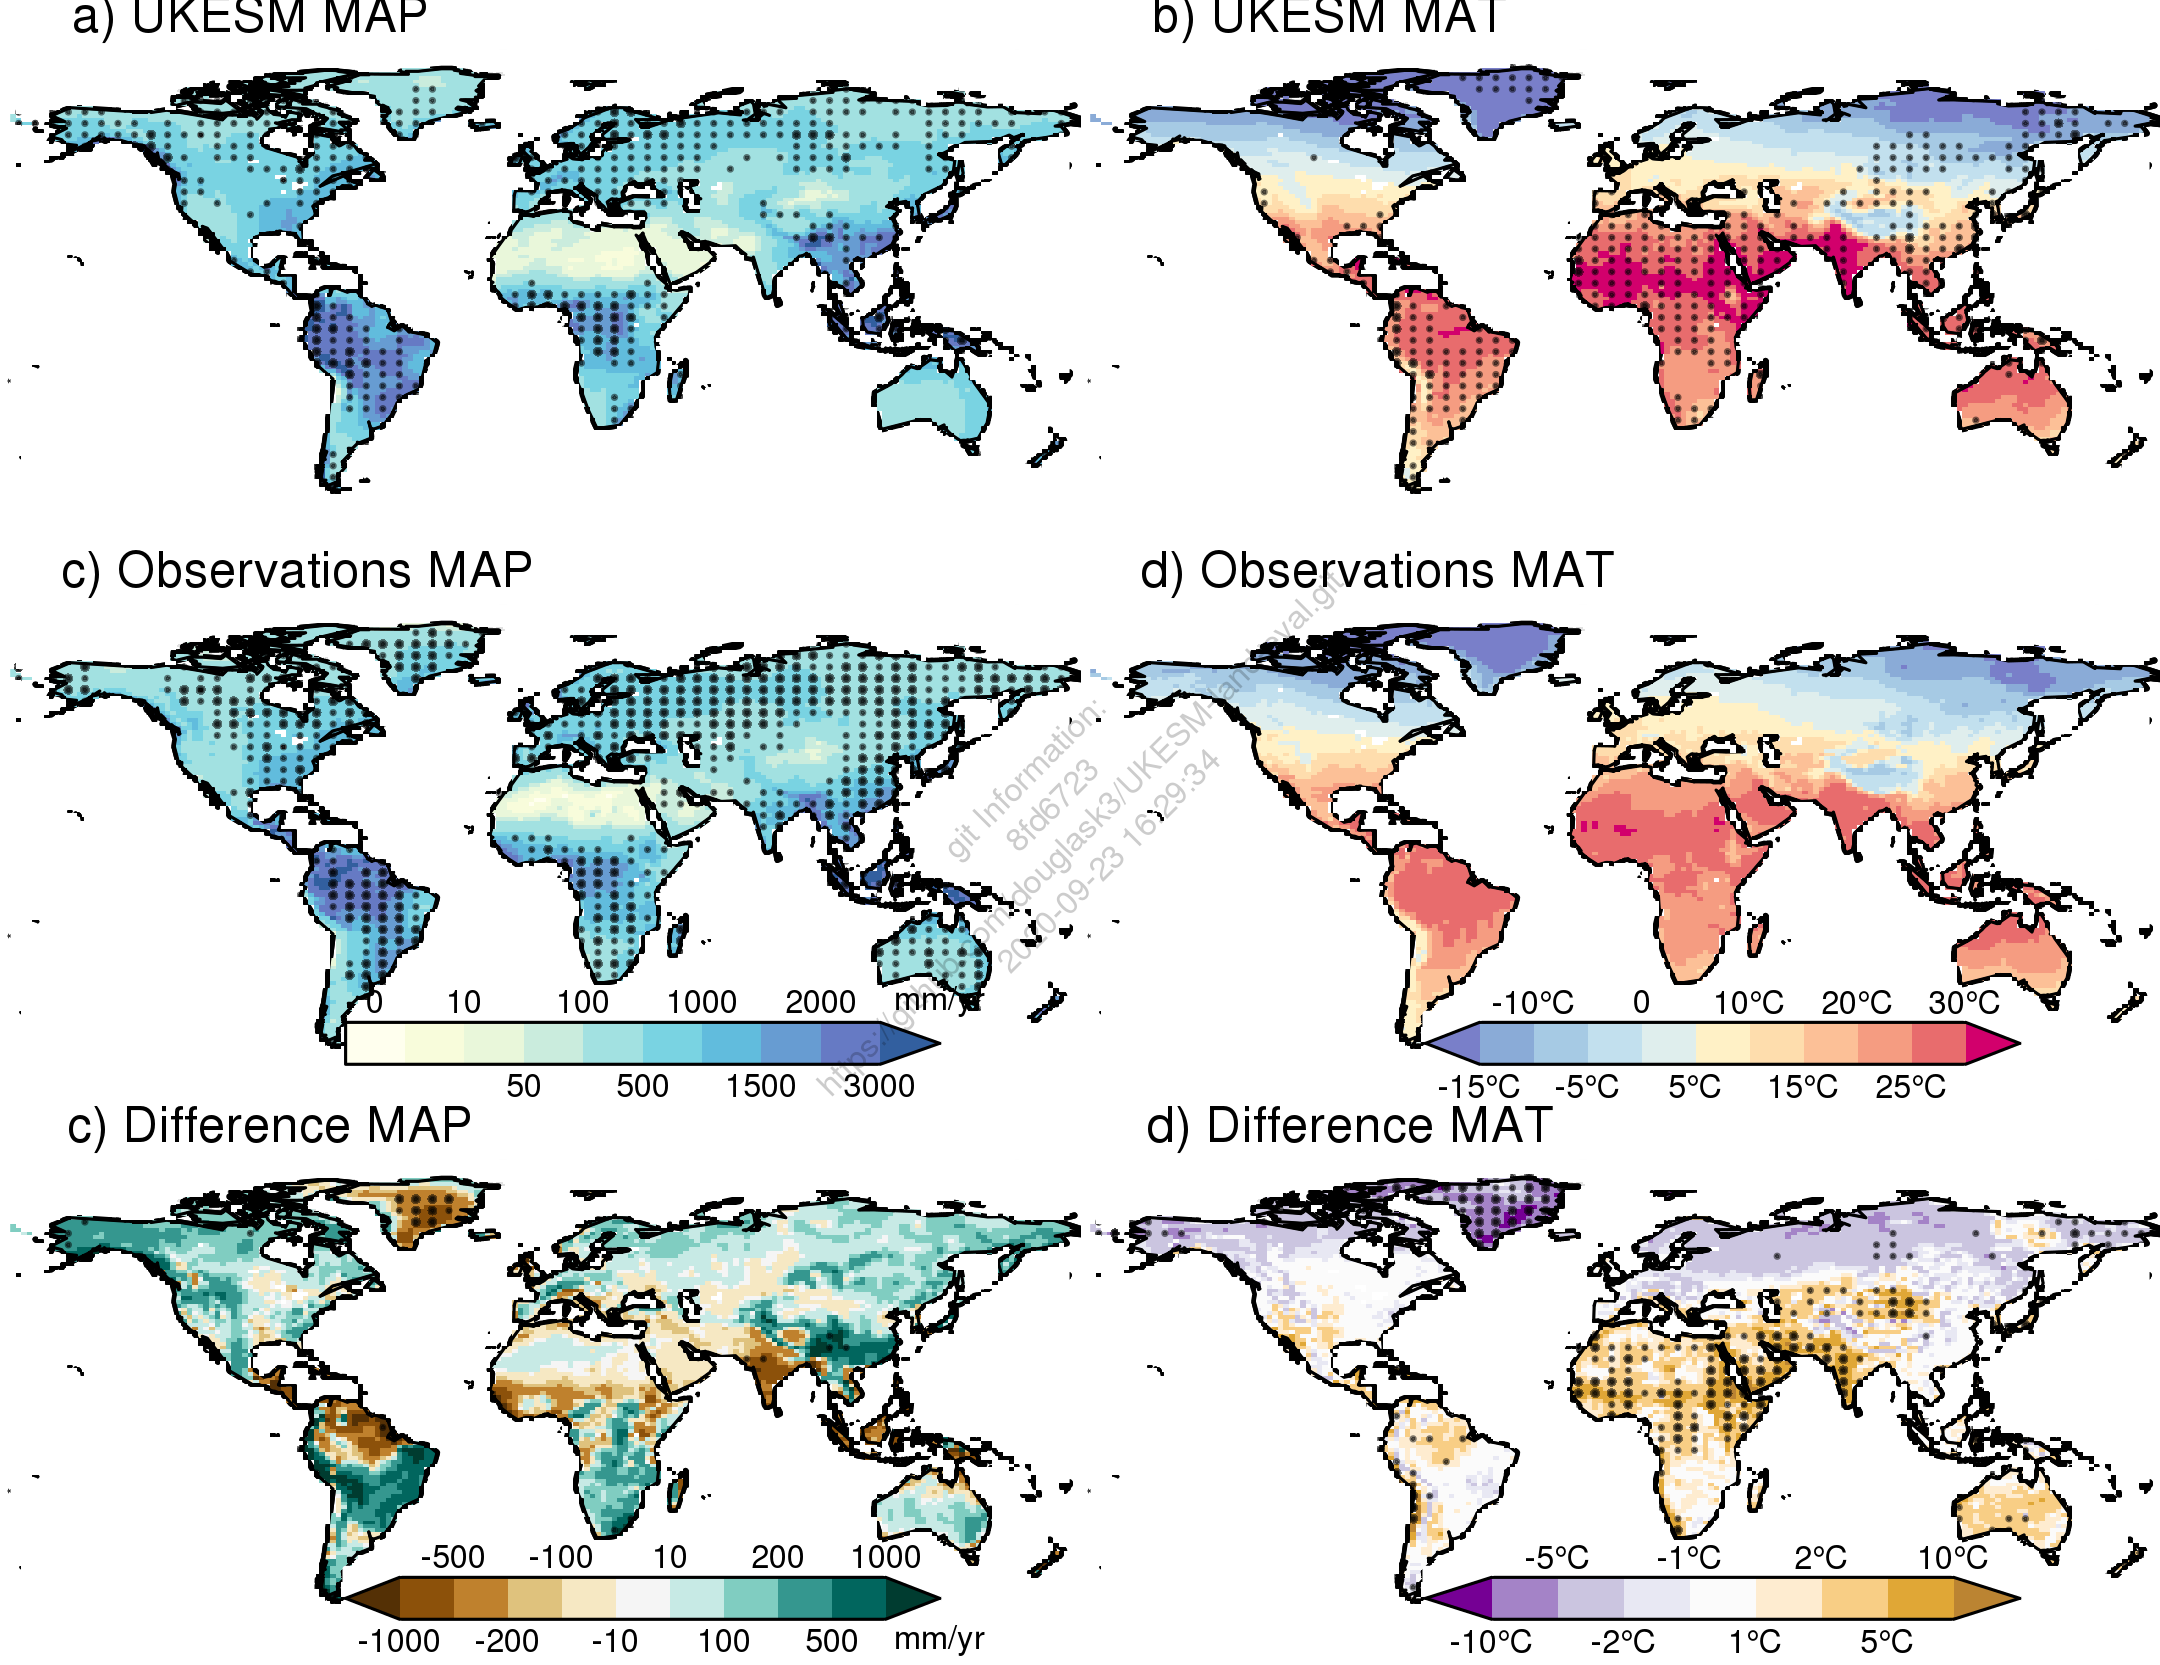
\includegraphics[width=12cm]{figs/Climate/annual_average_clims.png}
    \caption{Climate comparison \label{fig:ClimateAAMaps}}
\end{figure*}

%\subsection{Soil moisture}
%\hilight{Ranjini?} 
%this is in here for HadGEM3 - %https://agupubs.onlinelibrary.wiley.com/doi/full/10.1029/2018MS001370

\subsubsection{Cold processes including albedo}
\hilight{Eleanor - we need to decide what is different between JULEs-ES and GL7 - I suspect we actually need only an albedo plot}
\hilight{Eleanor - bit of text & can I get original figures (they didnt copy into google docs vert well)}
\hilight{Rob P - want to make a plot?}

\subsubsection{LST}
\hilight{Rob K}

\subsubsection{Drought}
\hilight{Phil - bit of a summary of results}
\begin{figure*}[t]
    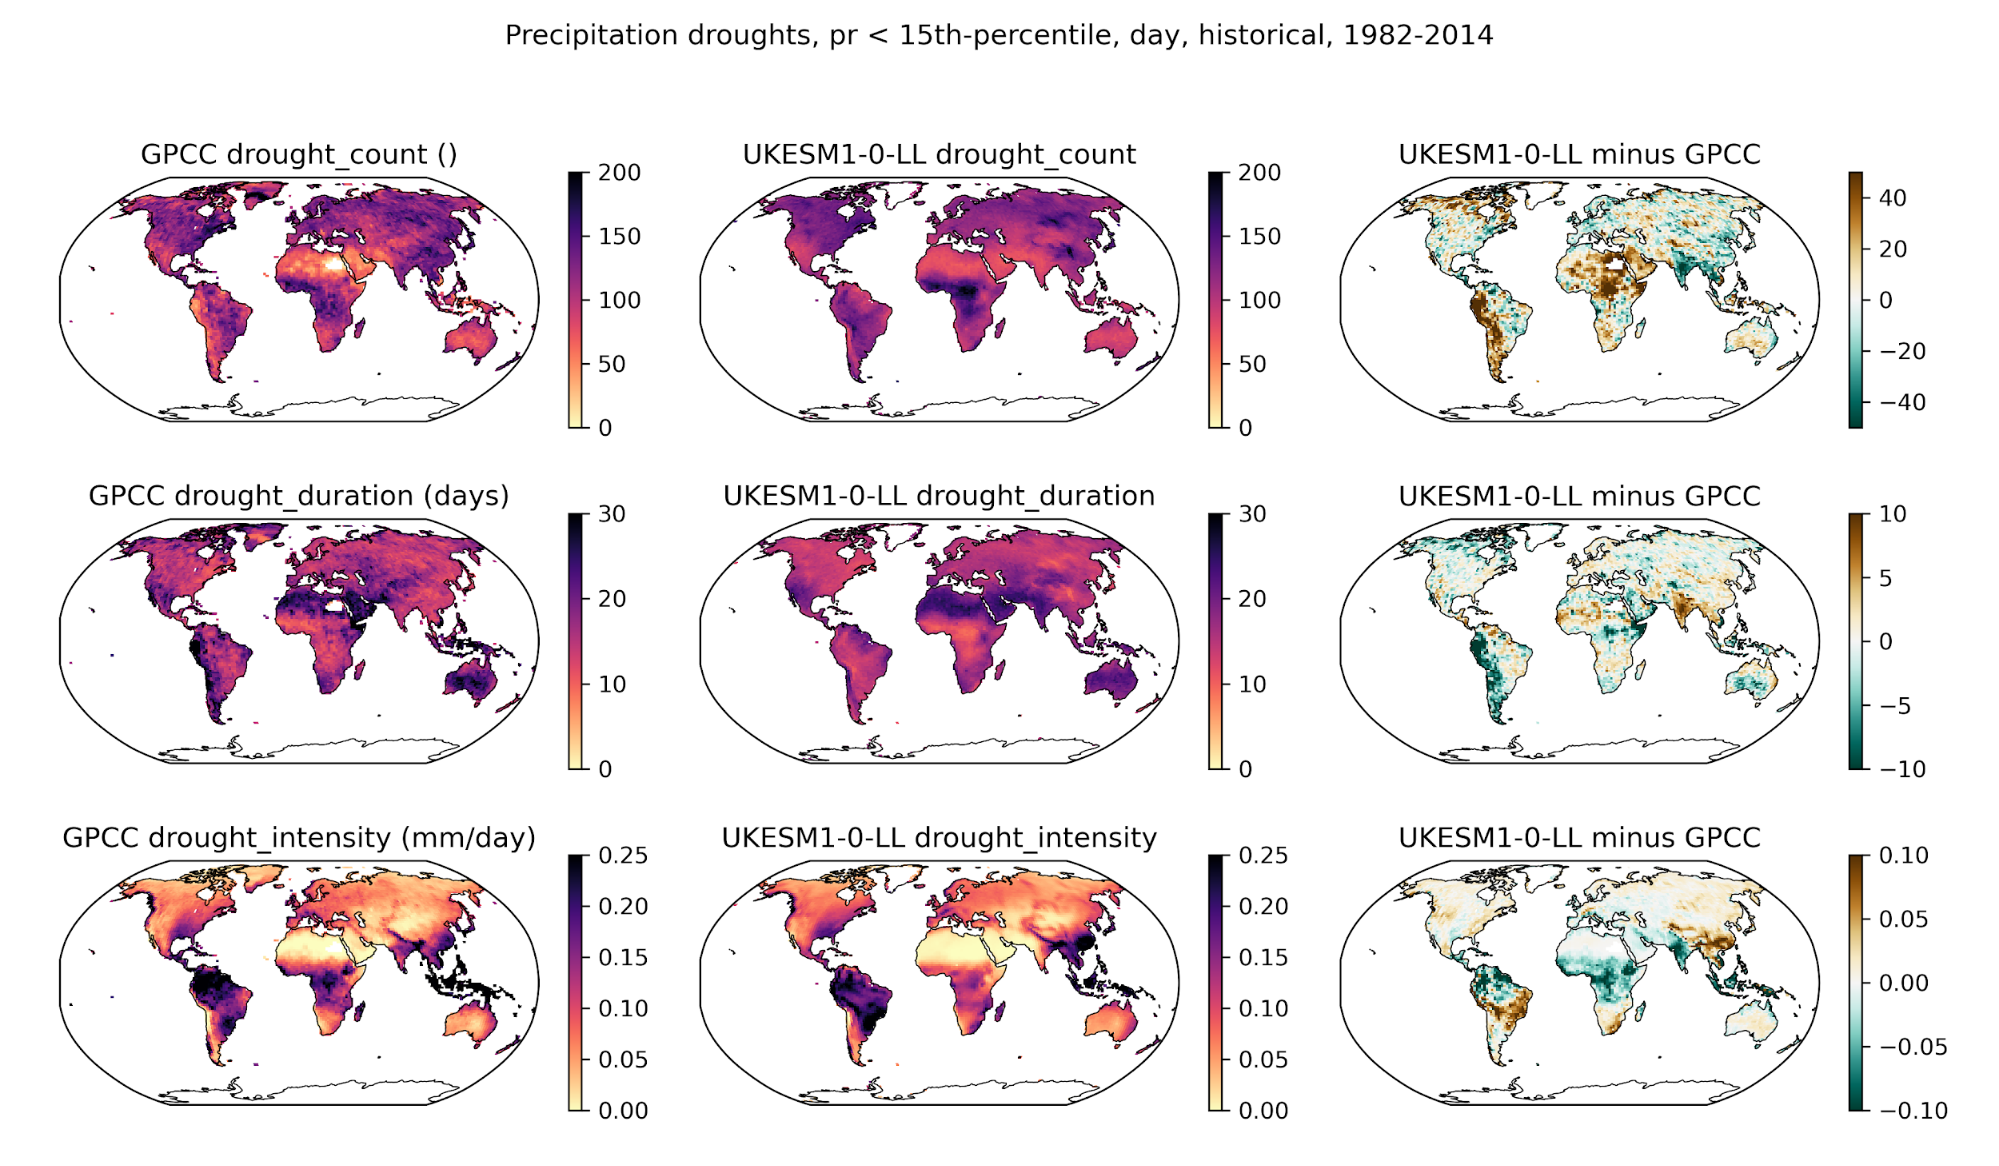
\includegraphics[width=6cm]{figs/drought.png}
    \caption{Caption Phil? \label{fig:drought} }
\end{figure*}



\subsection{Vegetation Distribution}
\begin{itemize}
    \item A lack on mix of tree and herb cover in much of the world, particularly Australia, Africa, Temperate America. The same could be true for Boreal regions, though there is disagreement in the observations here.
    \item Australia and SE Asia also show to tight a transition from non-vegetated to vegetated (R2 in Fig. \ref{fig:VegDistTri})
    \item causes too much tree cover extent and, in some places, to much bare ground with very rapid transitions (Figure  \ref{fig:VegDistMap}).
    \item grass extent is generally to small, but where grass does occur, there is too much of it.
    \item Too much bare soil in SE Asia, North Africa, possibly in Australia though depending on observations
    \item Too extensive in South Africa, North Africa, Boreal America, SE Asia, 
\end{itemize}


\begin{figure*}[t]
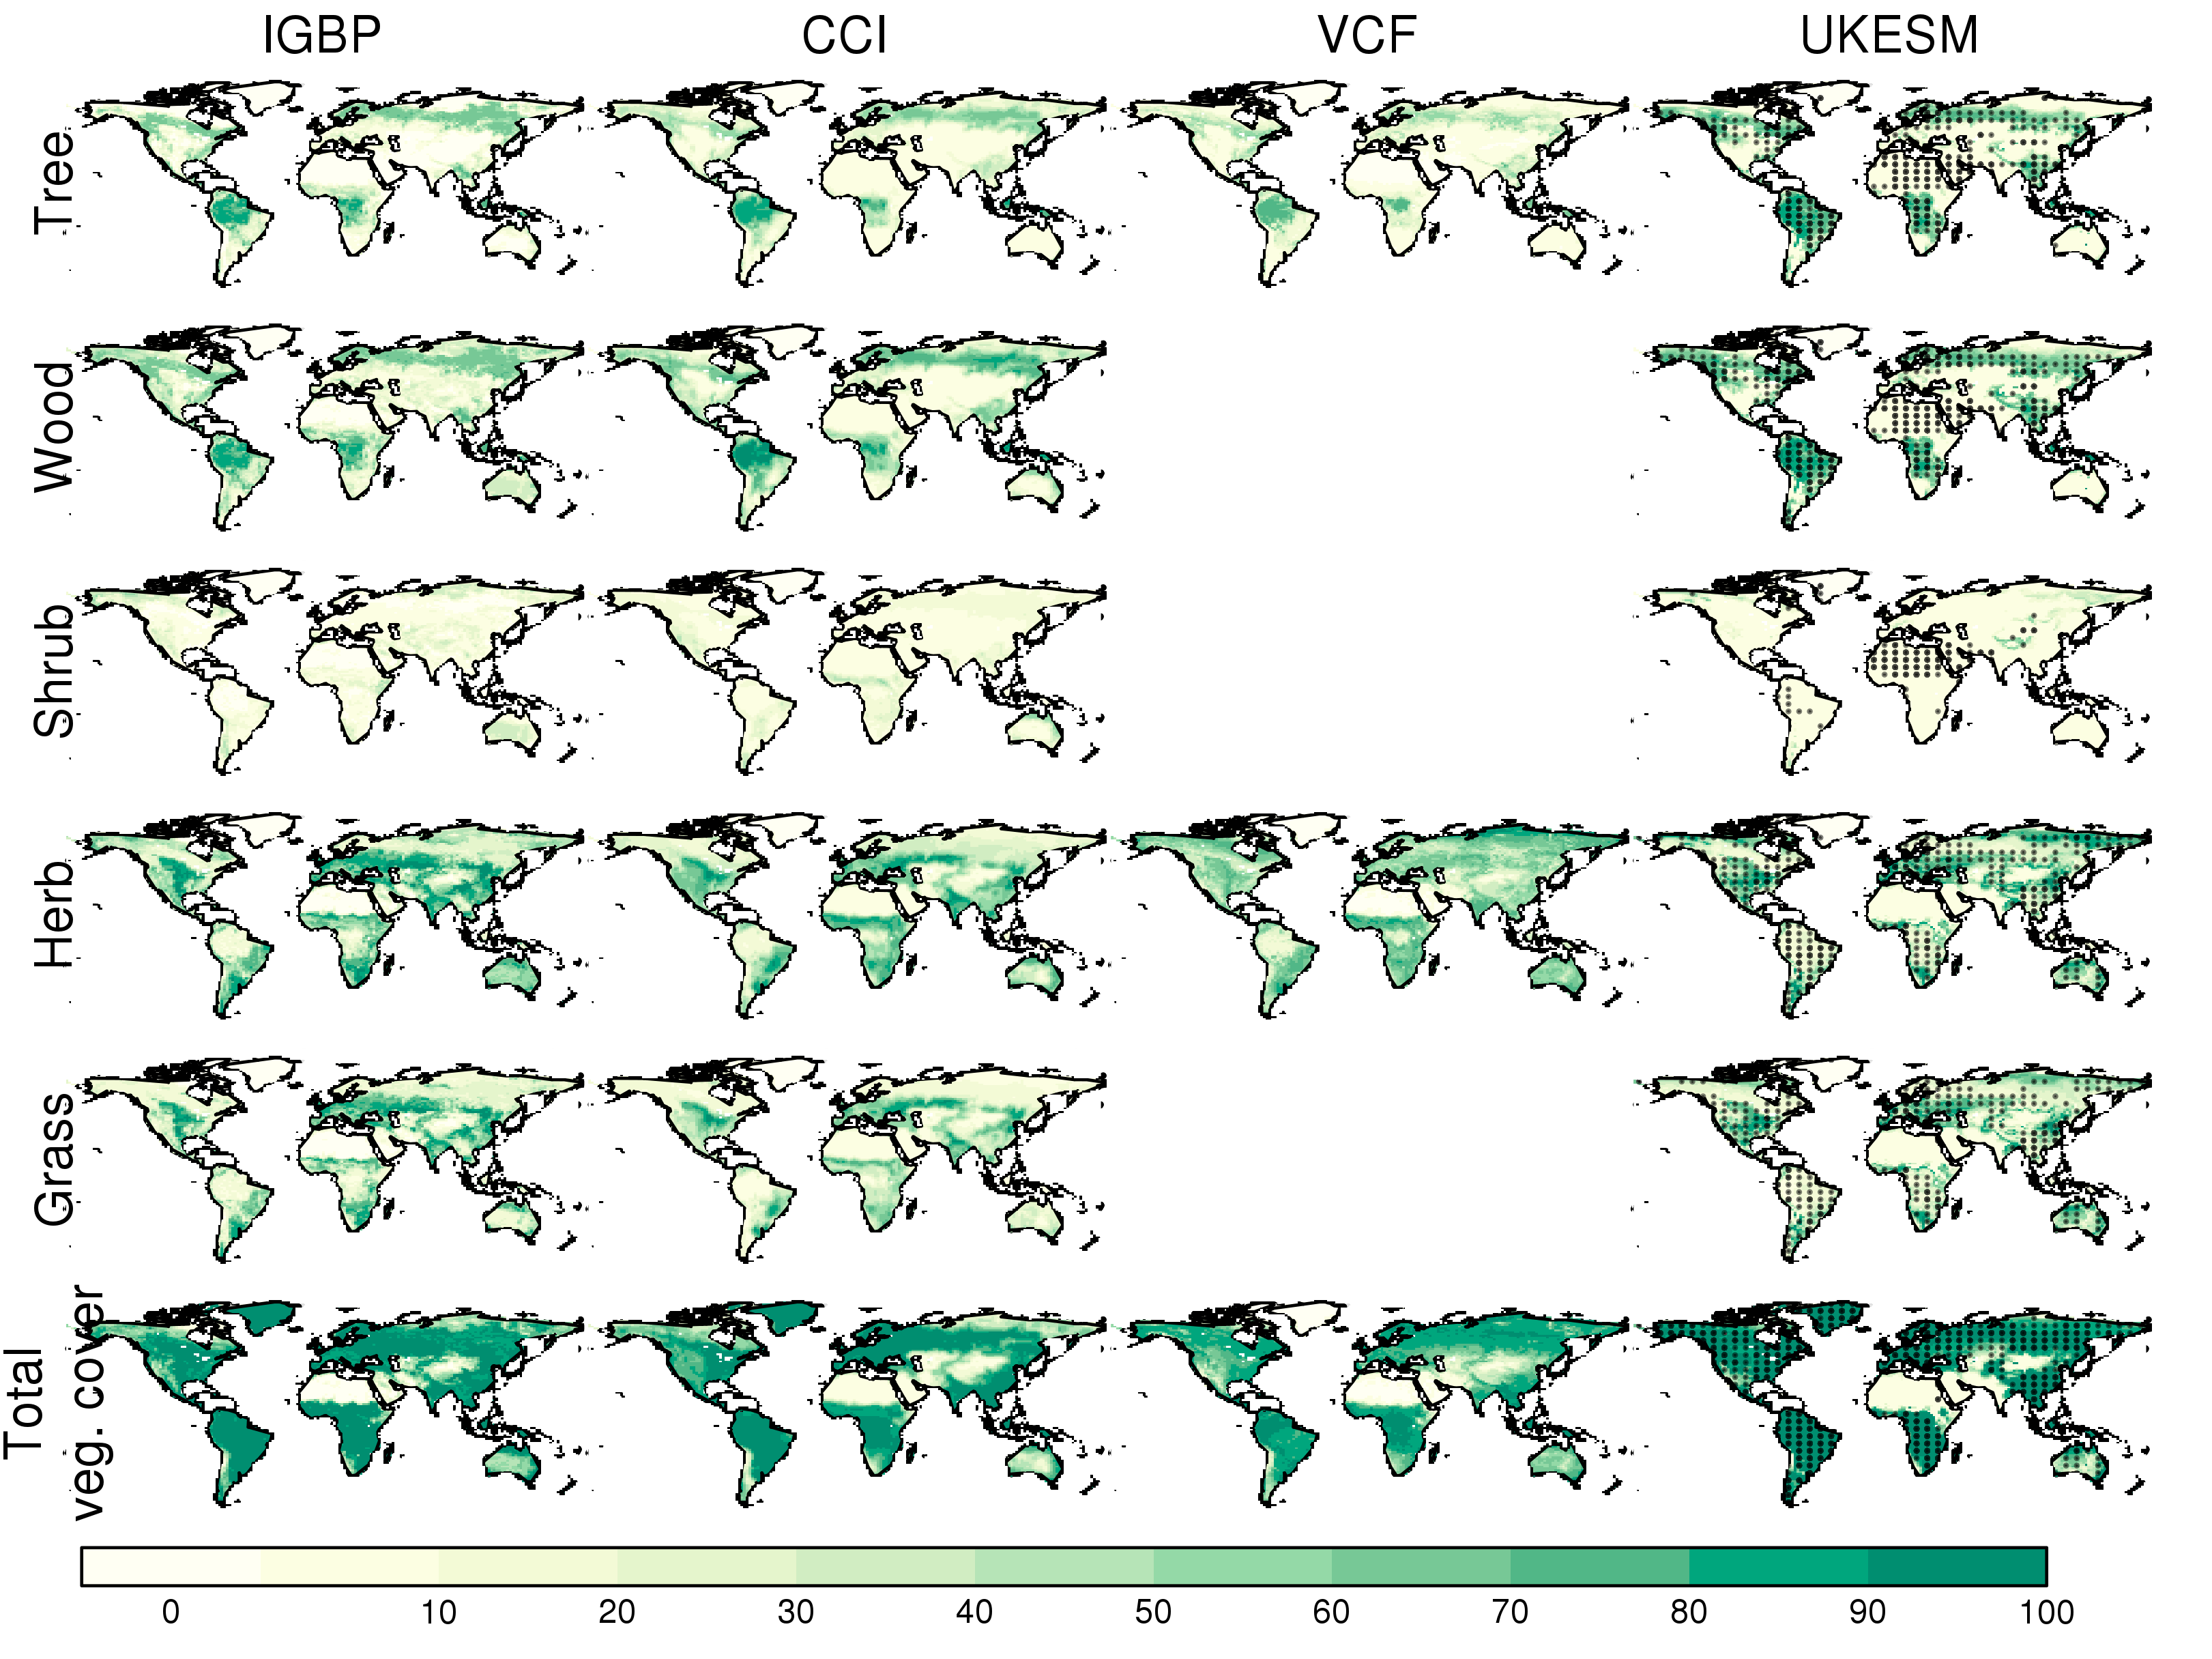
\includegraphics[width=12cm]{figs/VegDist/vegDist.png}
\caption{Observed vs simulated percentage vegetation cover. From top to bottom: Tree, wood, shrub, herb, grass and total vegetative cover. From left to right, IGBP <<ref>>, CCI <<ref>>, VCF <<ref>> observations and simulated by UKESM. Dots in the UKESM column show variation in ensemble members \label{fig:VegDistMap}}
\end{figure*}

\begin{figure}[t]
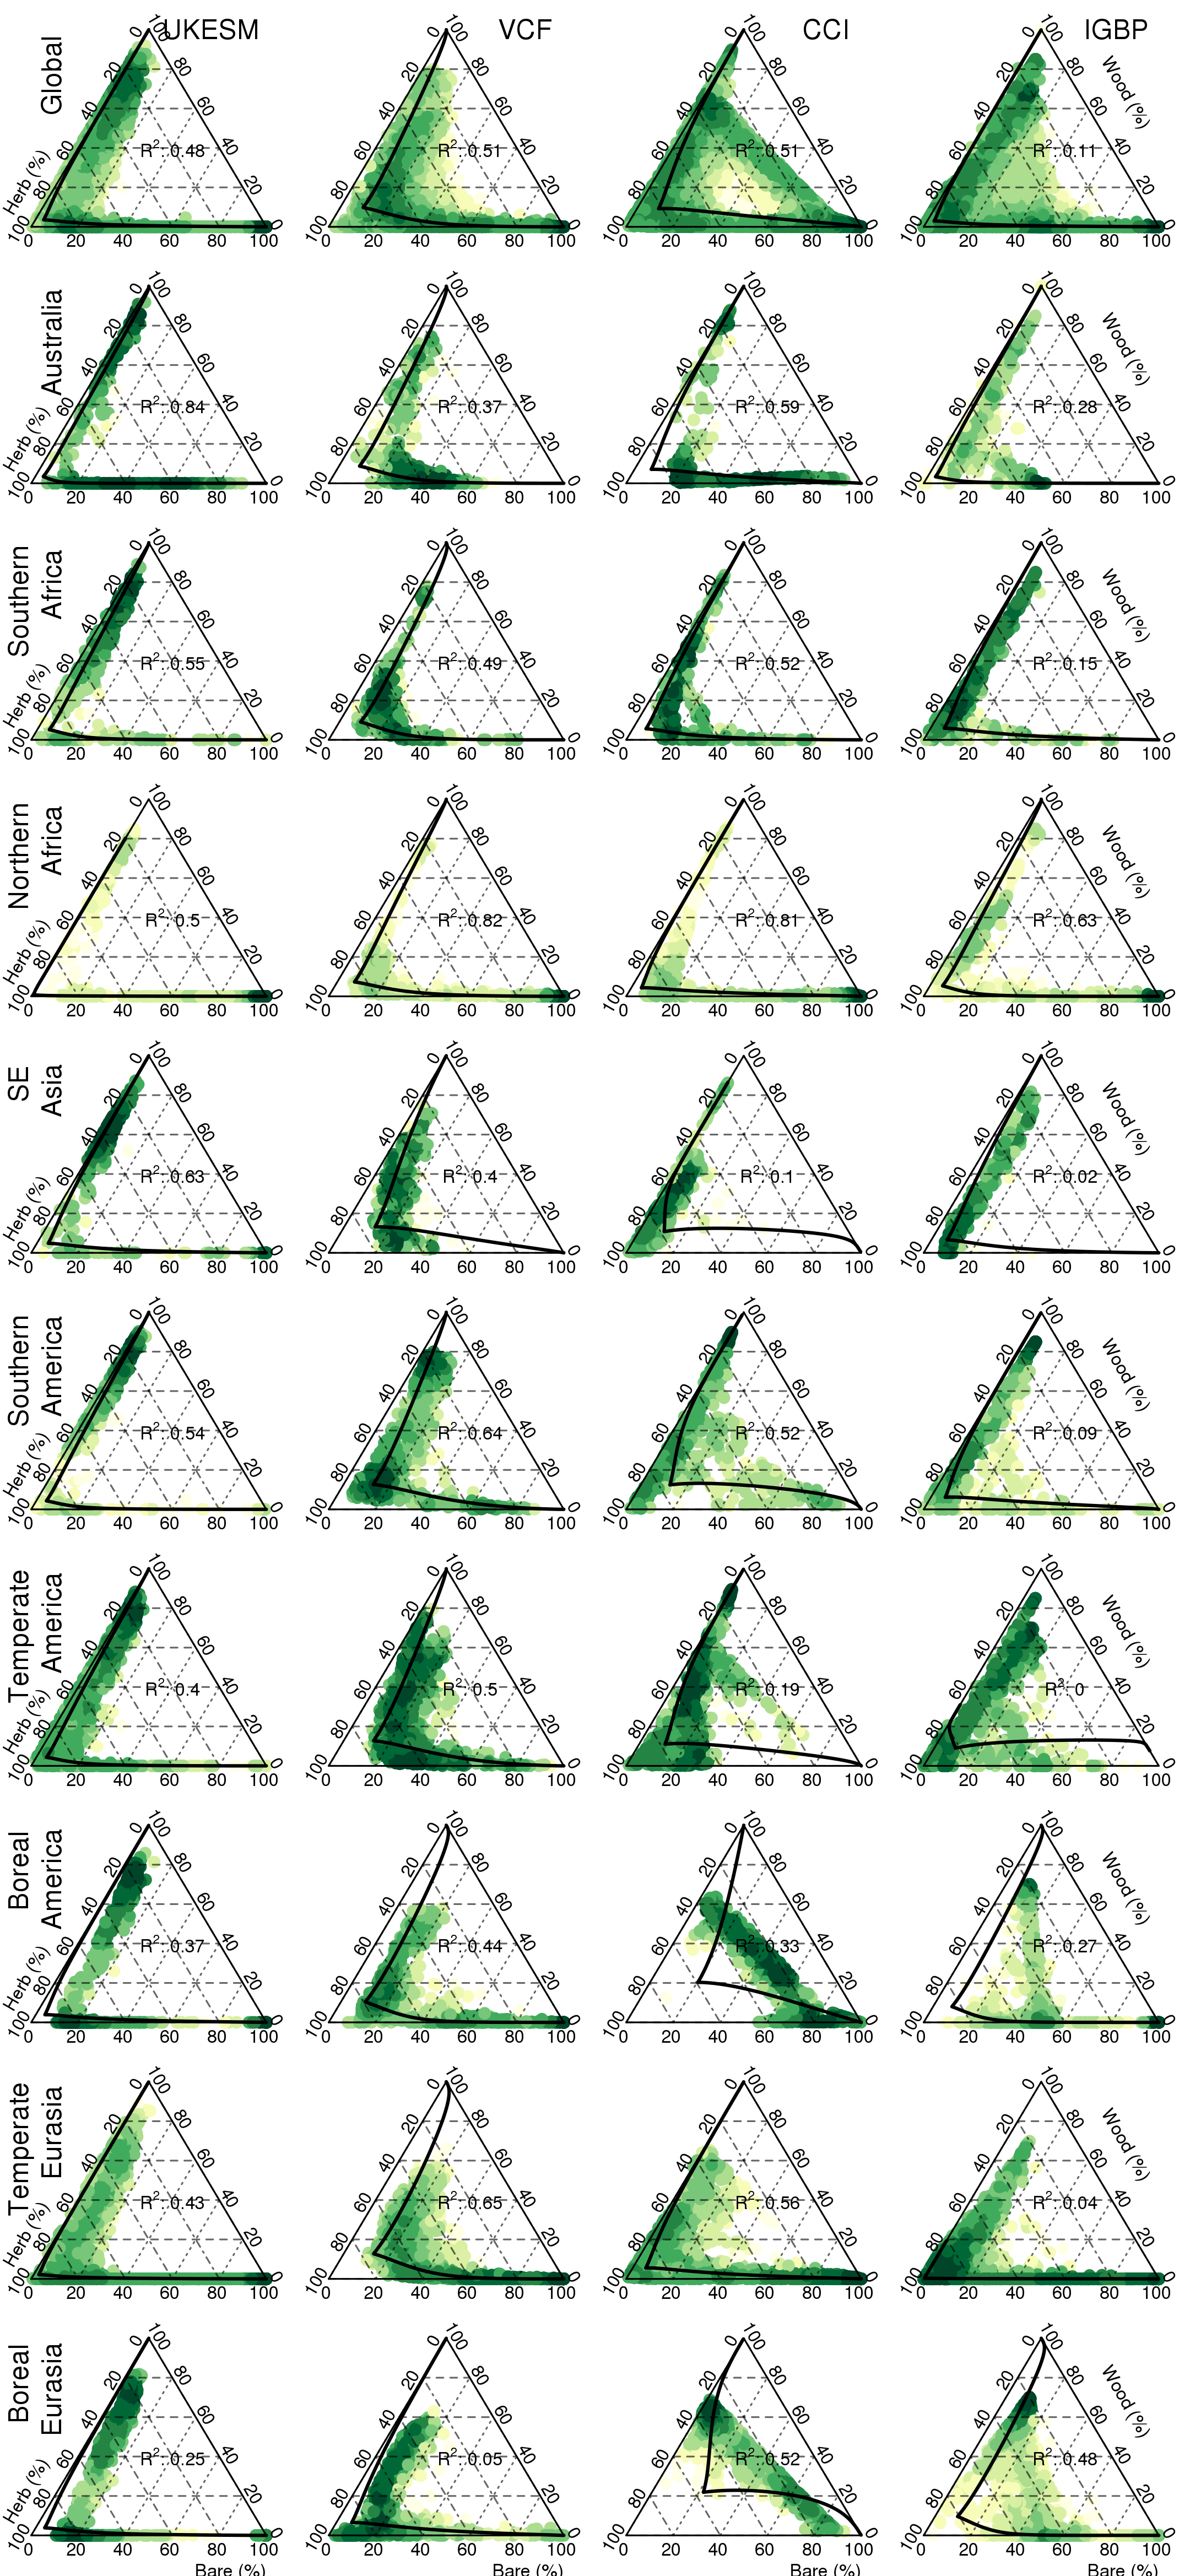
\includegraphics[width=8.3cm]{figs/VegDist/VegDistTriangle.png}
\caption{Tree (right axis), grass (left axis) and bare cover (bottom axis) variations over possible vegetated land (i.e excluding urban and water). Top row show global distributions and subsequent rows for each realm (Fig. \ref{fig:regionsMap}). First column as simulated by UKESM enemble mean, and subsequent columns for VCF, CCI, IGBP obervations <<add refs>> \label{fig:VegDistTri}}
\end{figure}


\hilight{Rebecca - I would if we could also do a veg fraction "turnover"?}

\subsection{Phenology}

\hilight{Doug - update with new LAI product}

\begin{figure*}[t]
    %\begin{subfigure}
        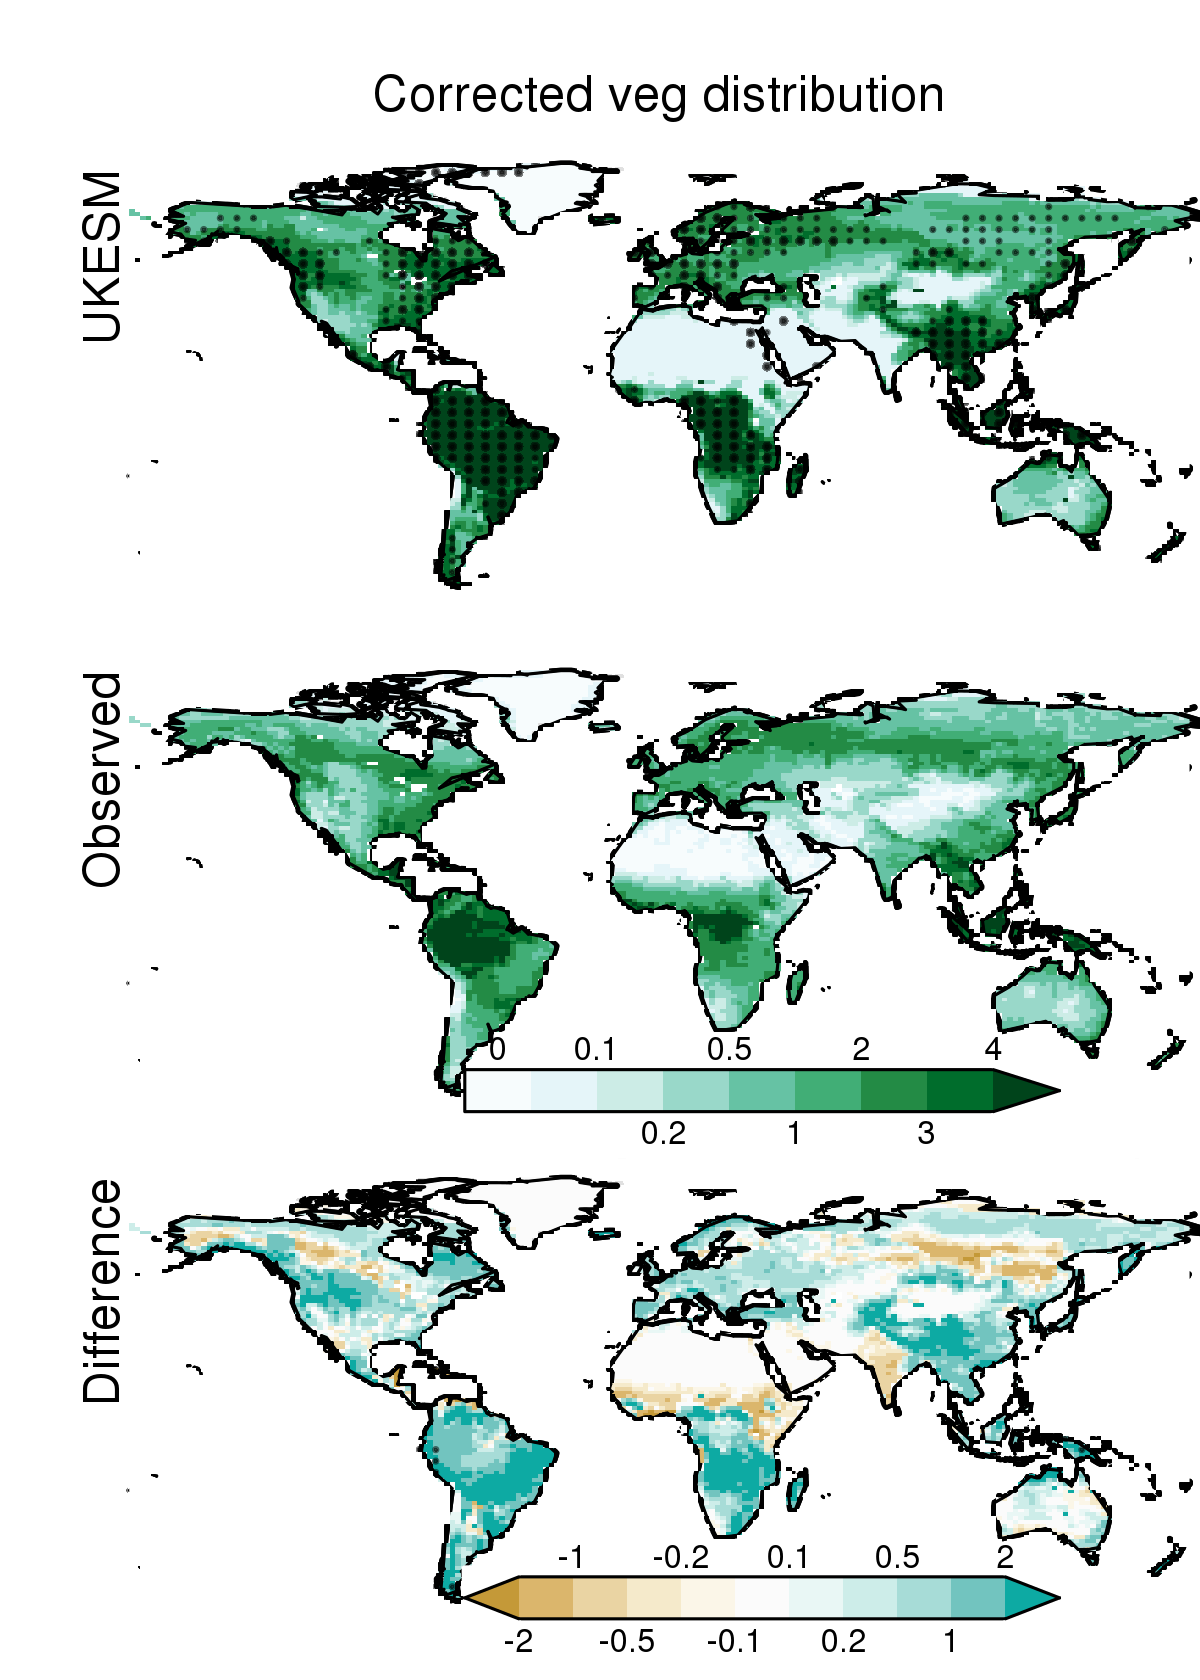
\includegraphics[width=5cm]{figs/LAI/fire_var_seasonality-maps-AA-mapscontrol-lai.png}
    %\end{subfigure}
    %\begin{subfigure}
        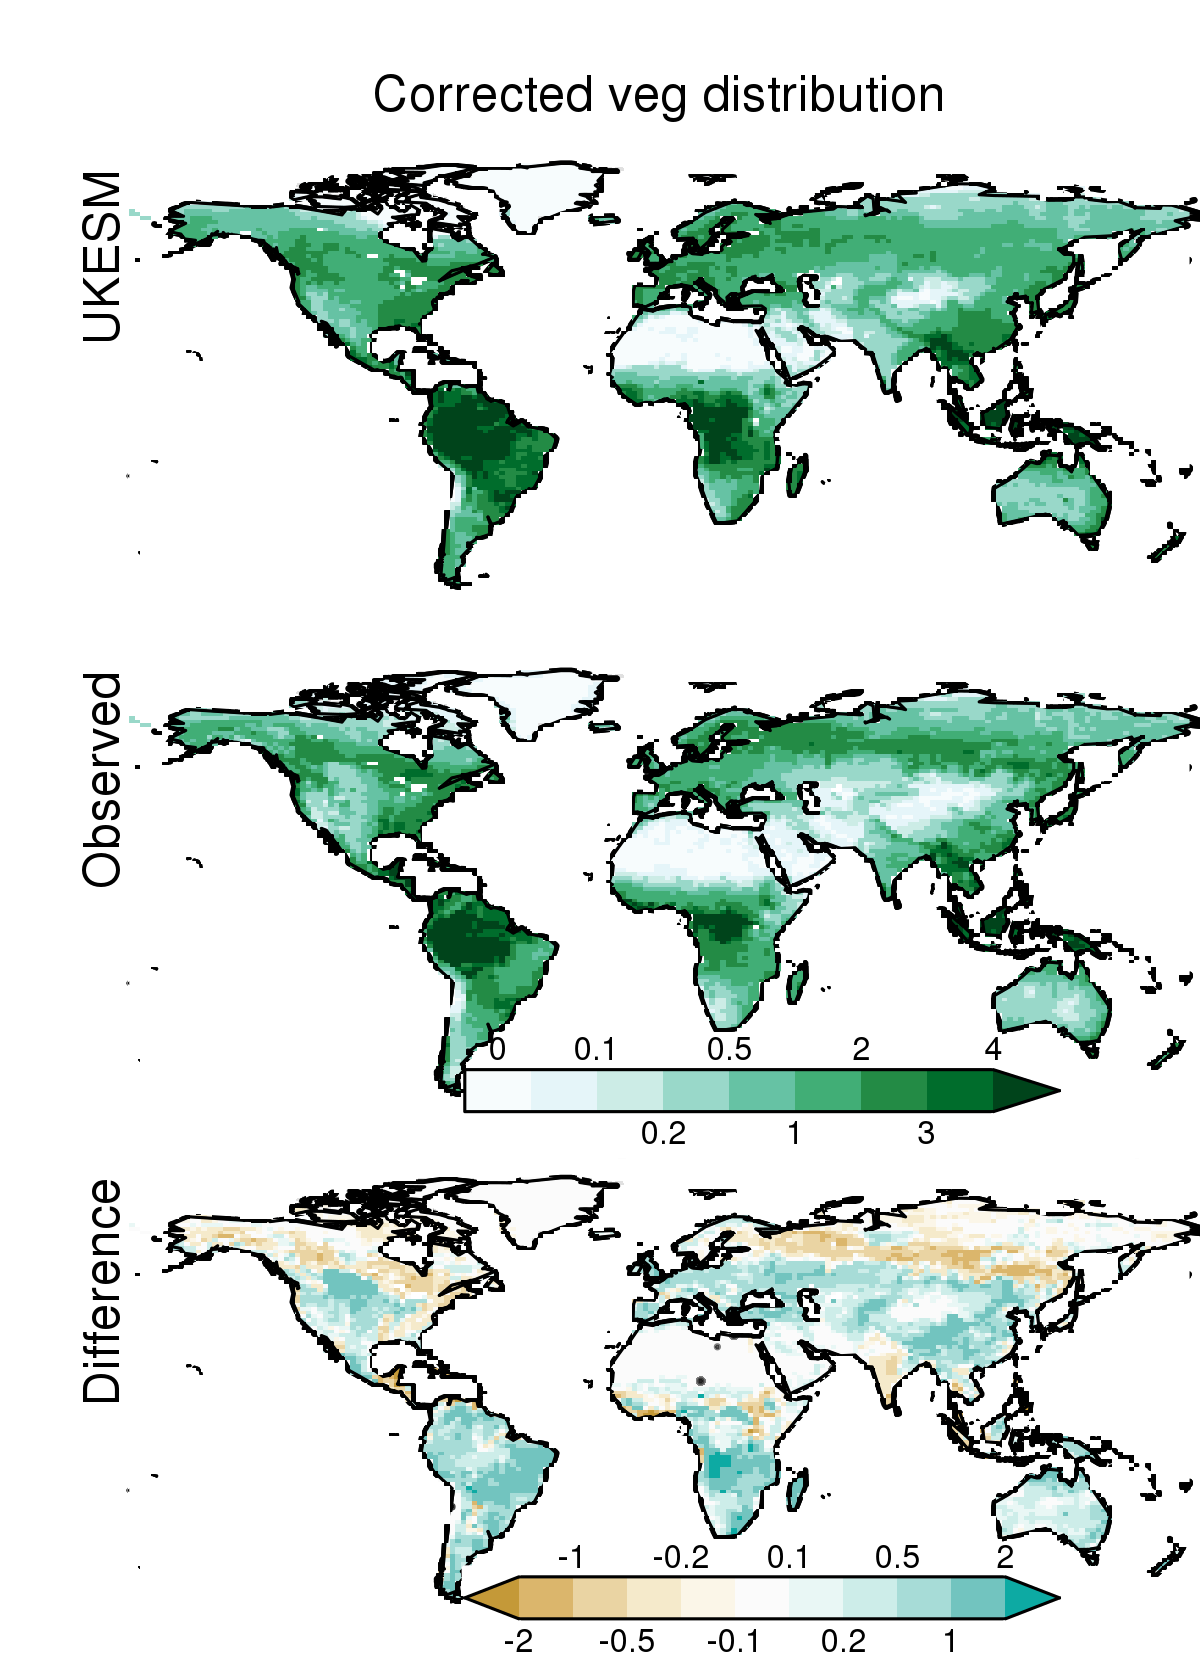
\includegraphics[width=5cm]{figs/LAI/fire_var_seasonality-maps-AA-mapsobsVegDist-lai.png}
    
    %\end{subfigure}
    \caption{Simulated (top), observed (middle, <<ref>>) and different in mean annual LAI for 2001-2013. Right hand, UKESM has been corrected for vegetation distribution biases \label{fig:LAImap}}
\end{figure*}

\begin{figure*}[t]
    %\begin{subfigure}
        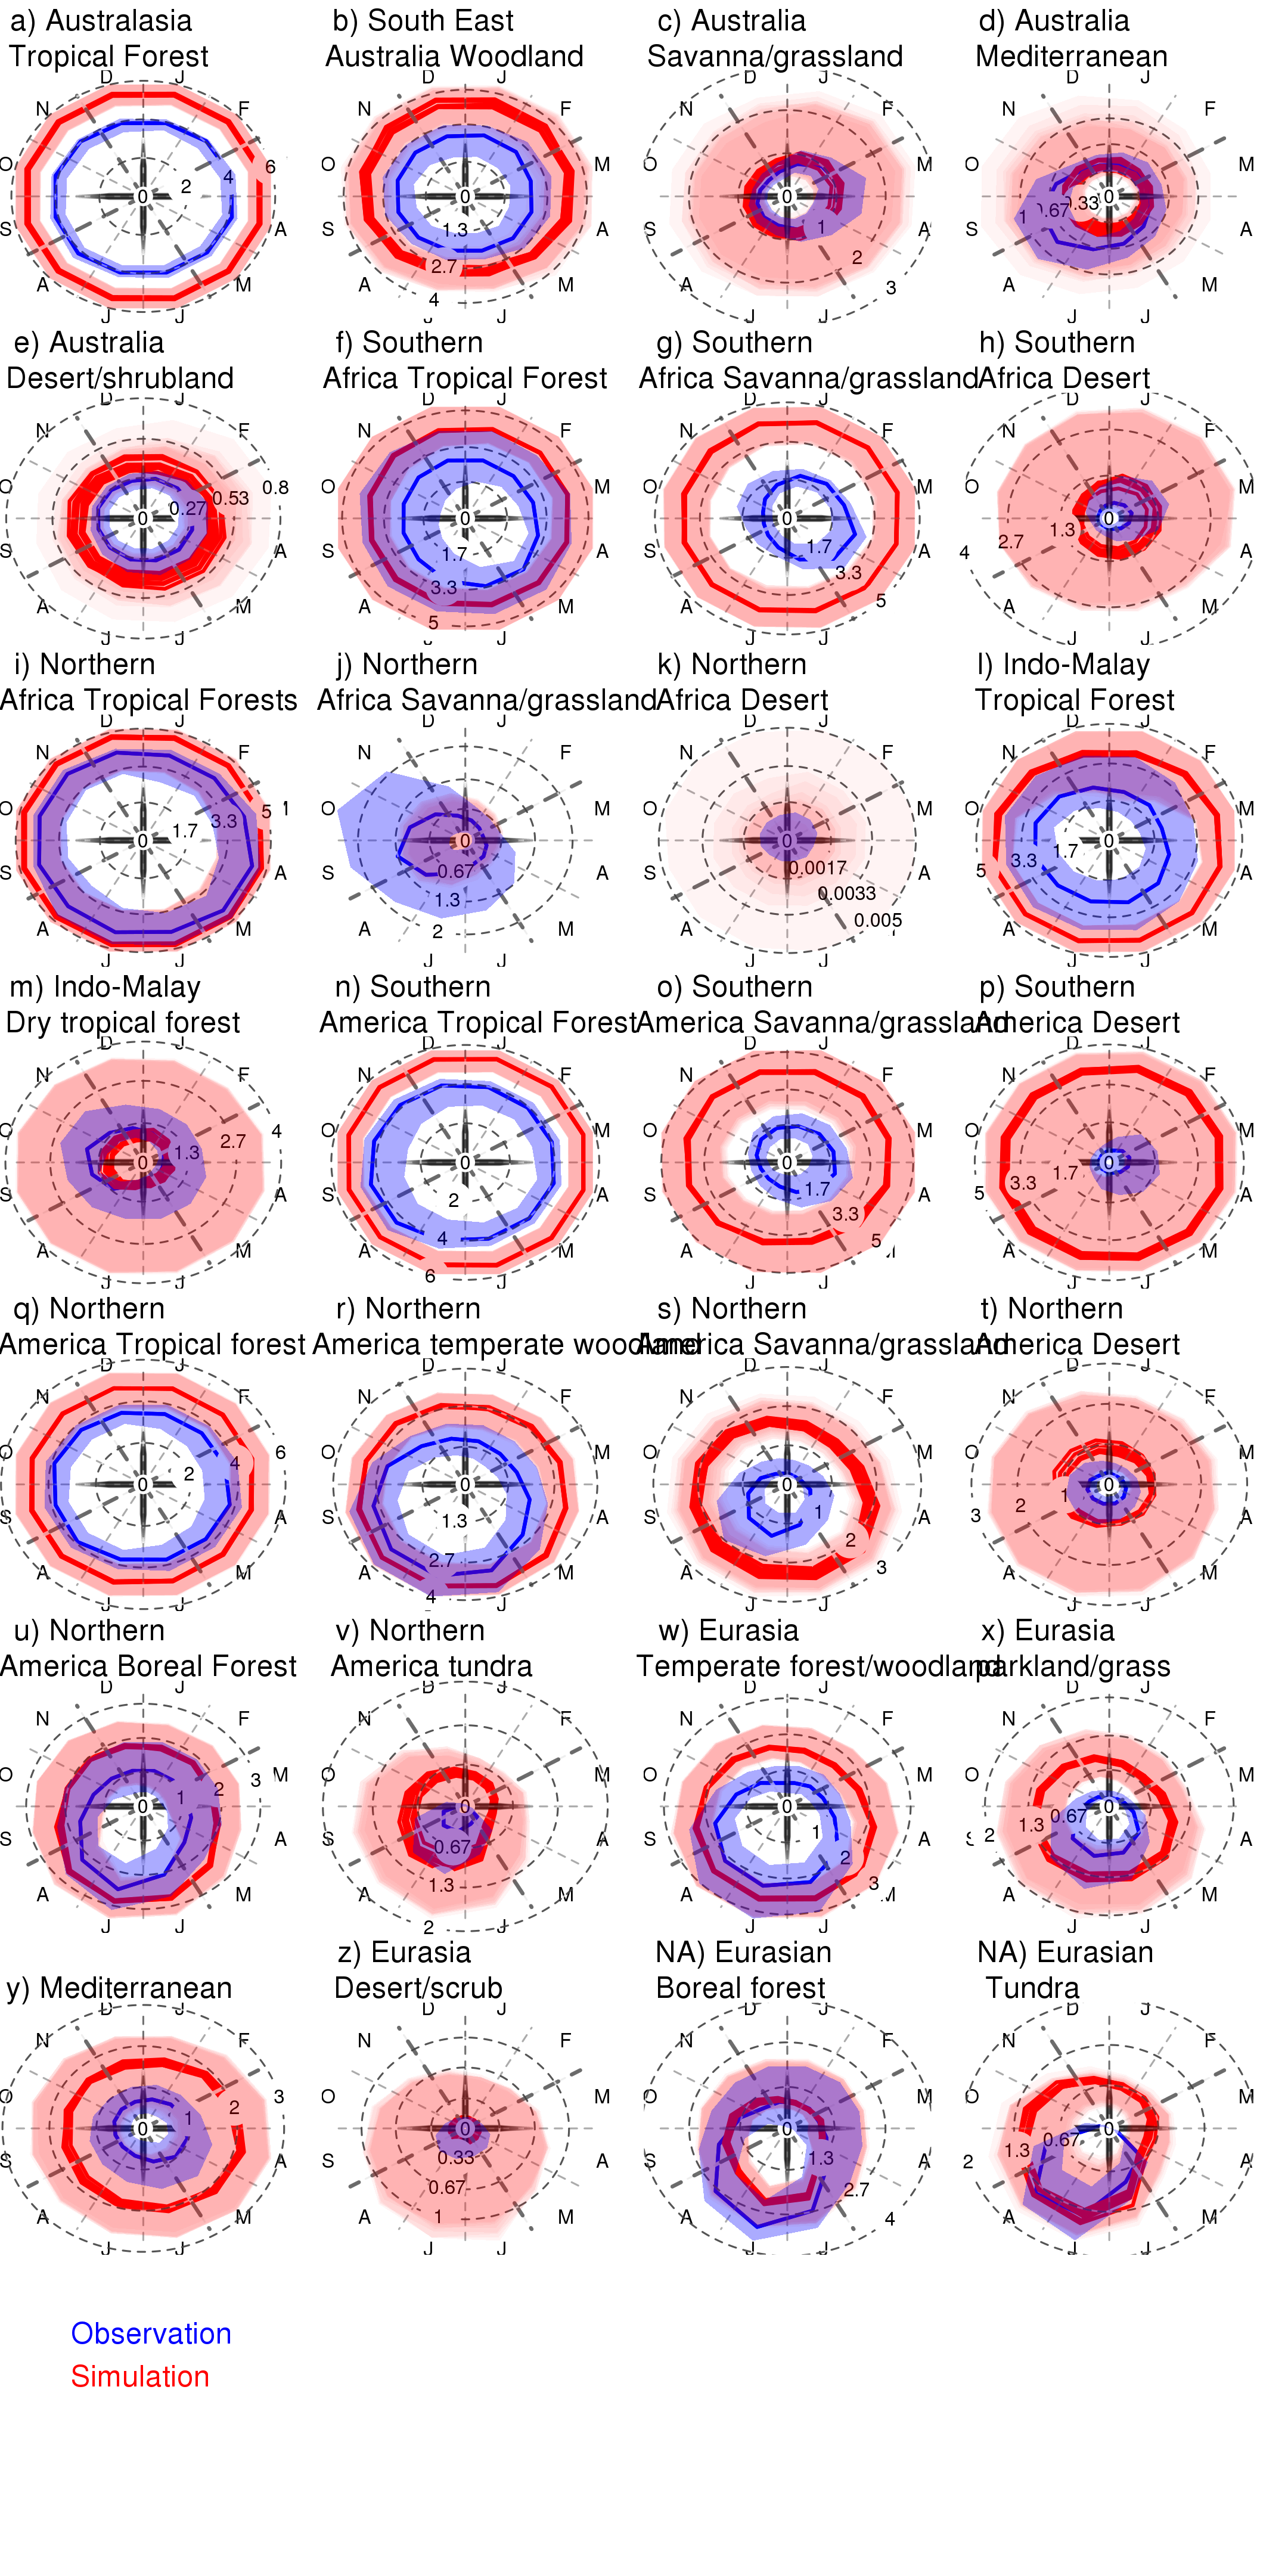
\includegraphics[width=5cm]{figs/LAI/fire_var_seasonality-TS-control-lai.png}
    %\end{subfigure}
    %\begin{subfigure}
        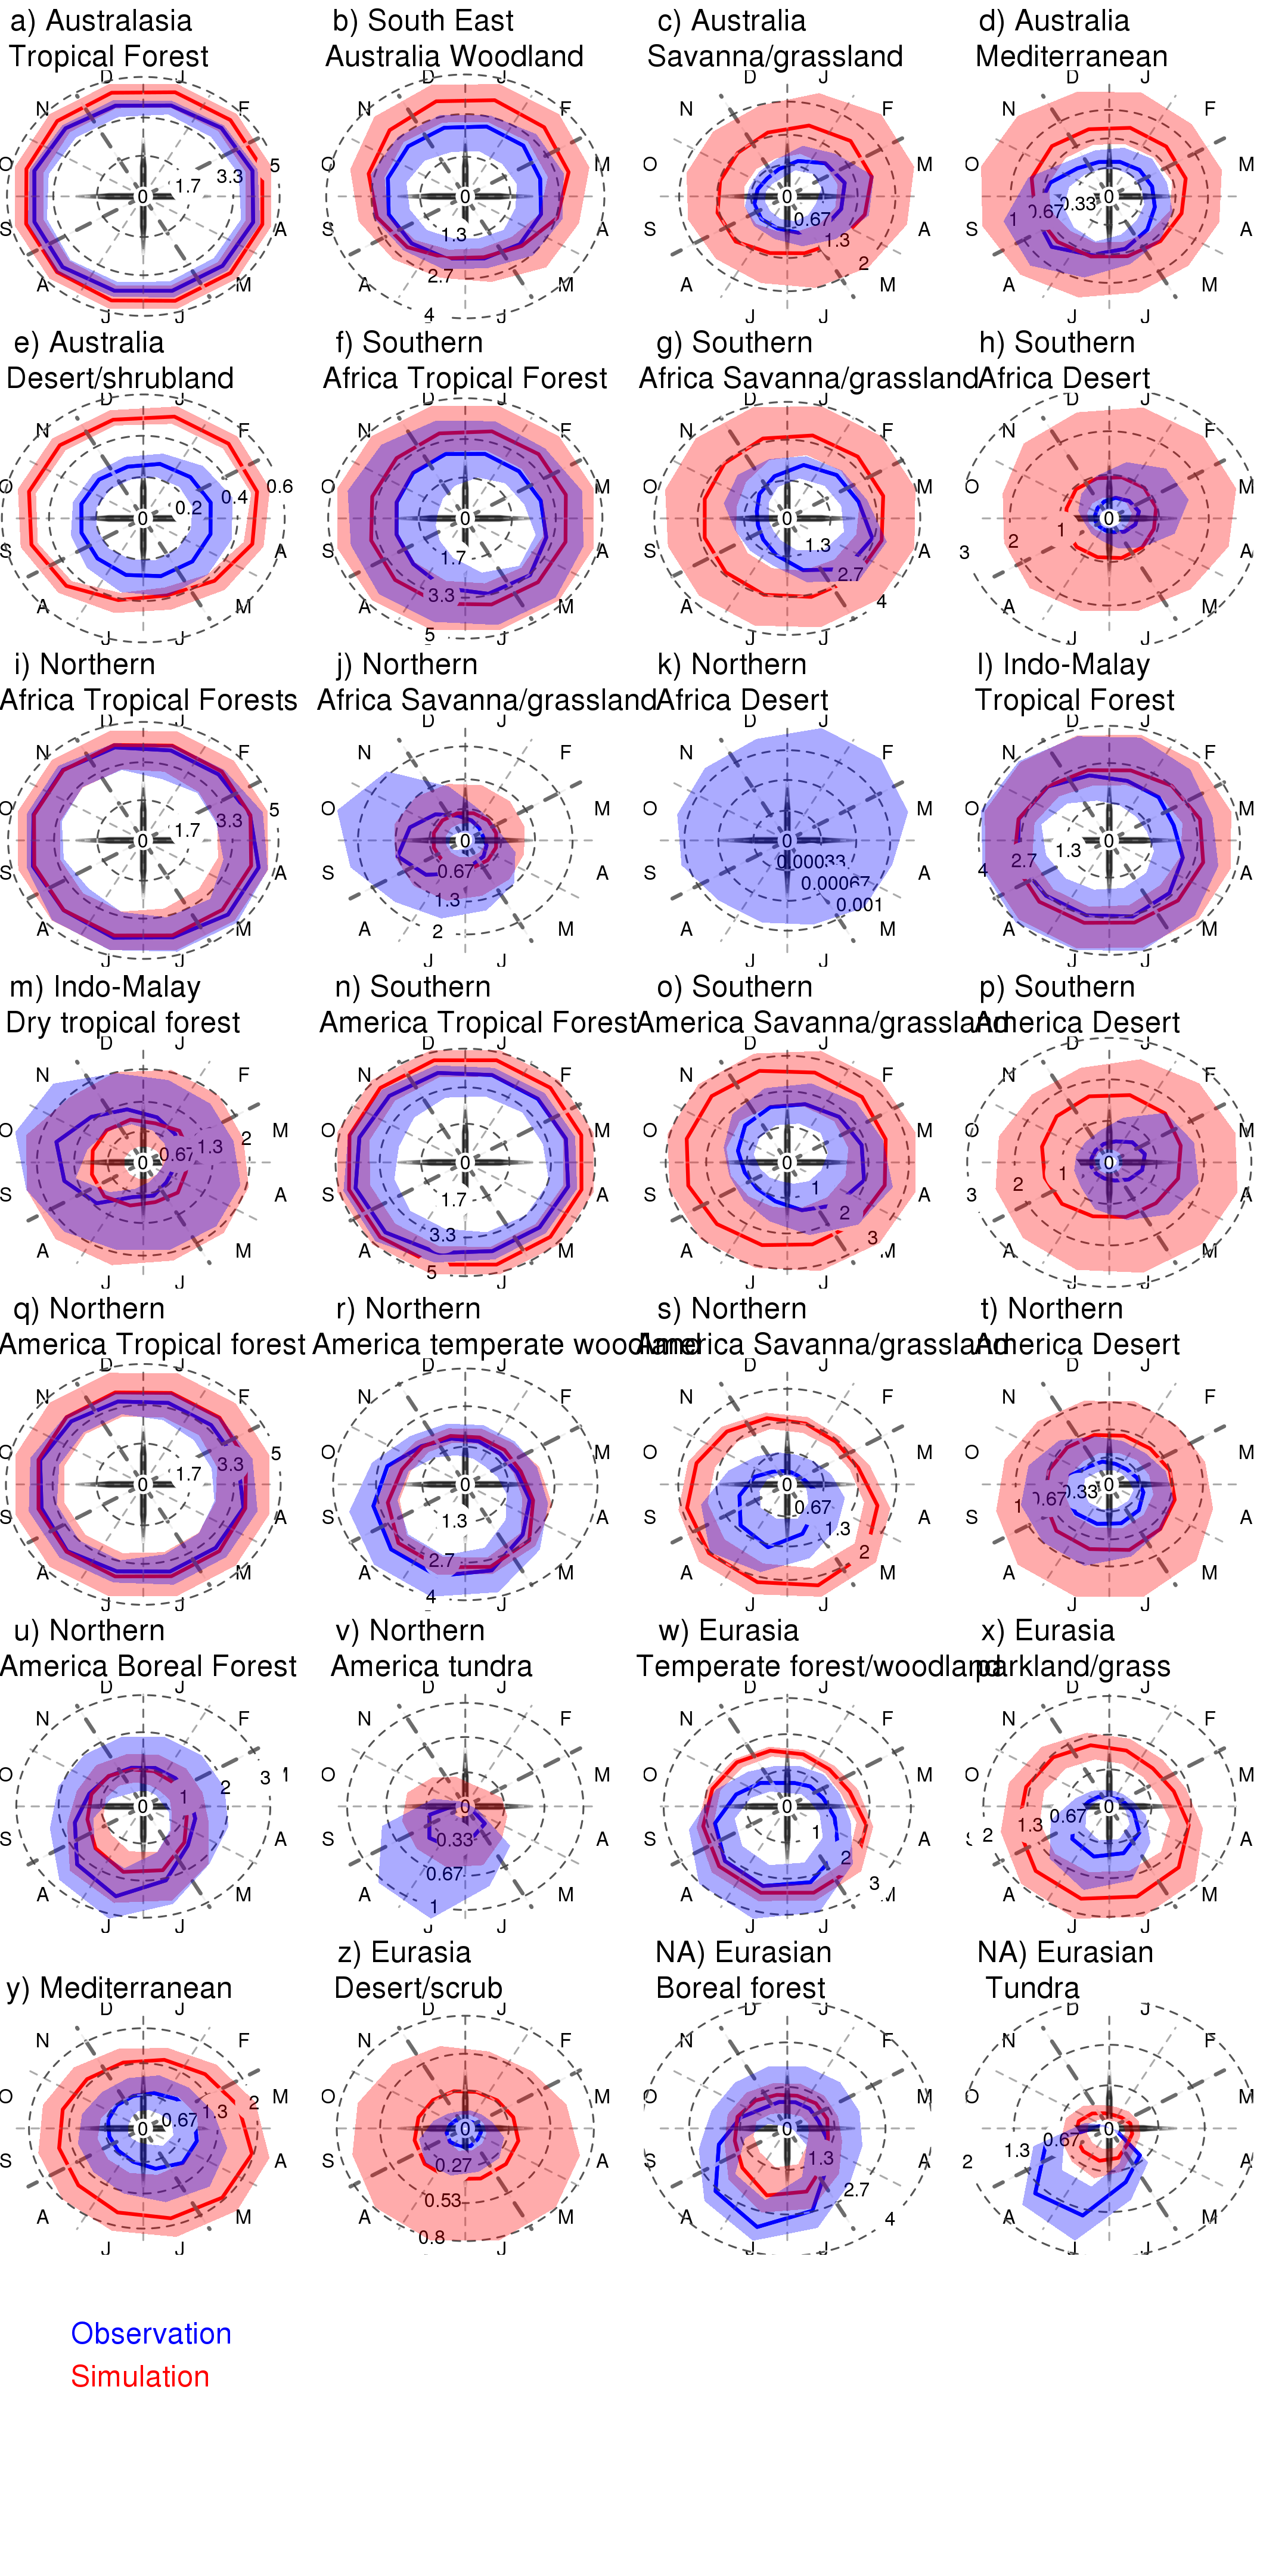
\includegraphics[width=5cm]{figs/LAI/fire_var_seasonality-TS-obsVegDist-lai.png}
    
    %\end{subfigure}
    \caption{Simulated (red), observed (blue, <<ref>>) and seasonal cycles in LAI for 2001-2013 for each region(see \ref{fig:regionsMap}. Right hand, UKESM has been corrected for vegetation distribution biases \label{fig:LAIseasonalTS}}
\end{figure*}

\begin{figure*}[t]
    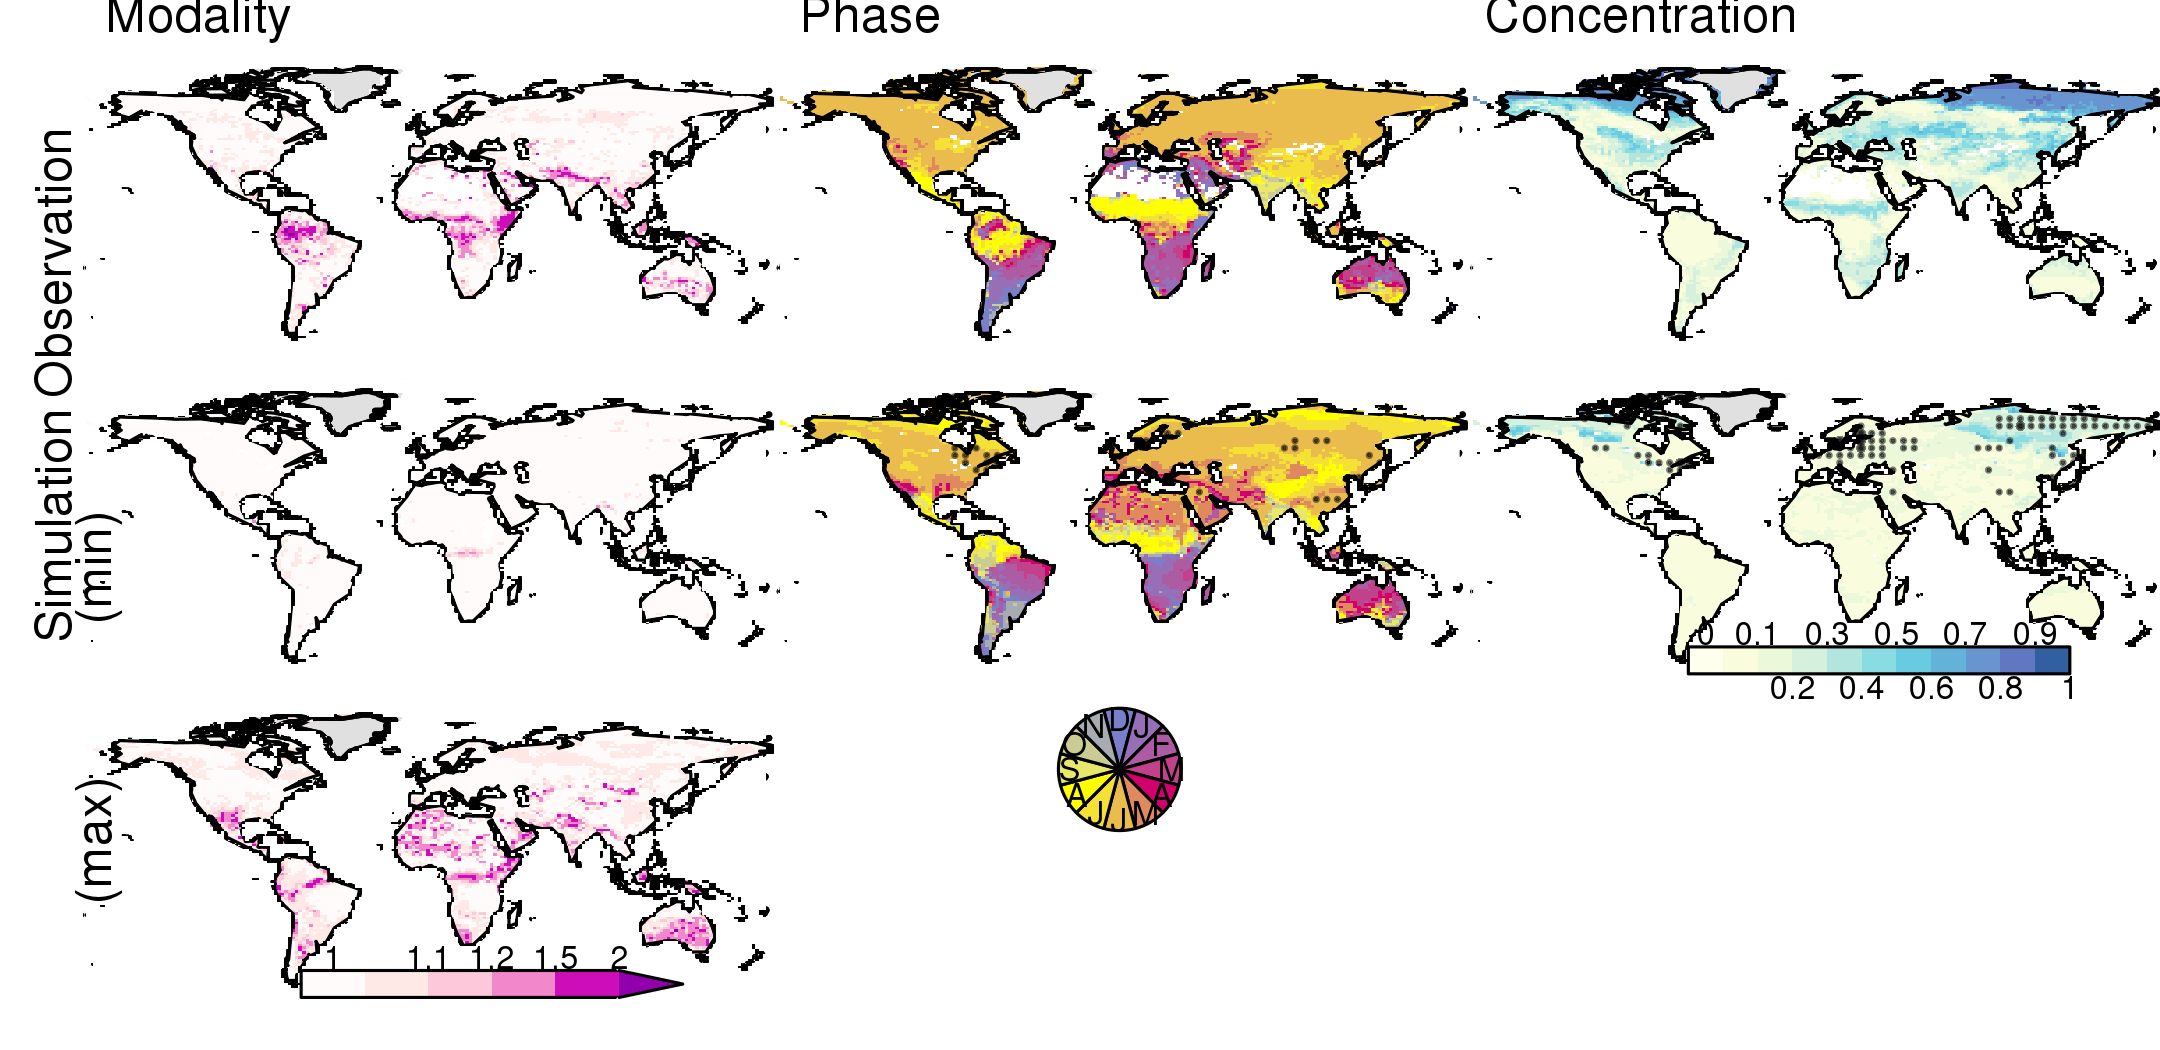
\includegraphics[width=12cm]{figs/LAI/fire_var_seasonality-maps-MPCcontrol-lai.png}
    \caption{Seasonal comparison for LAI \label{fig:LAIseasonalMap}}
\end{figure*}


\subsection{Carbon}
\hilight{Eddy - include fluxnet?}

\begin{itemize}
    \item Site-mean seasonal peak is not prolonged enough, dropping off too quickly in Jul-Sept. Seems to be an error in US sites.
    \item Spatial distribution of GPP is good. Too little in some tropical regions (inc. India), possibly related to climate (precip.) biases? To much in other tropical regions. Plots show obs, model, bias
    \item \hilight{Doug - remember to add veg distribution biases}
\end{itemize}

\subsubsection{Vegetation carbon}
\hilight{Eddy/Chantelle. Anything in iLamb?}
\hilight{Doug - use fireMIP stuff}

\subsubsection{Soil carbon}
\hilight{Eddy/Chantelle. Anything in iLamb?}

\subsubsection{GPP}
\begin{itemize}
    \item Too little in some tropical regions (inc. India), possibly related to climate (precip.) biases? To much in other tropical regions. Plots show obs, model, bias.
\end{itemize}

\begin{figure*}[t]
    %\begin{subfigure}
        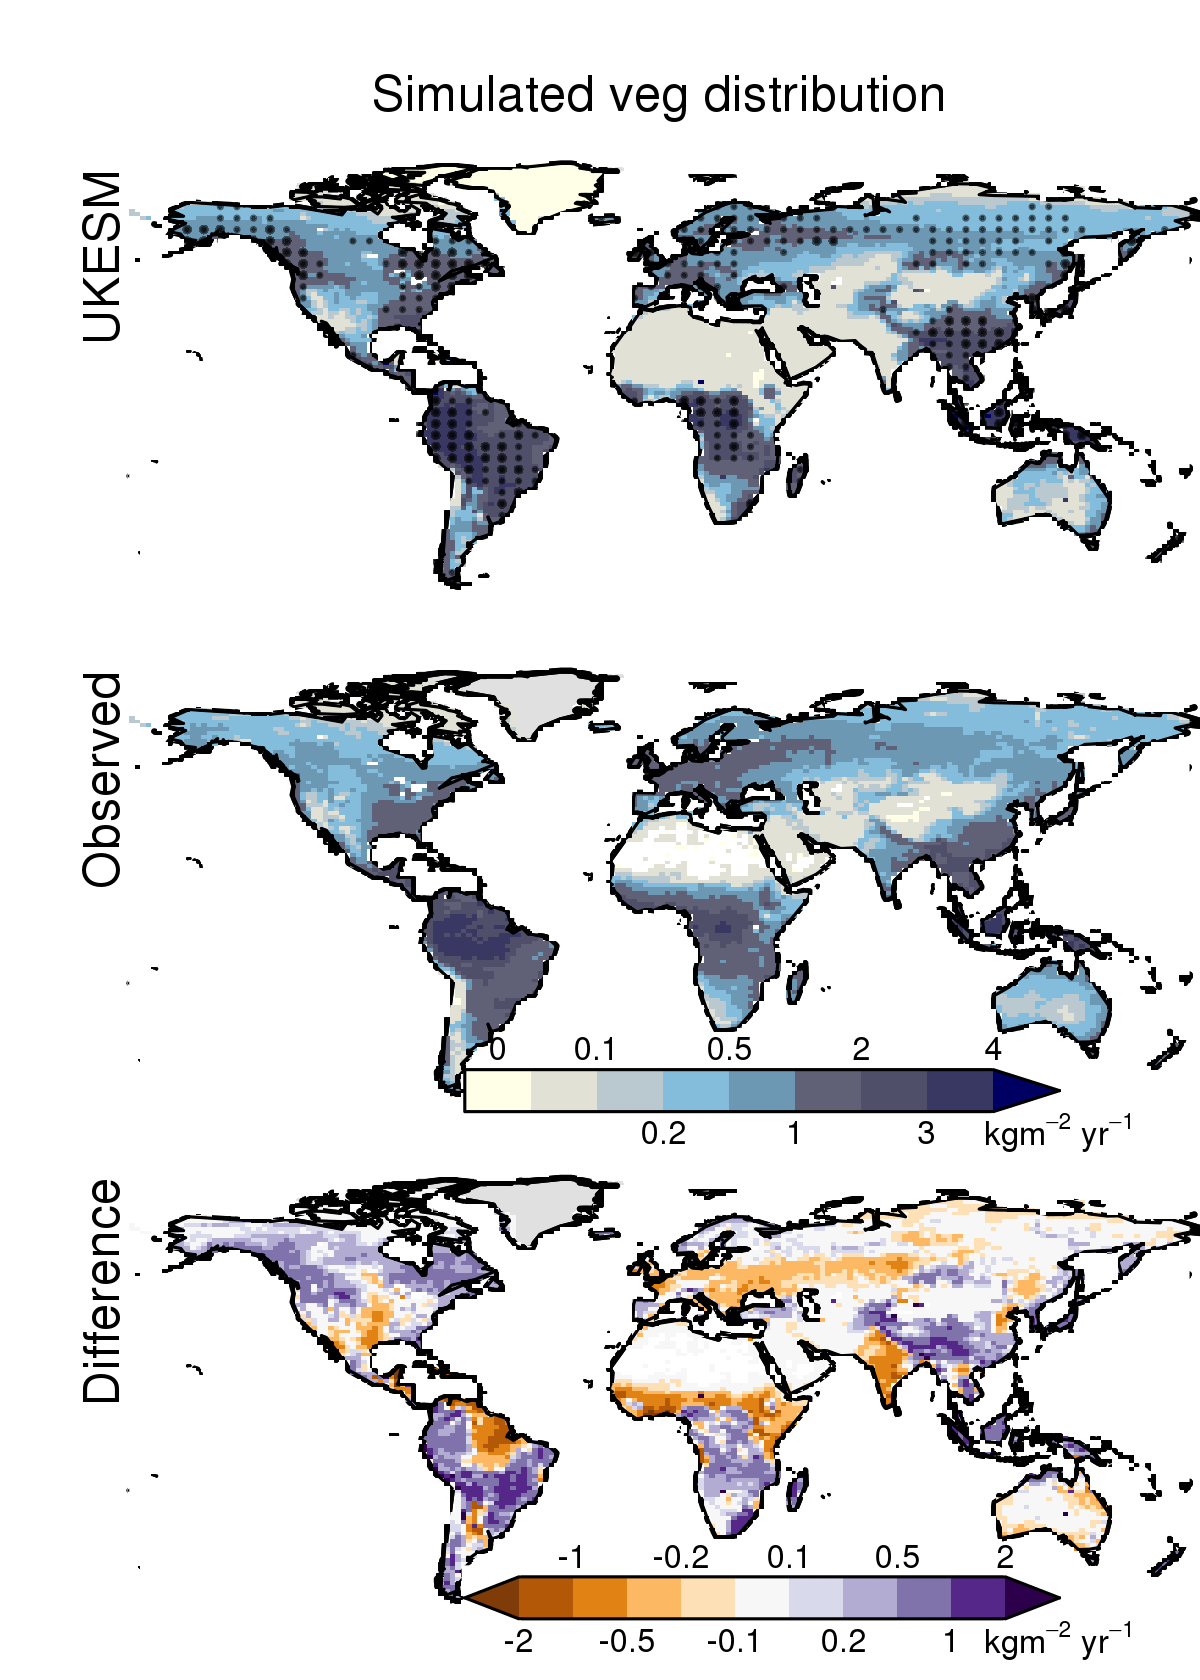
\includegraphics[width=5cm]{figs/GPP/fire_var_seasonality-maps-AA-mapscontrol-gpp.png}
    %\end{subfigure}
    %\begin{subfigure}
        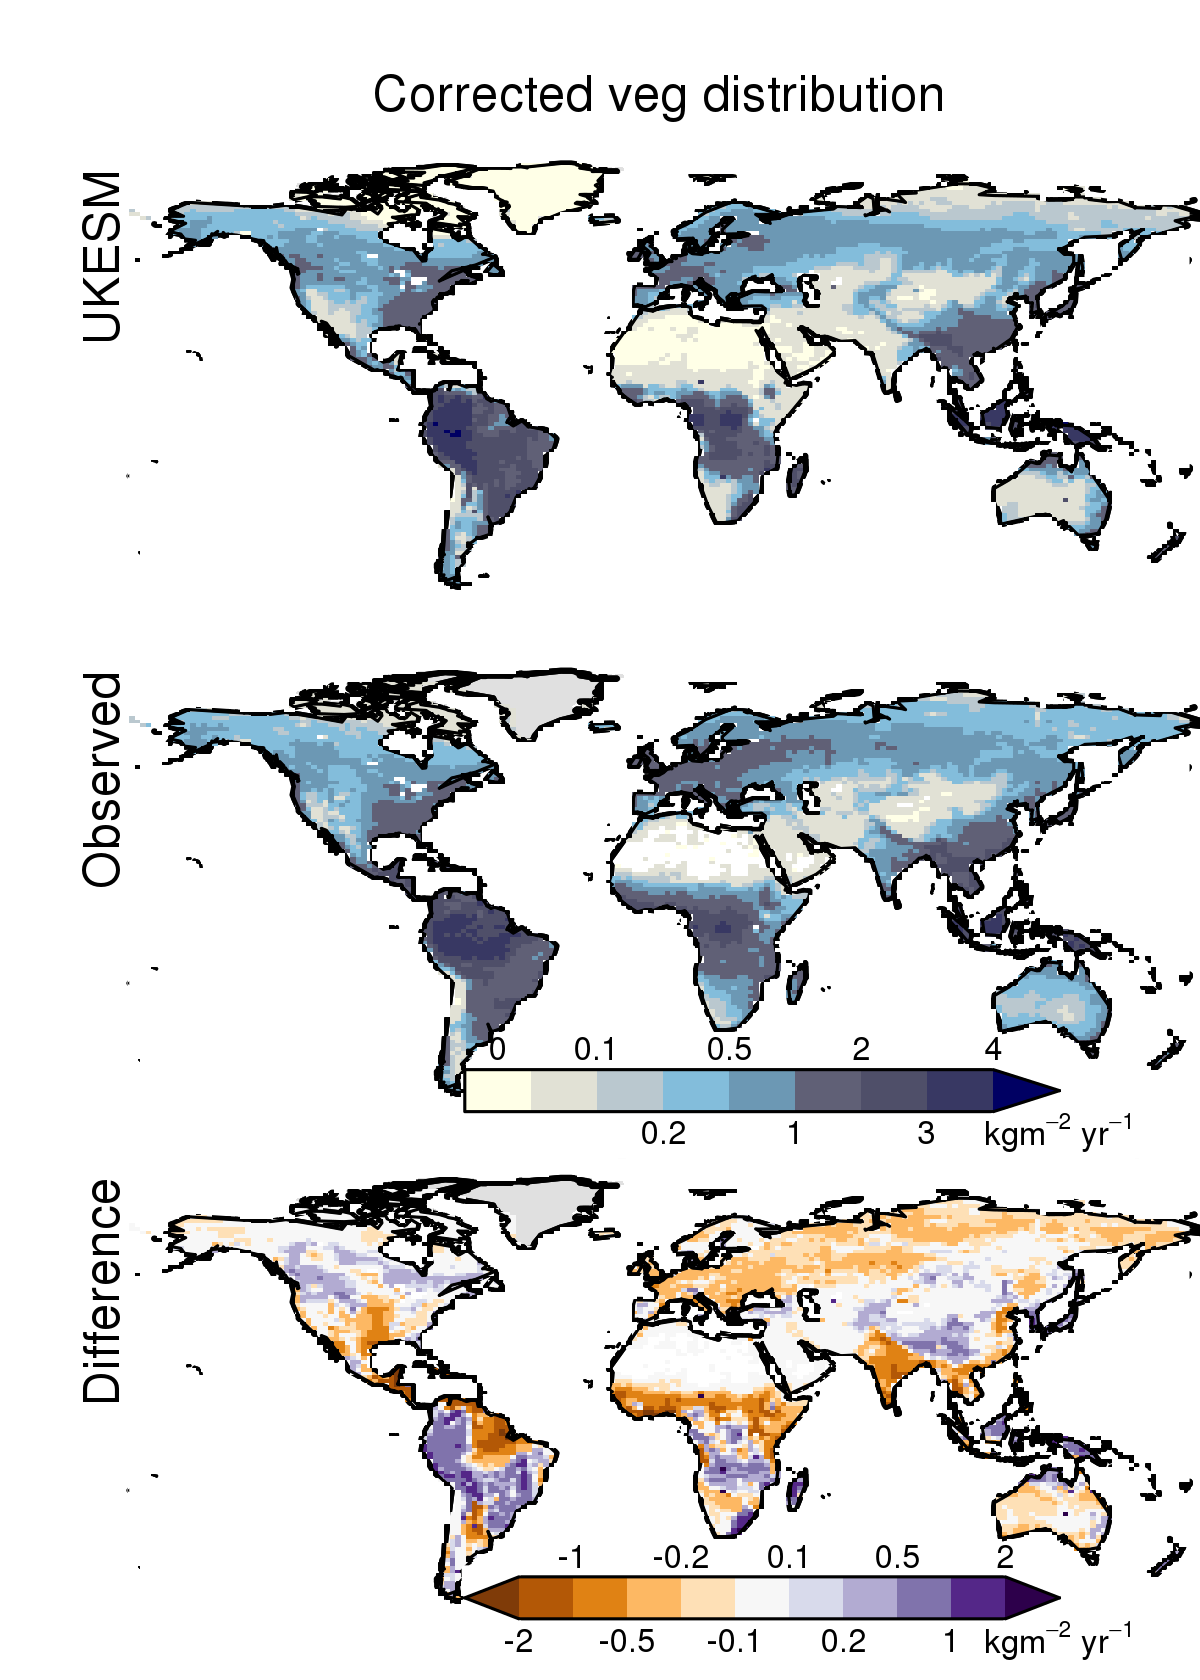
\includegraphics[width=5cm]{figs/GPP/fire_var_seasonality-maps-AA-mapsobsVegDist-gpp.png}
    
    %\end{subfigure}
    \caption{Simulated (top), observed (middle, <<ref>>) and different in mean annual GPP for 2001-2013. Right hand, UKESM has been corrected for vegetation distribution biases \label{fig:GPPmap}}
\end{figure*}

\begin{figure*}[t]
    %\begin{subfigure}
        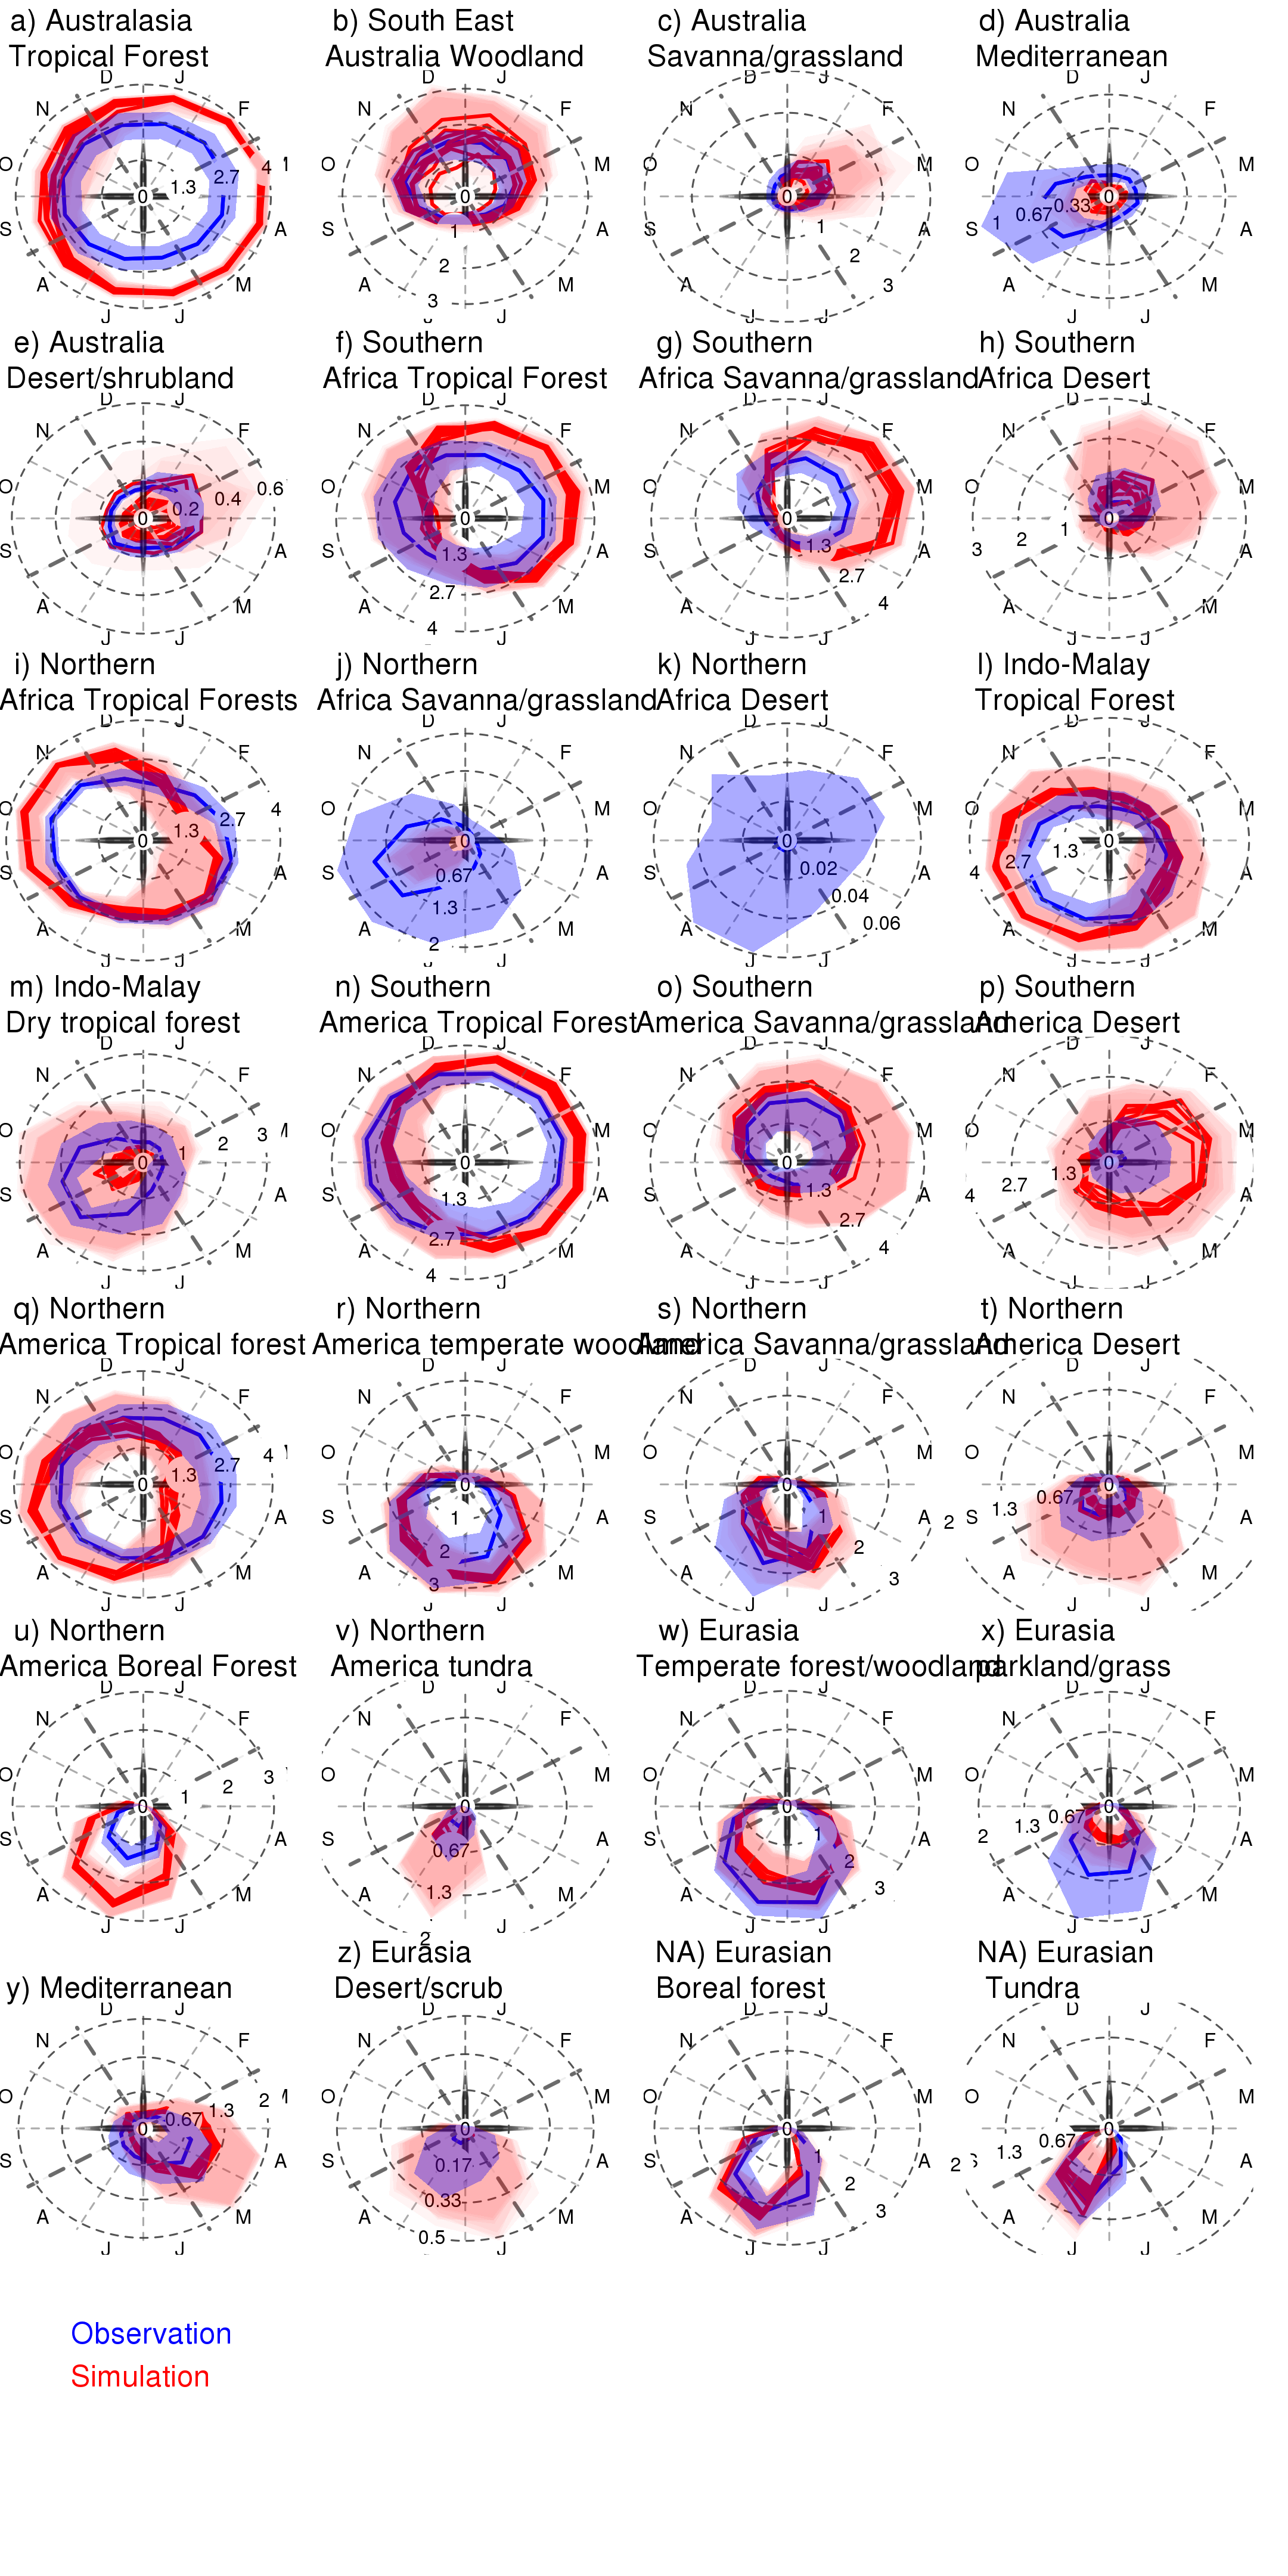
\includegraphics[width=5cm]{figs/GPP/fire_var_seasonality-TS-control-gpp.png}
    %\end{subfigure}
    %\begin{subfigure}
        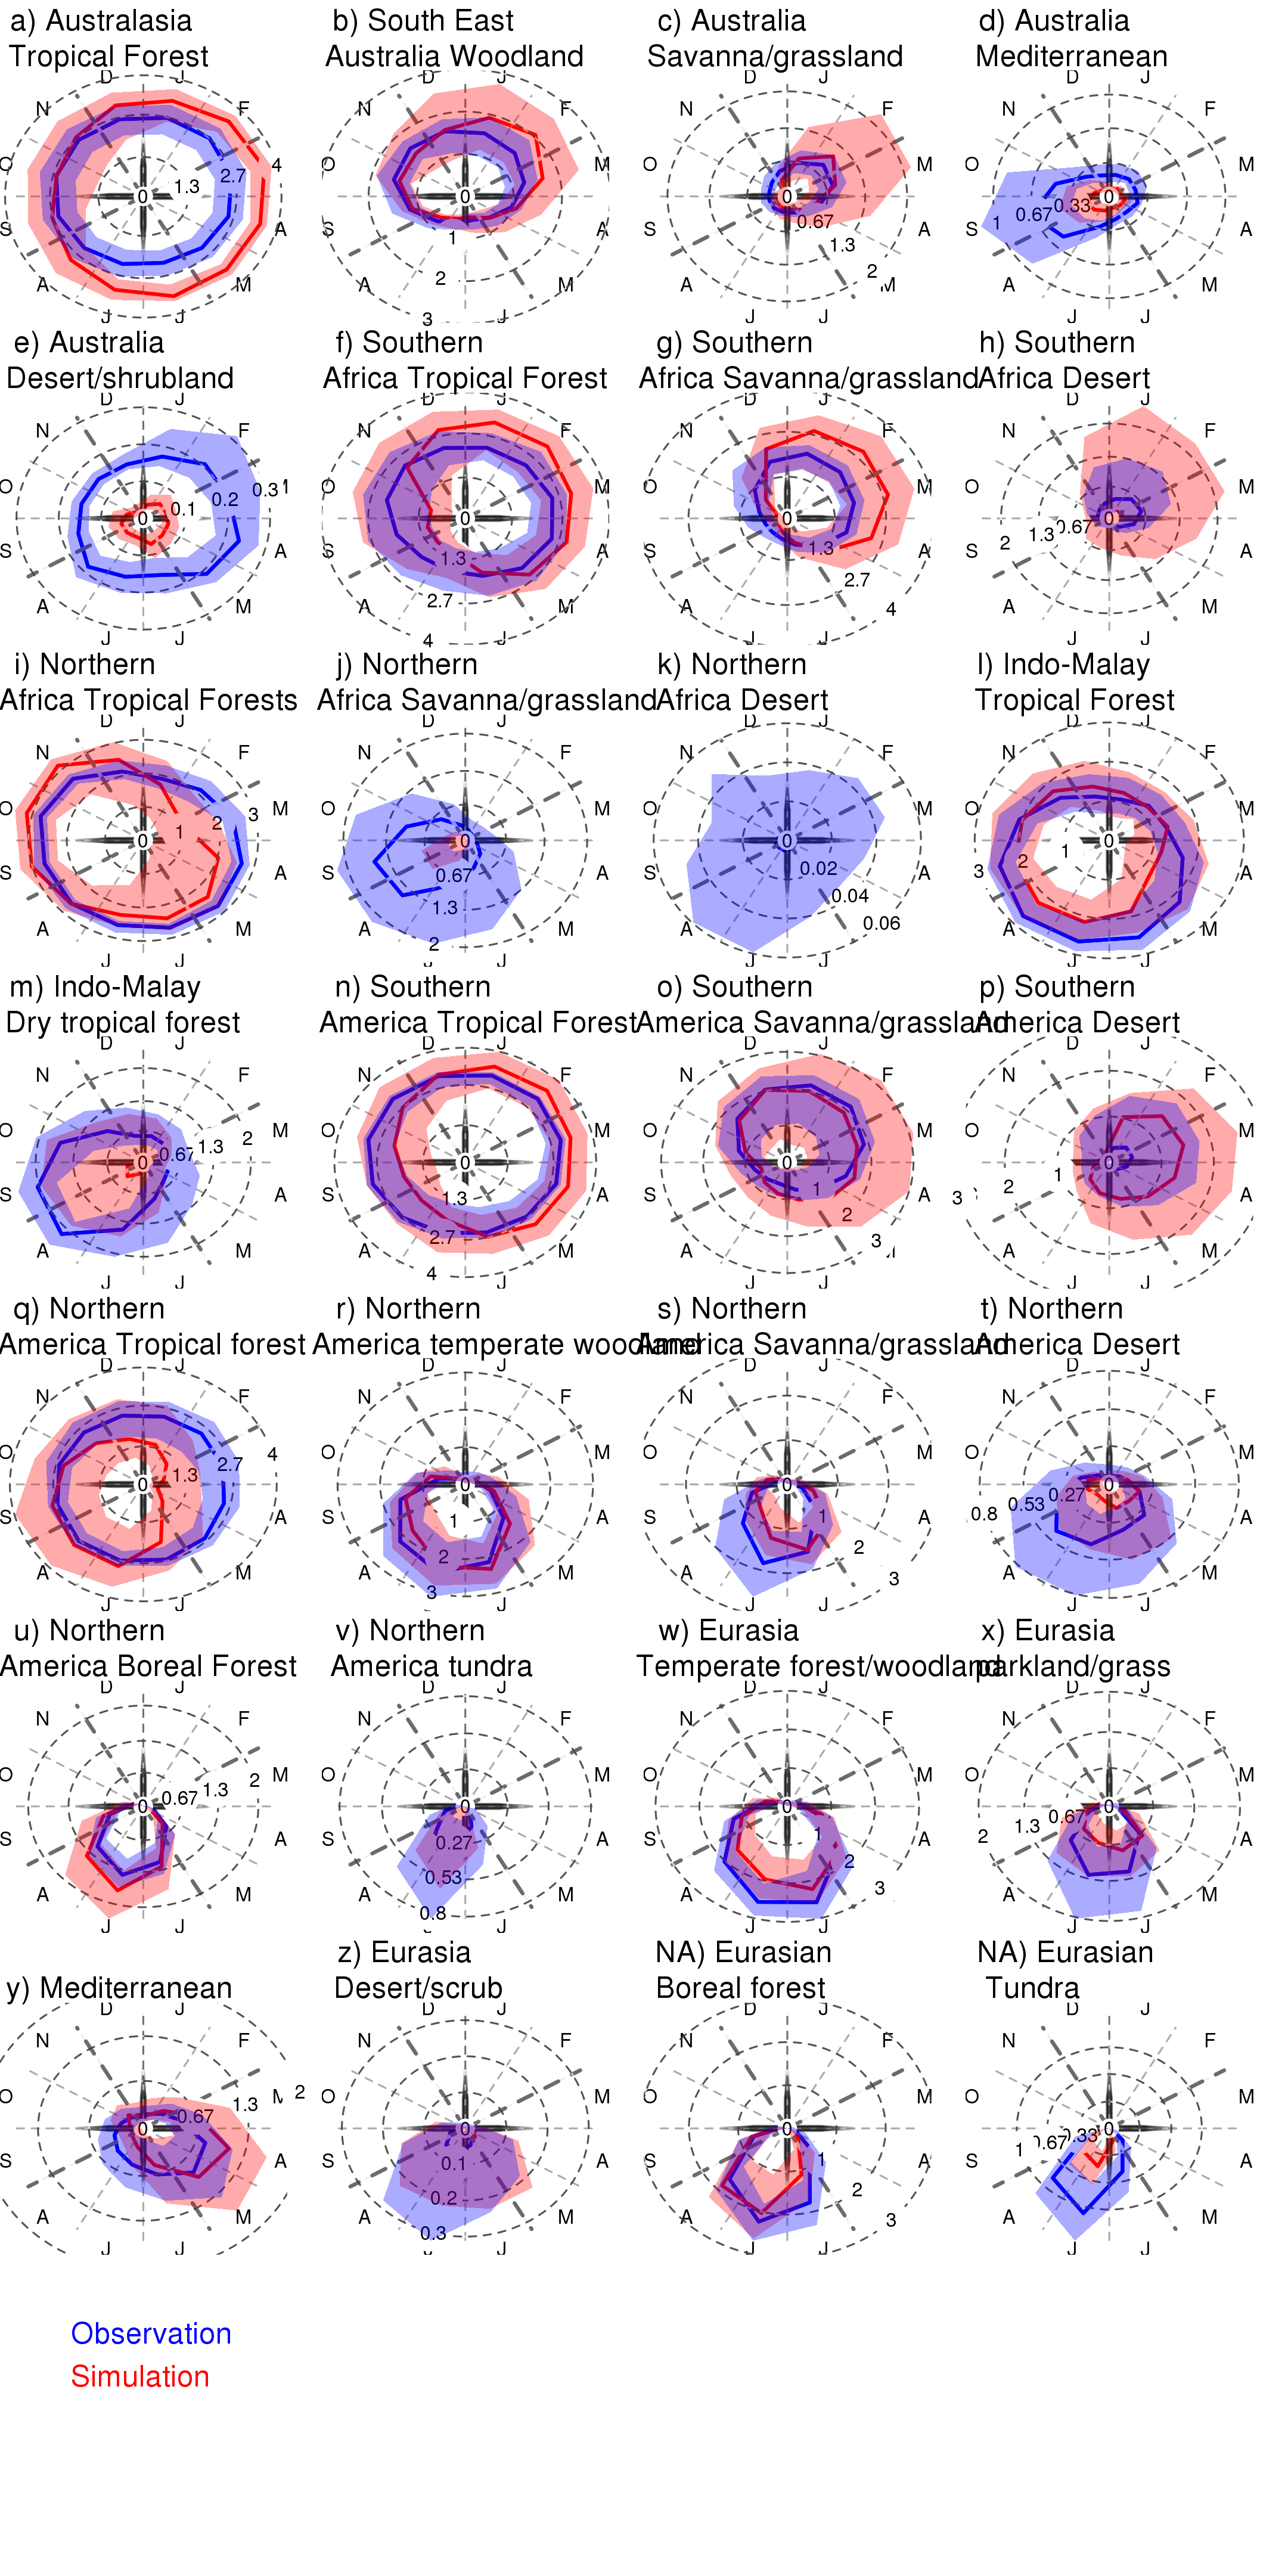
\includegraphics[width=5cm]{figs/GPP/fire_var_seasonality-TS-obsVegDist-gpp.png}
    
    %\end{subfigure}
    \caption{Simulated (red), observed (blue, <<ref>>) and seasonal cycles in GPP for 2001-2013 for each region(see \ref{fig:regionsMap}. Right hand, UKESM has been corrected for vegetation distribution biases \label{fig:GPPseasonalTS}}
\end{figure*}

\begin{figure*}[t]
    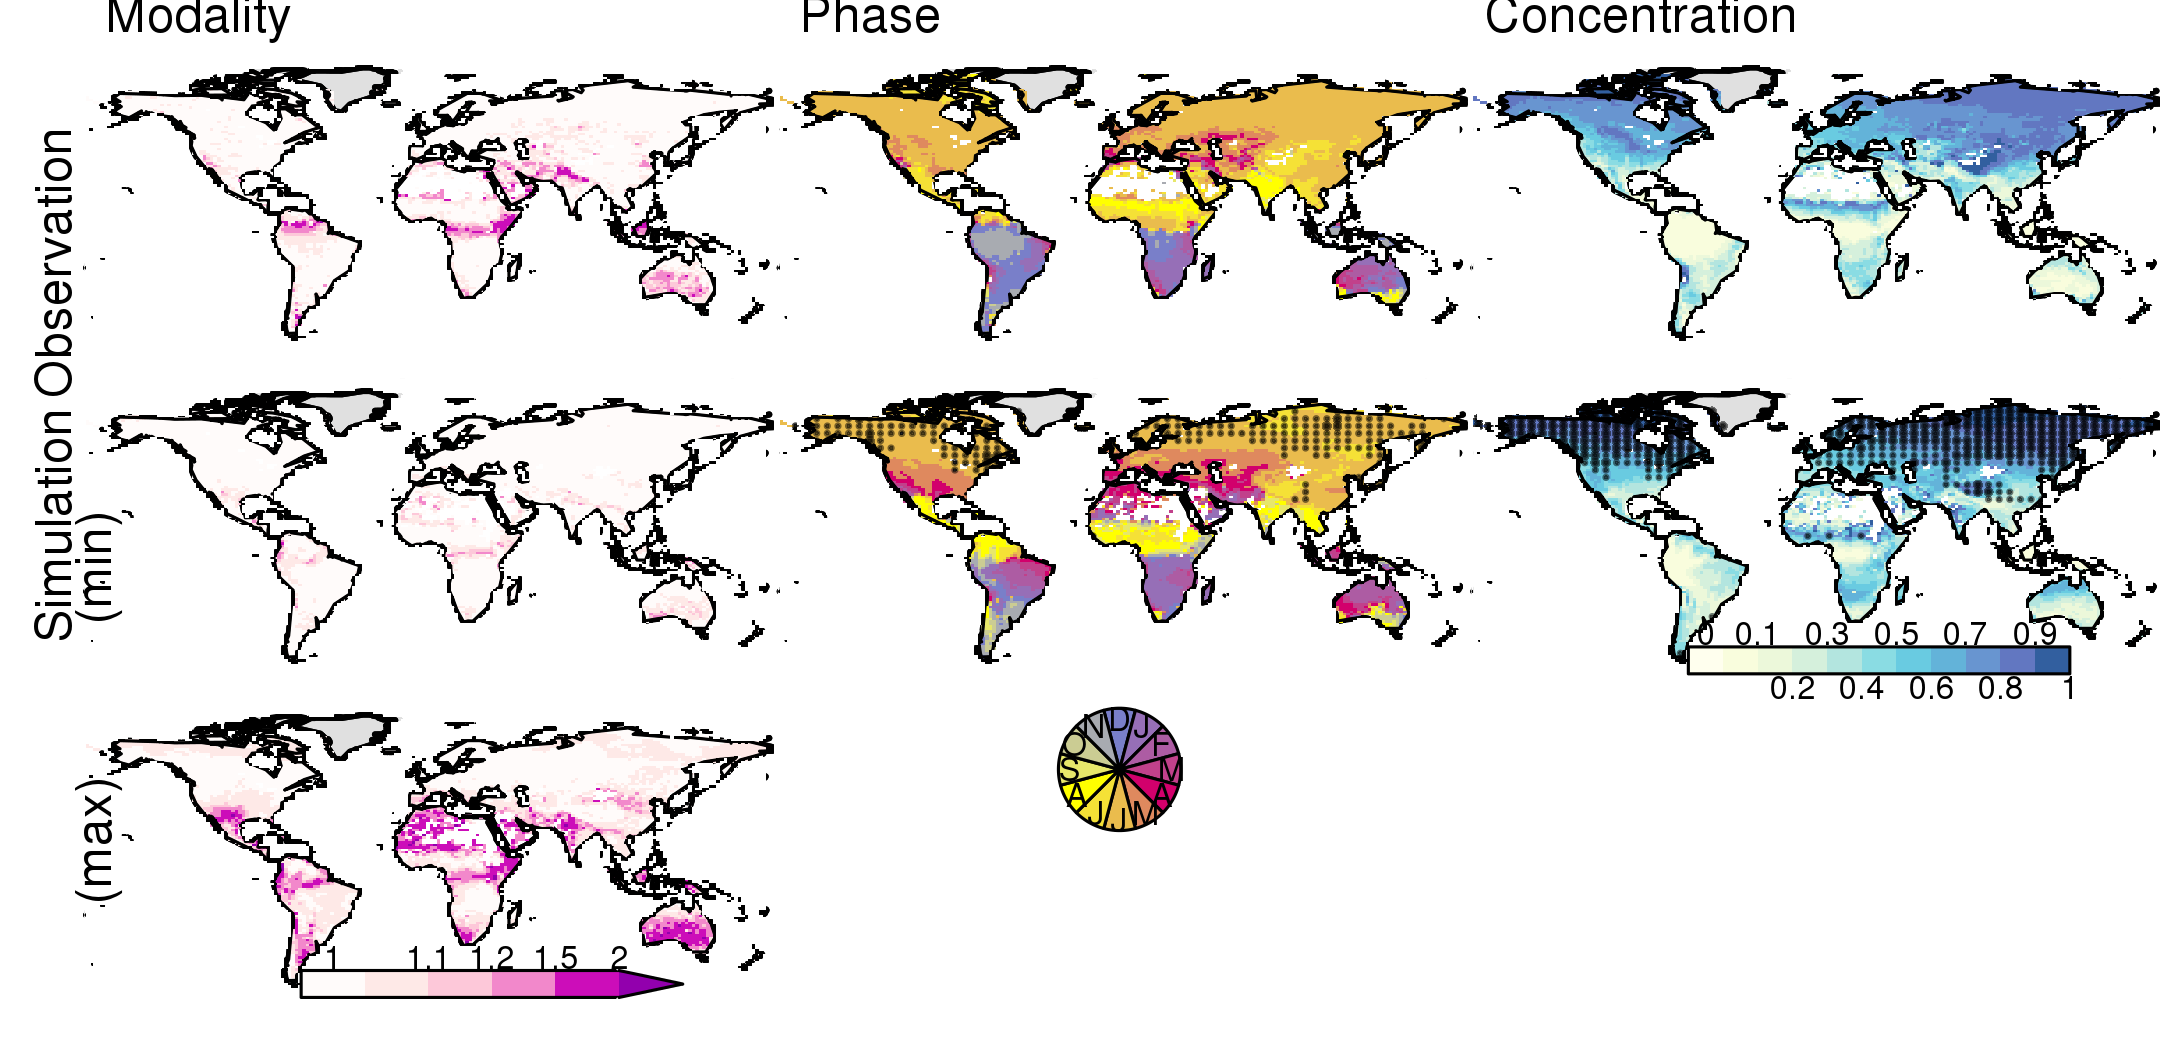
\includegraphics[width=12cm]{figs/GPP/fire_var_seasonality-maps-MPCcontrol-gpp.png}
    \caption{Seasonal comparison for GPP \label{fig:GPPseasonalMap}}
\end{figure*}


\subsubsection{Carbon turnover}
\hilight{Rebecca V - summary of results}

\begin{itemize}

	\item Globally the spatial pattern of both ecosystem carbon turnover and soil carbon turnover is reasonably well matched in UKESM1-0-LL compared with observations, which can be seen in the Figures `ecosystem tau map' and `soil tau map' respectively; however there is a bias towards longer turnover times in UKESM1-0-LL compared with the observational data. There are regions in the northern mid-latitudes which have noticeably long turnover times in UKESM1-0-LL, which is not seen in the observational figure. This seems to be due to corresponding large quantities of soil carbon seen in these regions, which again is not seen in the observational figure.This could be due to cSoil being related to vegetation or due to nitrogen decomposition? However, we note that globally the soil carbon turnover times in UKESM1-0-LL better match the observational data compared with the ecosystem carbon turnover times. In regions of the Northern latitudes, UKESM1-0-LL produces very long ecosystem turnover times which are greater than the corresponding soil carbon turnover times. This is likely to be a result of not an accurate representation of high latitude vegetation.
	
	\item We investigated the spatial sensitivity of both ecosystem carbon turnover ($\tau_\mathrm{e}$), and soil carbon turnover ($\tau_\mathrm{s}$) to temperature and precipitation, which can be seen in Figures `ecosystem tau scatterplot' and `soil tau scatterplot' respectively. These sensitivities were considered on a global scale and for the different biomes considered in this study (Tropical Evergreen Forest, Temperate Forest, Grassland, Mediterranean, Desert, Boreal Forest, Tundra). In all cases, spatial data (latitude / longitude) was plotted as follows: precipitation (y-axis) against temperature (x-axis), and then the data was coloured by the respective turnover, $\tau_\mathrm{e}$ and $\tau_\mathrm{s}$, values (colour bar). Globally the spatial pattern of the sensitivity of $\tau_\mathrm{e}$ and $\tau_\mathrm{s}$ to temperature and precipitation is reproduced in UKESM1-0-LL compared with observations. We investigate these sensitivities in individual biomes to locate where UKESM1-0-LL accurately matched observations, and where there are differences and model improvements are required.
	
	\item In the Tropical Evergreen Forest biome, UKESM1-0-LL matches well with the observations, with only a marginally slower turnover in observations. In Figure `ecosystem tau scatterplot' it can be seen that there are points with unusually long ecosystem carbon turnover times, which is likely to be due to the vegetation allocation in this biome.
	
	\item In the Grassland and Temperate Forest biomes, for both $\tau_\mathrm{e}$ and $\tau_\mathrm{s}$, UKESM1-0-LL generally has longer turnover times compared with observations. This could potentially be due to vegetation disturbances, UKESM1-0-LL is known to have harsh vegetation transitions, which might be causing no vegetation to be growing in some regions. Additionally, for both $\tau_\mathrm{e}$ and $\tau_\mathrm{s}$, there seems to be more of a temperature relationship to turnover seen in this biome in UKESM1-0-LL compared with the observations, whereas in observations there is more of a sensitivity to precipitation.
	
	\item In the Mediterranean biome, UKESM1-0-LL does not match the temperature and precipitation relationships to $\tau_\mathrm{e}$ and $\tau_\mathrm{s}$ as seen in observations. In the observations, lower precipitation and higher temperature results in a longer carbon turnover, whereas the opposite affect is seen in UKESM1-0-LL.
	
	\item The Desert and Boreal Forest biomes are exceptions where UKESM1-0-LL does not produce slower carbon turnover compared with observations. In the Desert biome, a stronger temperature sensitivity on carbon turnover is seen in UKESM1-0-LL compared with observations, whereas a stronger precipitation sensitivity is seen in observations. This precipitation sensitivity is partly seen for $\tau_\mathrm{s}$, however is not seen at all for $\tau_\mathrm{e}$, which means it is likely to be due to wrong vegetation here? In the Boreal Forest biome, long carbon turnover times are seen in the observations, with a sensitivity to temperature within the biome, both of these are not seen in UKESM1-0-LL. Within UKESM1-0-LL, there is a slight precipitation sensitivity seen in this biome, though less variation in turnover is seen compared to observations.

	\item In the Tundra biome however, a greater variation of turnover is seen within the biome in UKESM1-0-LL compared with observations, due to a more apparent temperature sensitivity of turnover in UKESM1-0-LL. Again, this could be due to not an accurate representation of high latitude vegetation.
	
	\item \textit{We note our results are dependent on the choice of benchmark observational datasets (cite tau uncertainty paper).}

\end{itemize}



\begin{figure*}[t]
    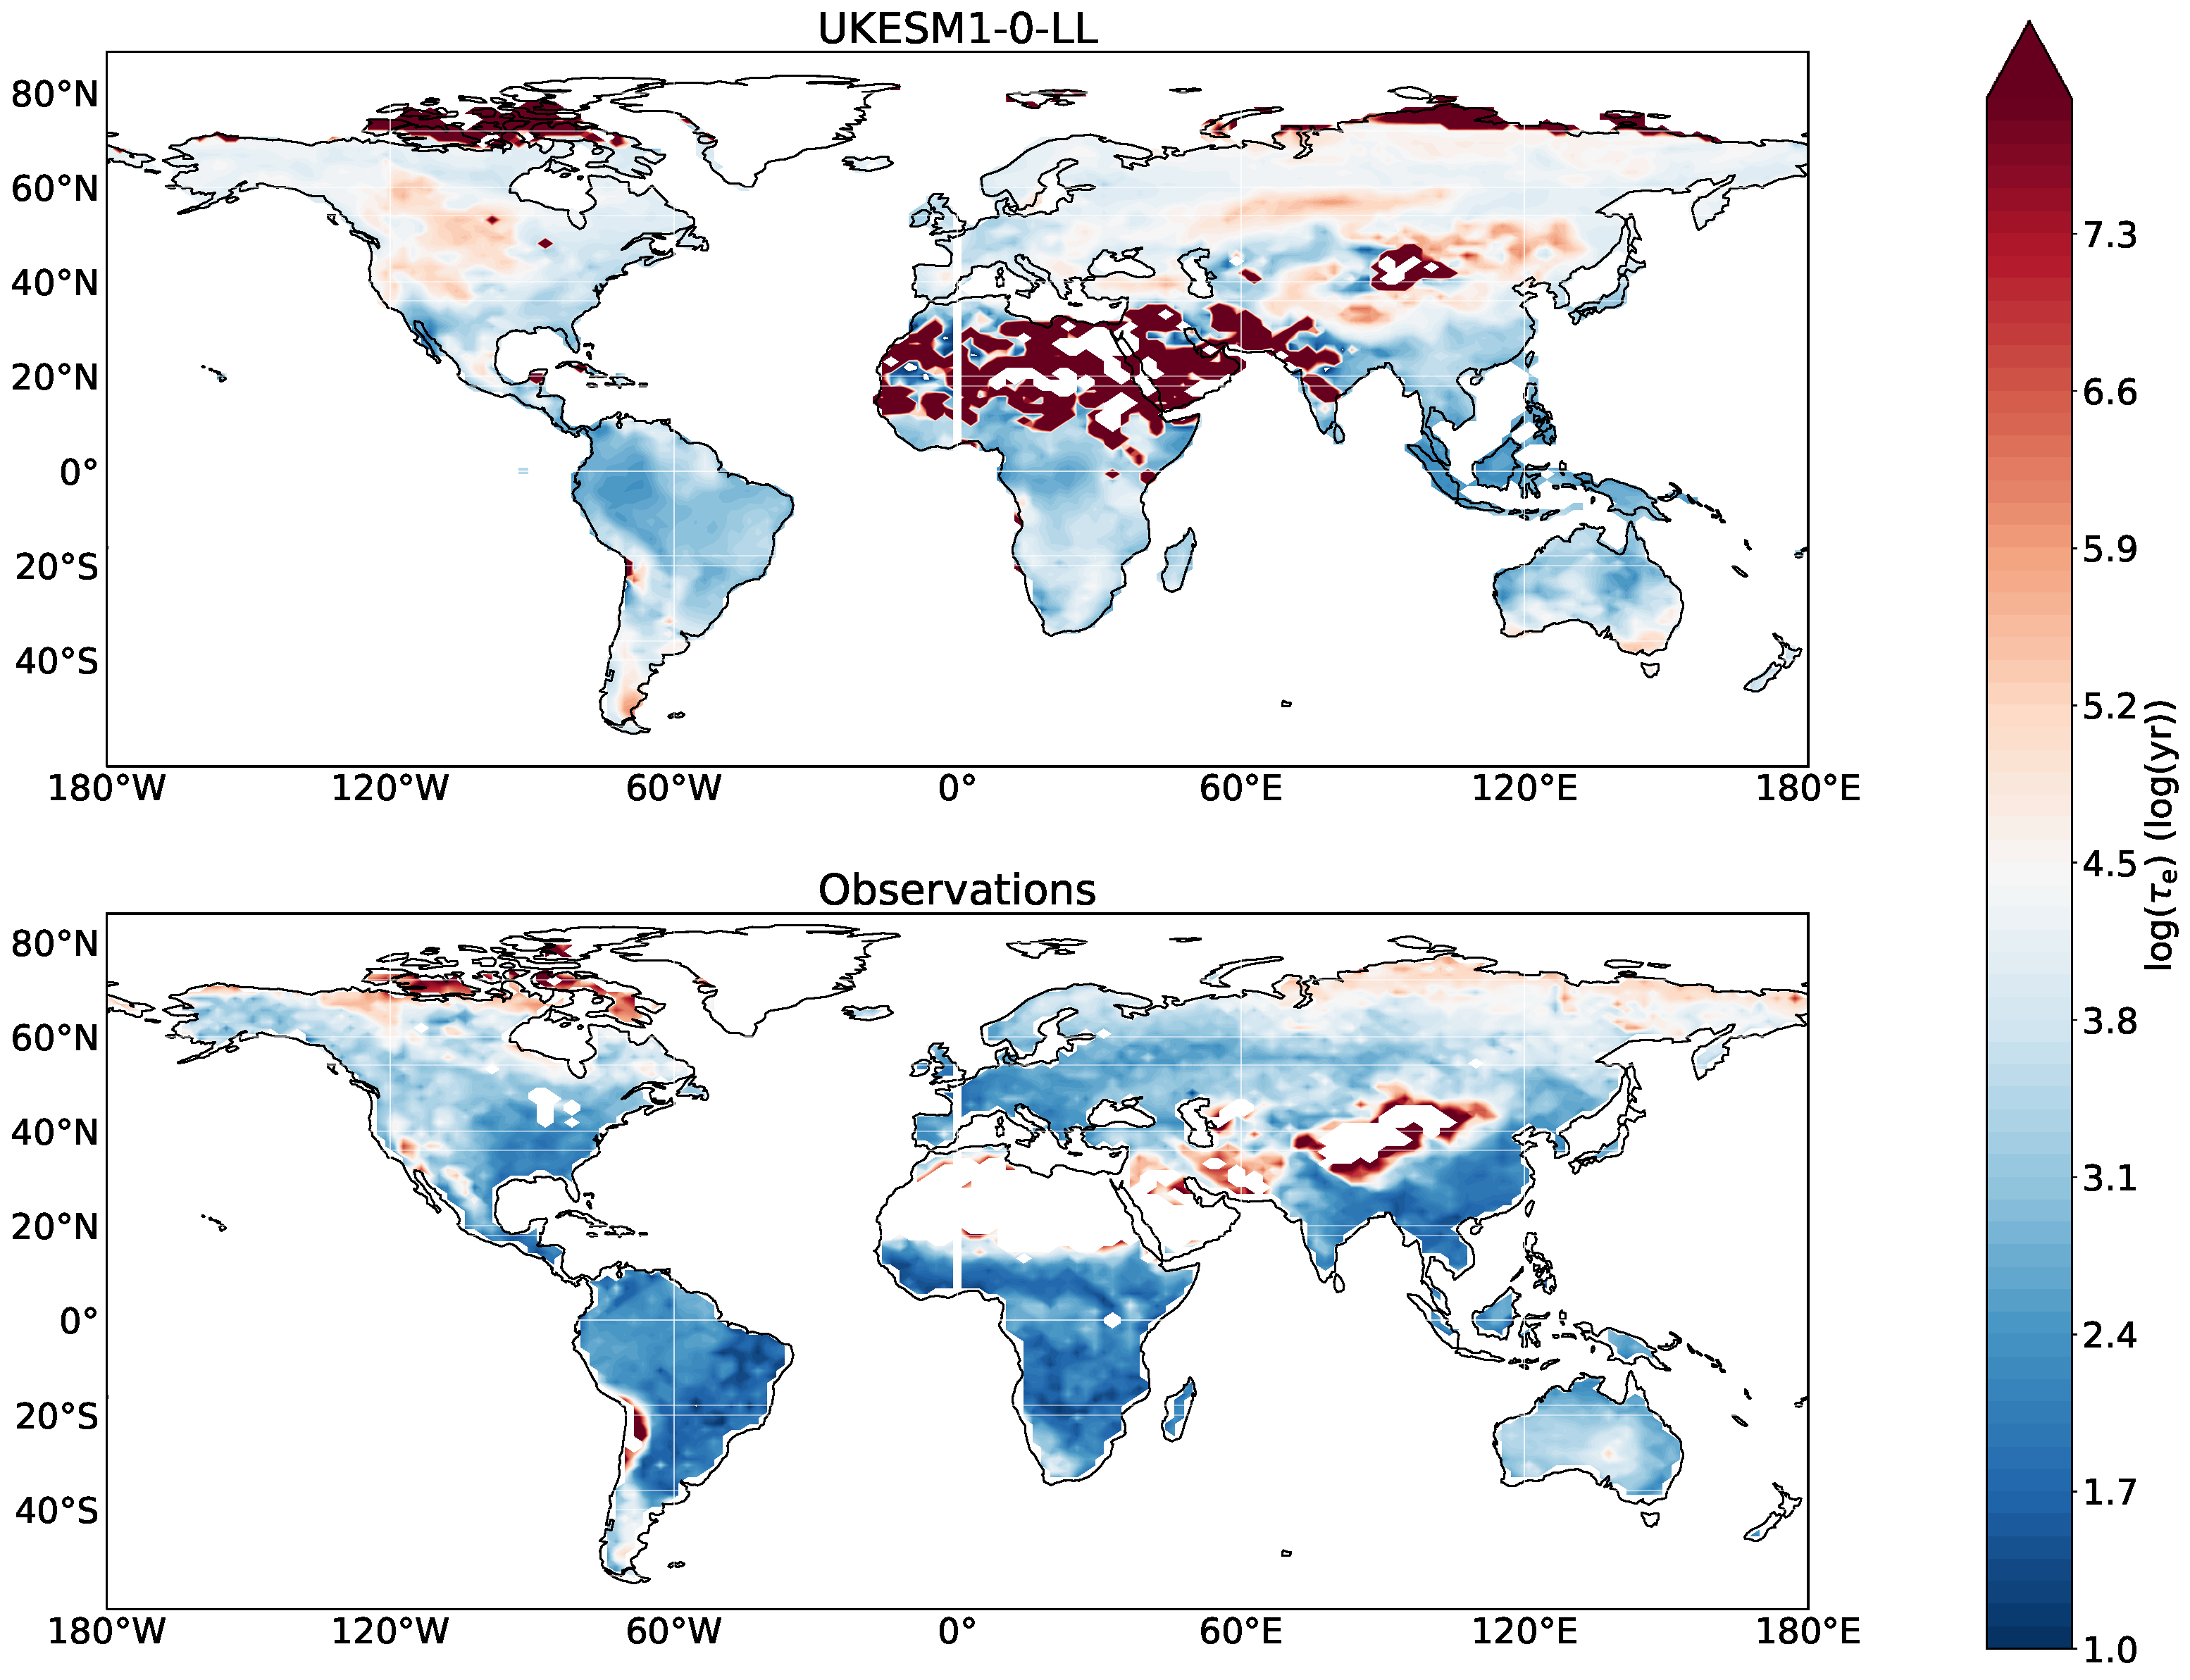
\includegraphics[width=12cm]{figs/Turnover/ecosystem_tau_map_comparison.pdf}
    \caption{Ecosystem turnover \label{fig:EcoTurnoverlMap}}
\end{figure*}

\begin{figure*}[t]
    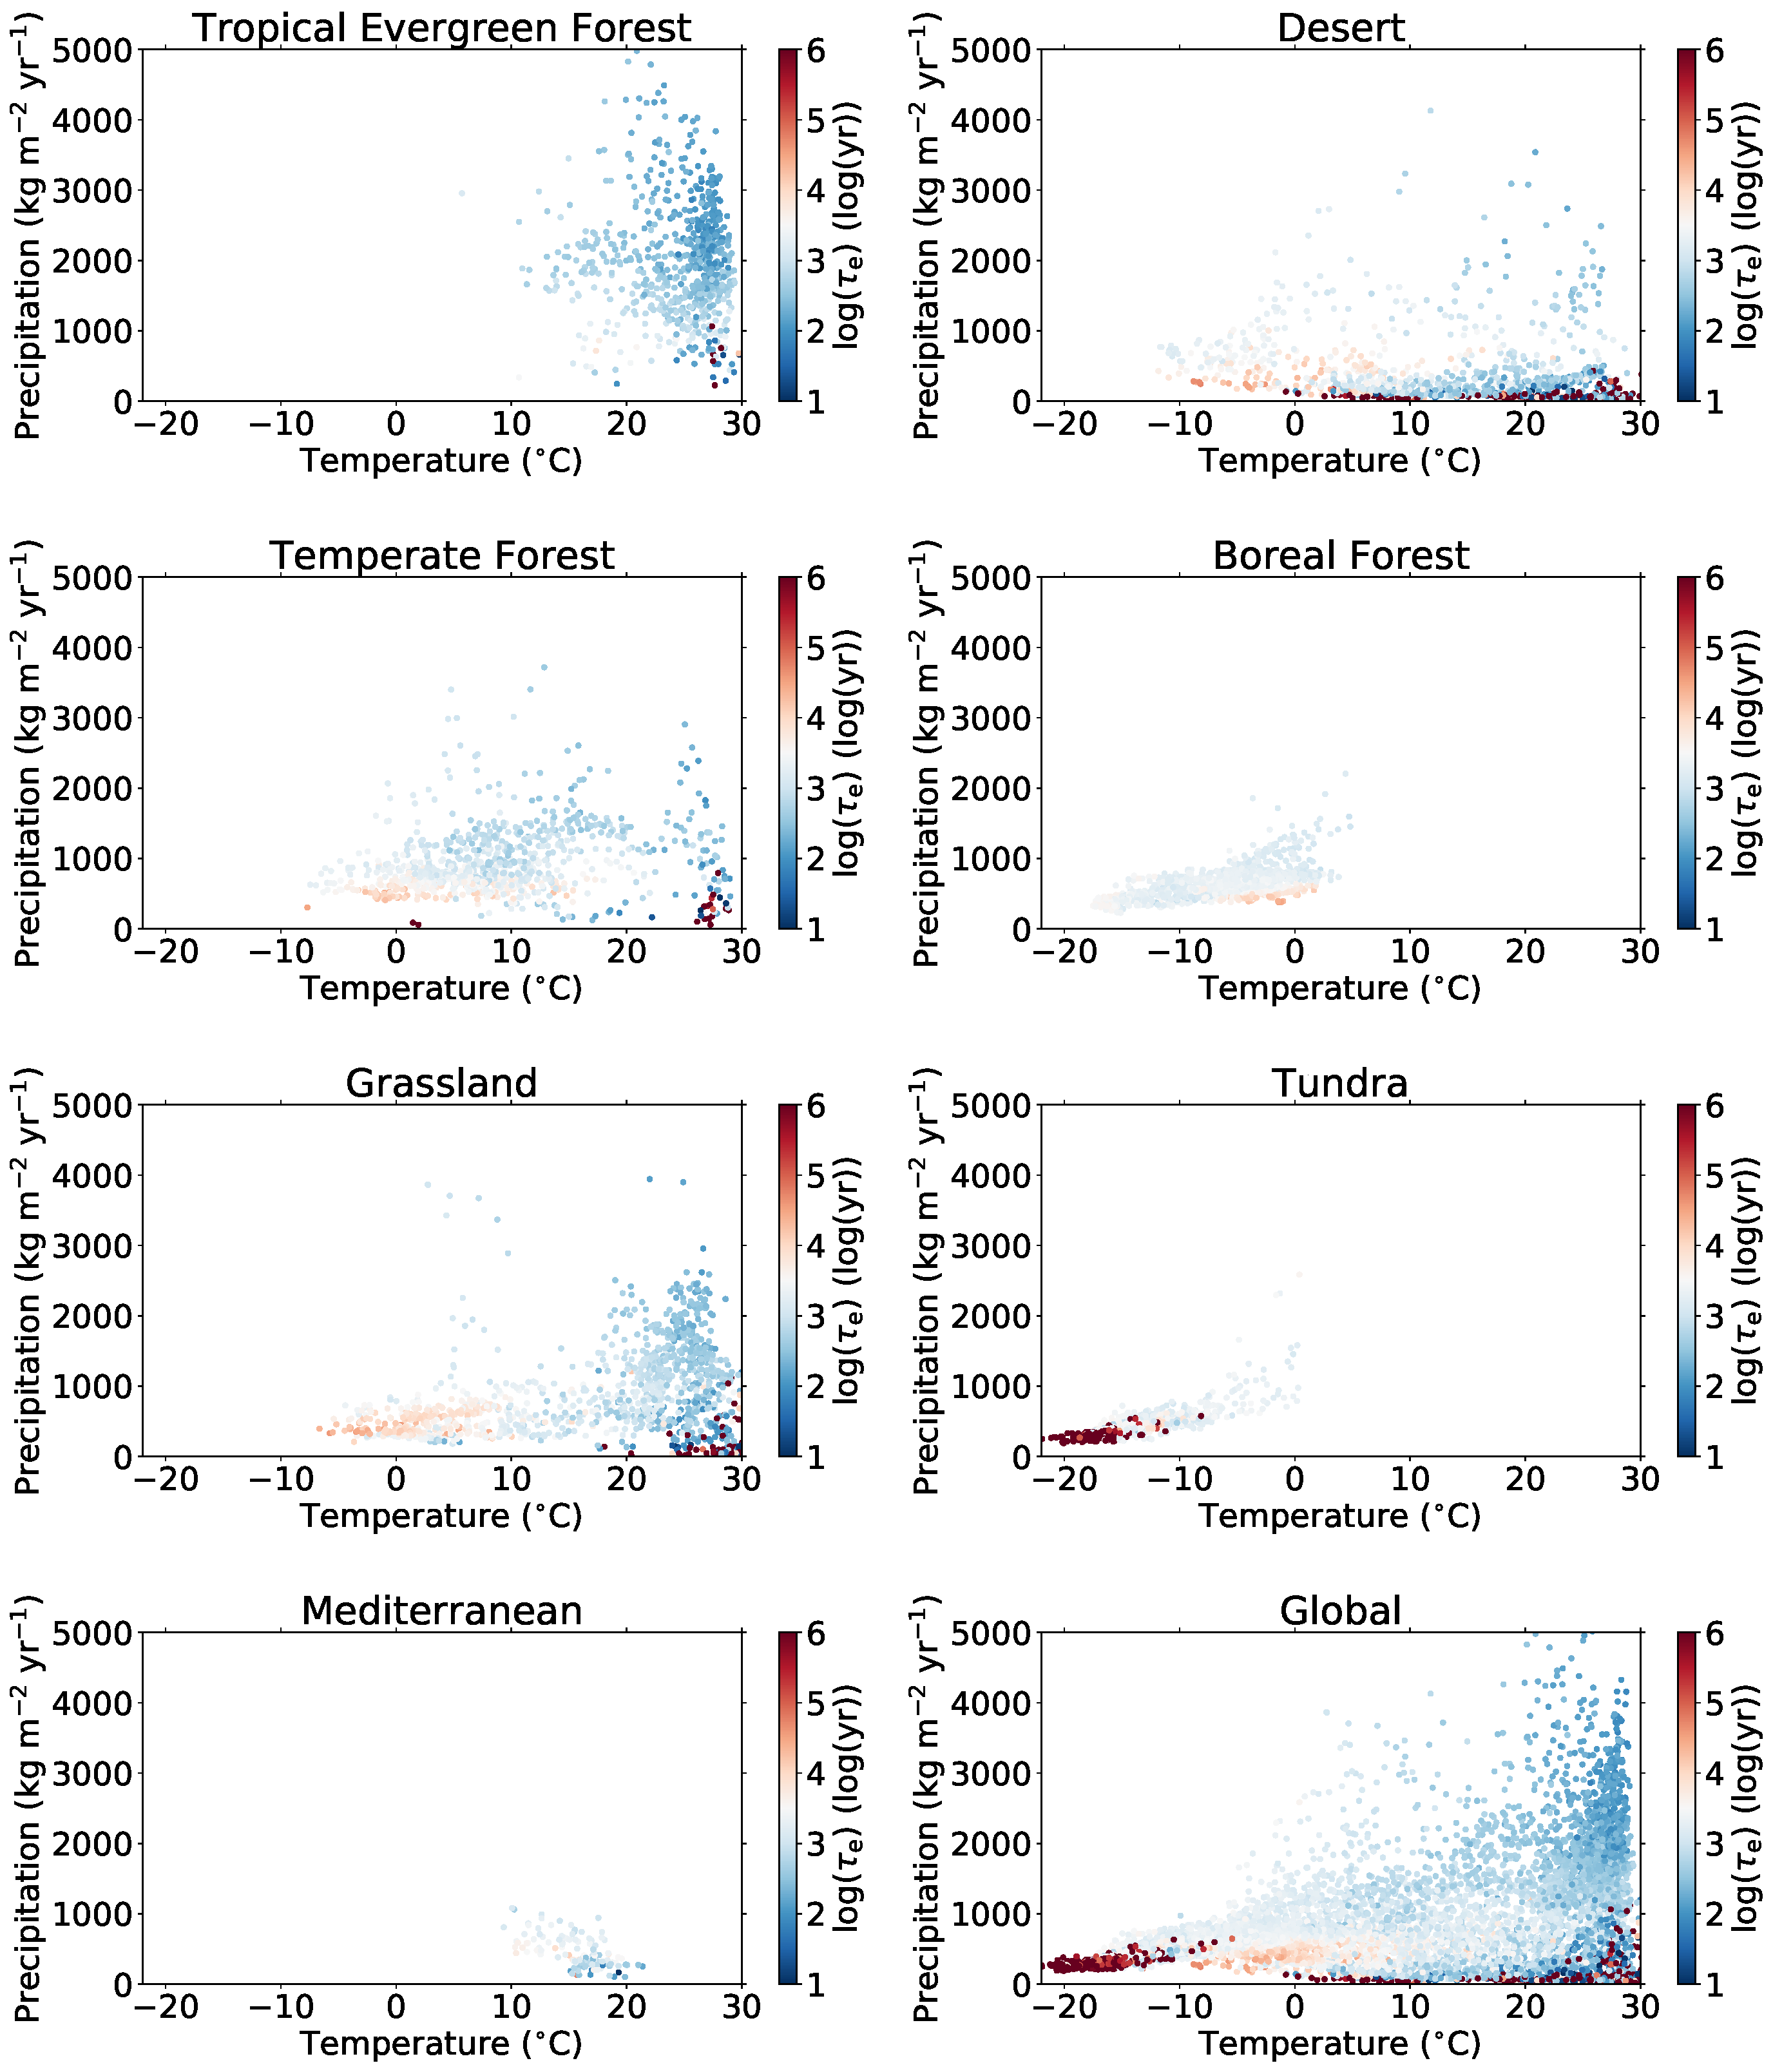
\includegraphics[width=6cm]{figs/Turnover/UKESM_ecosystem_colouredbytau_biome_log.pdf}
    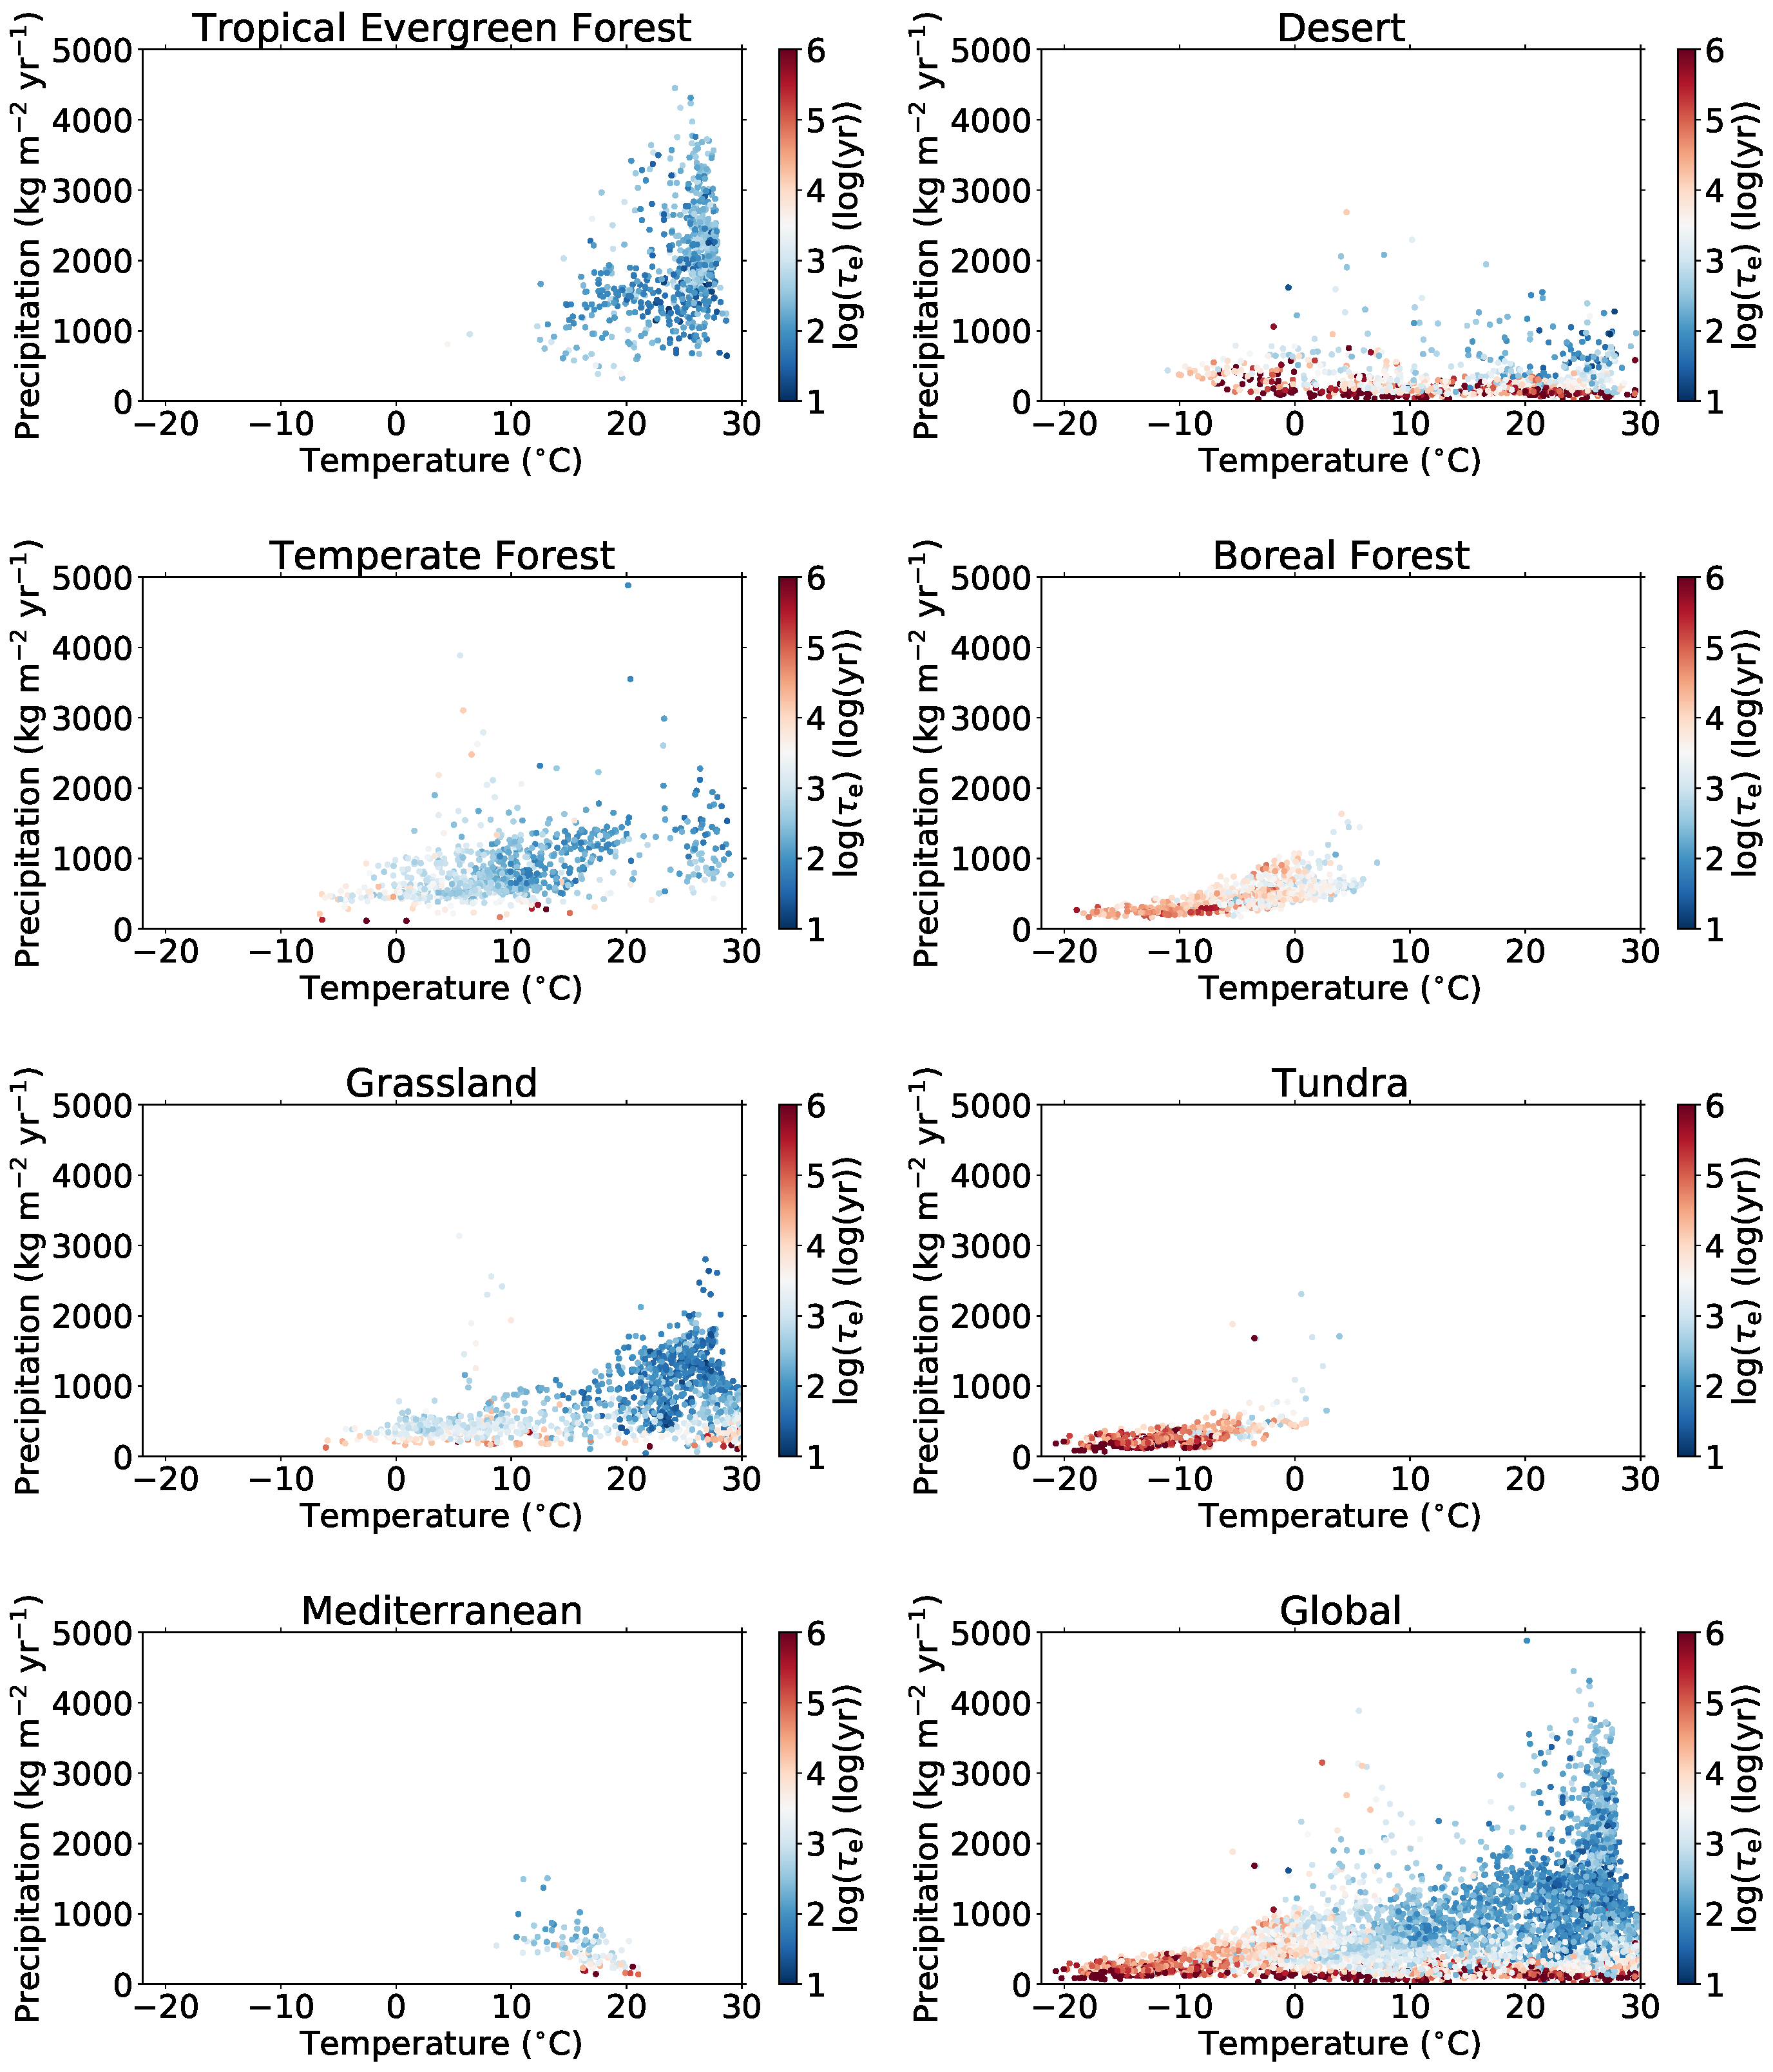
\includegraphics[width=6cm]{figs/Turnover/obs1_ecosystem_colouredbytau_biome_log.pdf}
    \caption{Ecosystem turnover \label{fig:EcoTurnoverScatter}}
\end{figure*}

\begin{figure*}[t]
    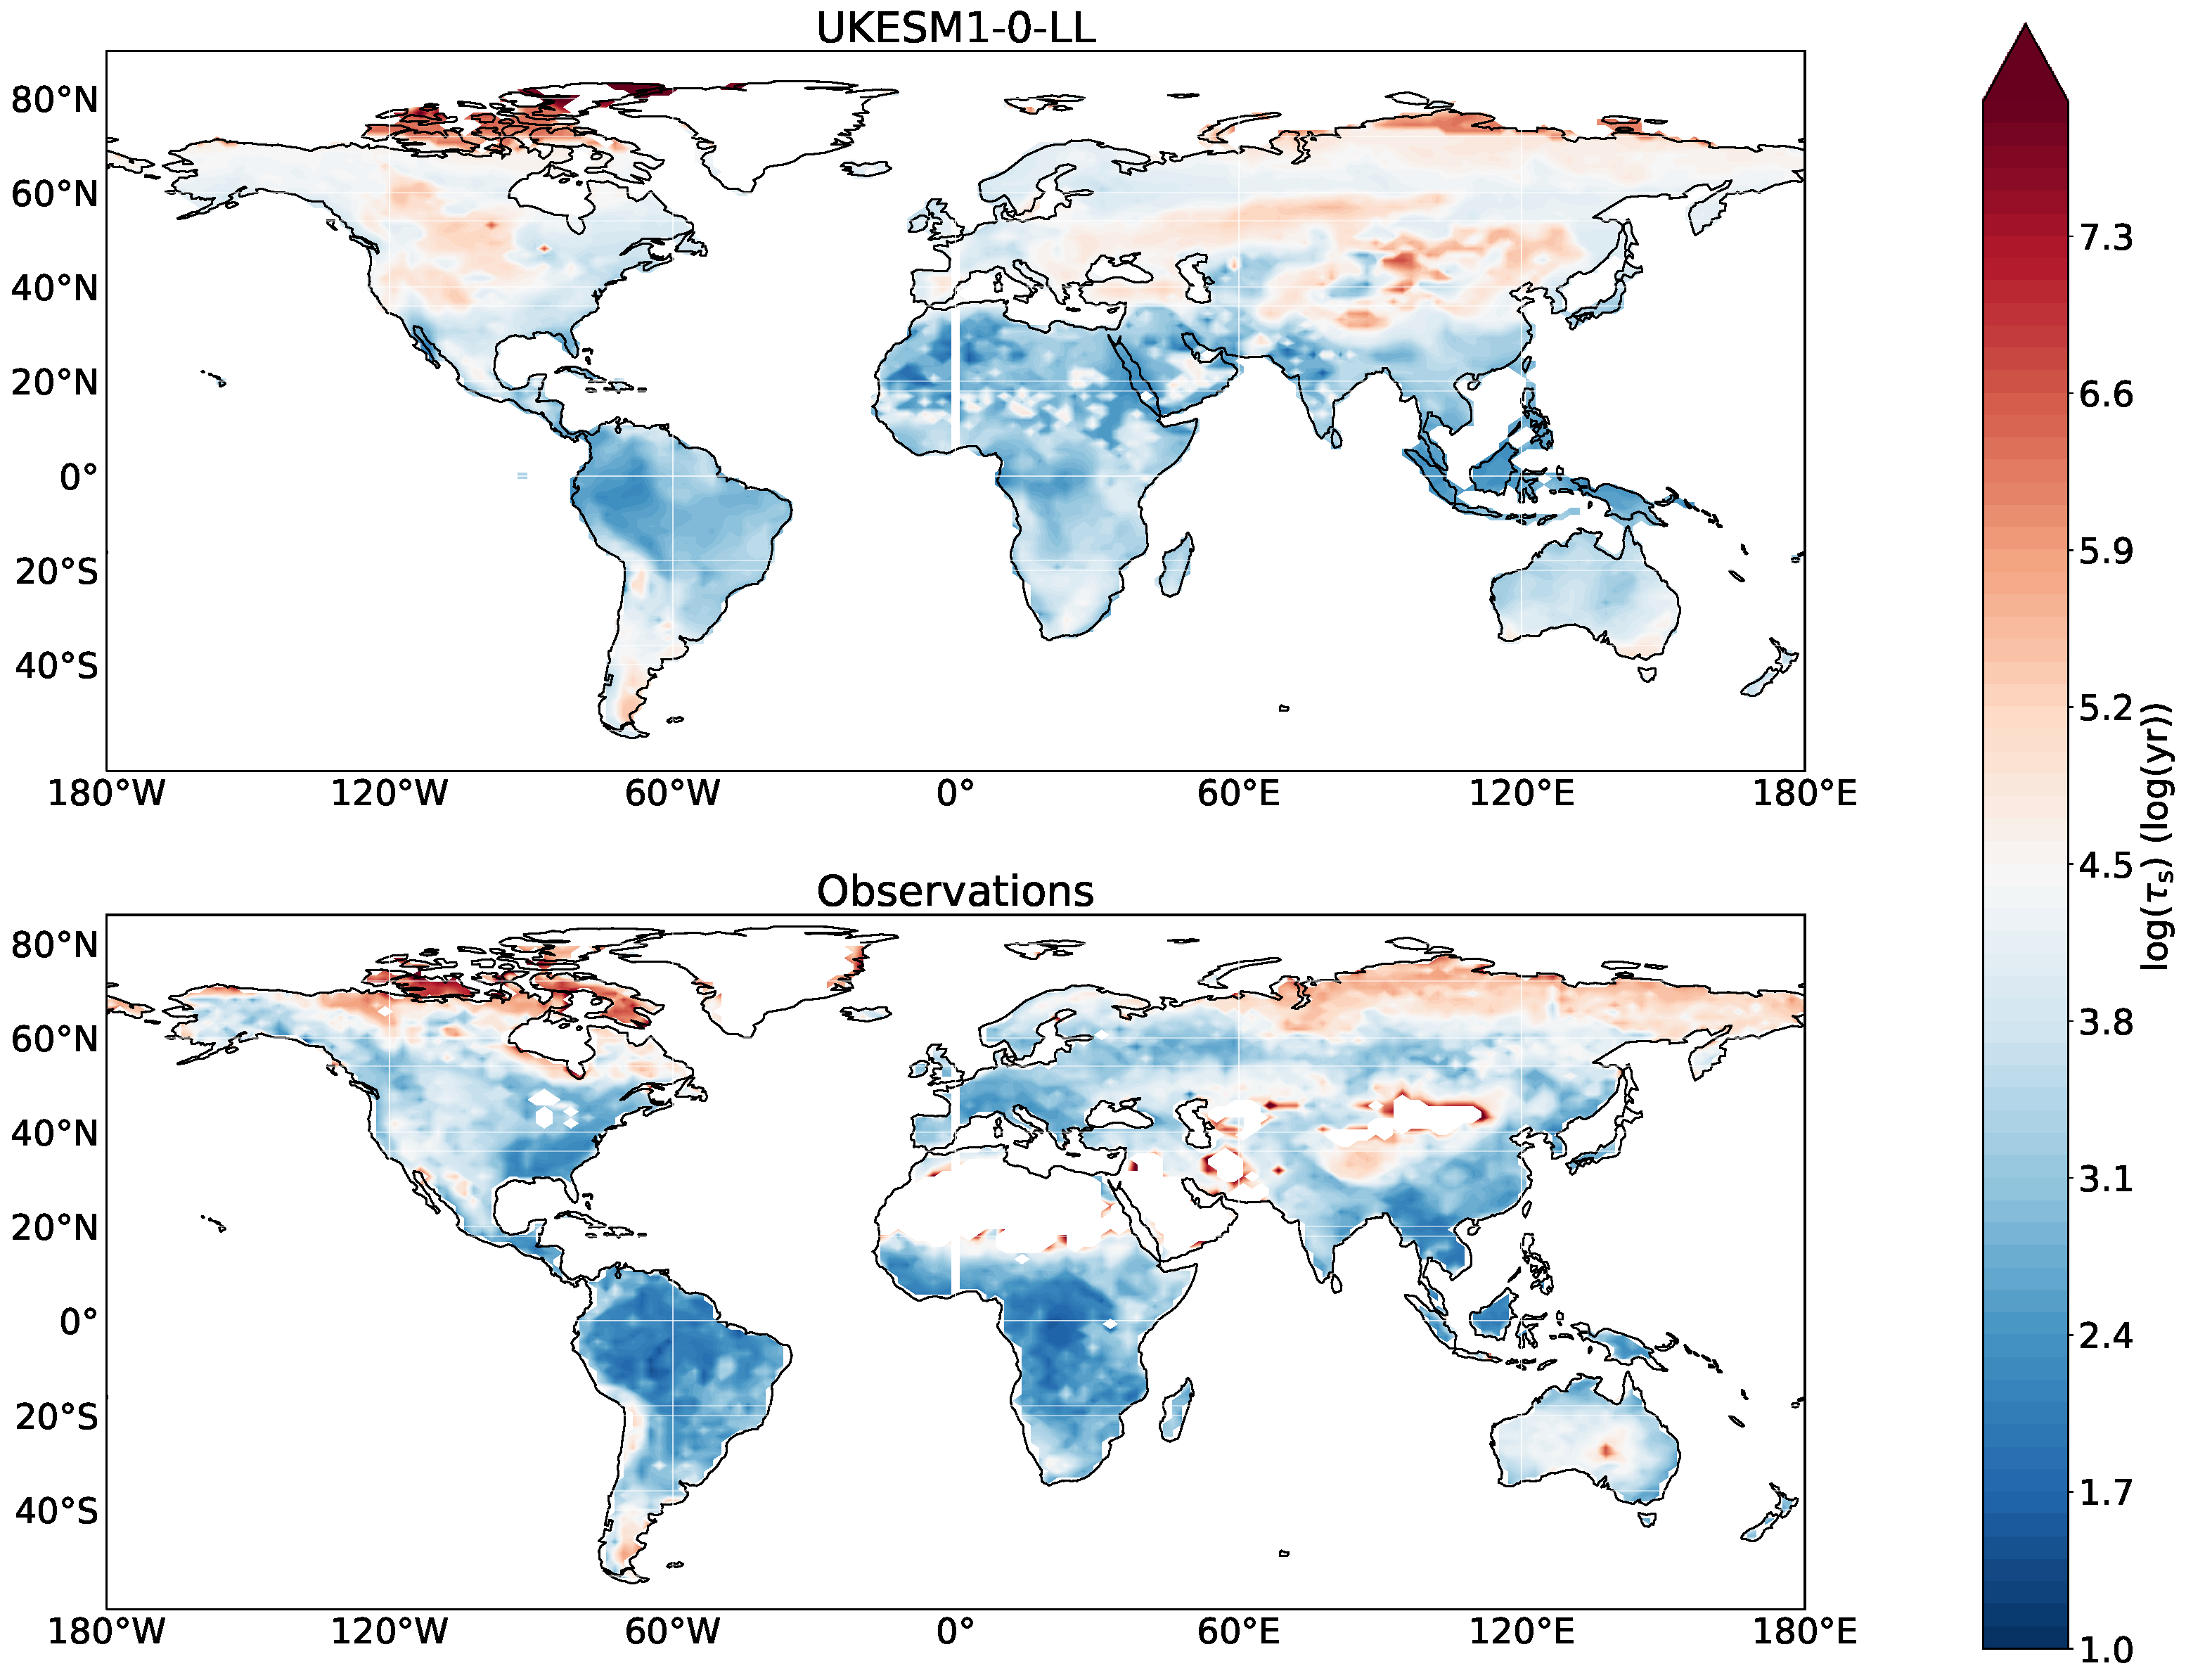
\includegraphics[width=12cm]{figs/Turnover/soil_tau_map_comparison.pdf}
    \caption{Soil turnover \label{fig:SoilTurnoverlMap}}
\end{figure*}

\begin{figure*}[t]
    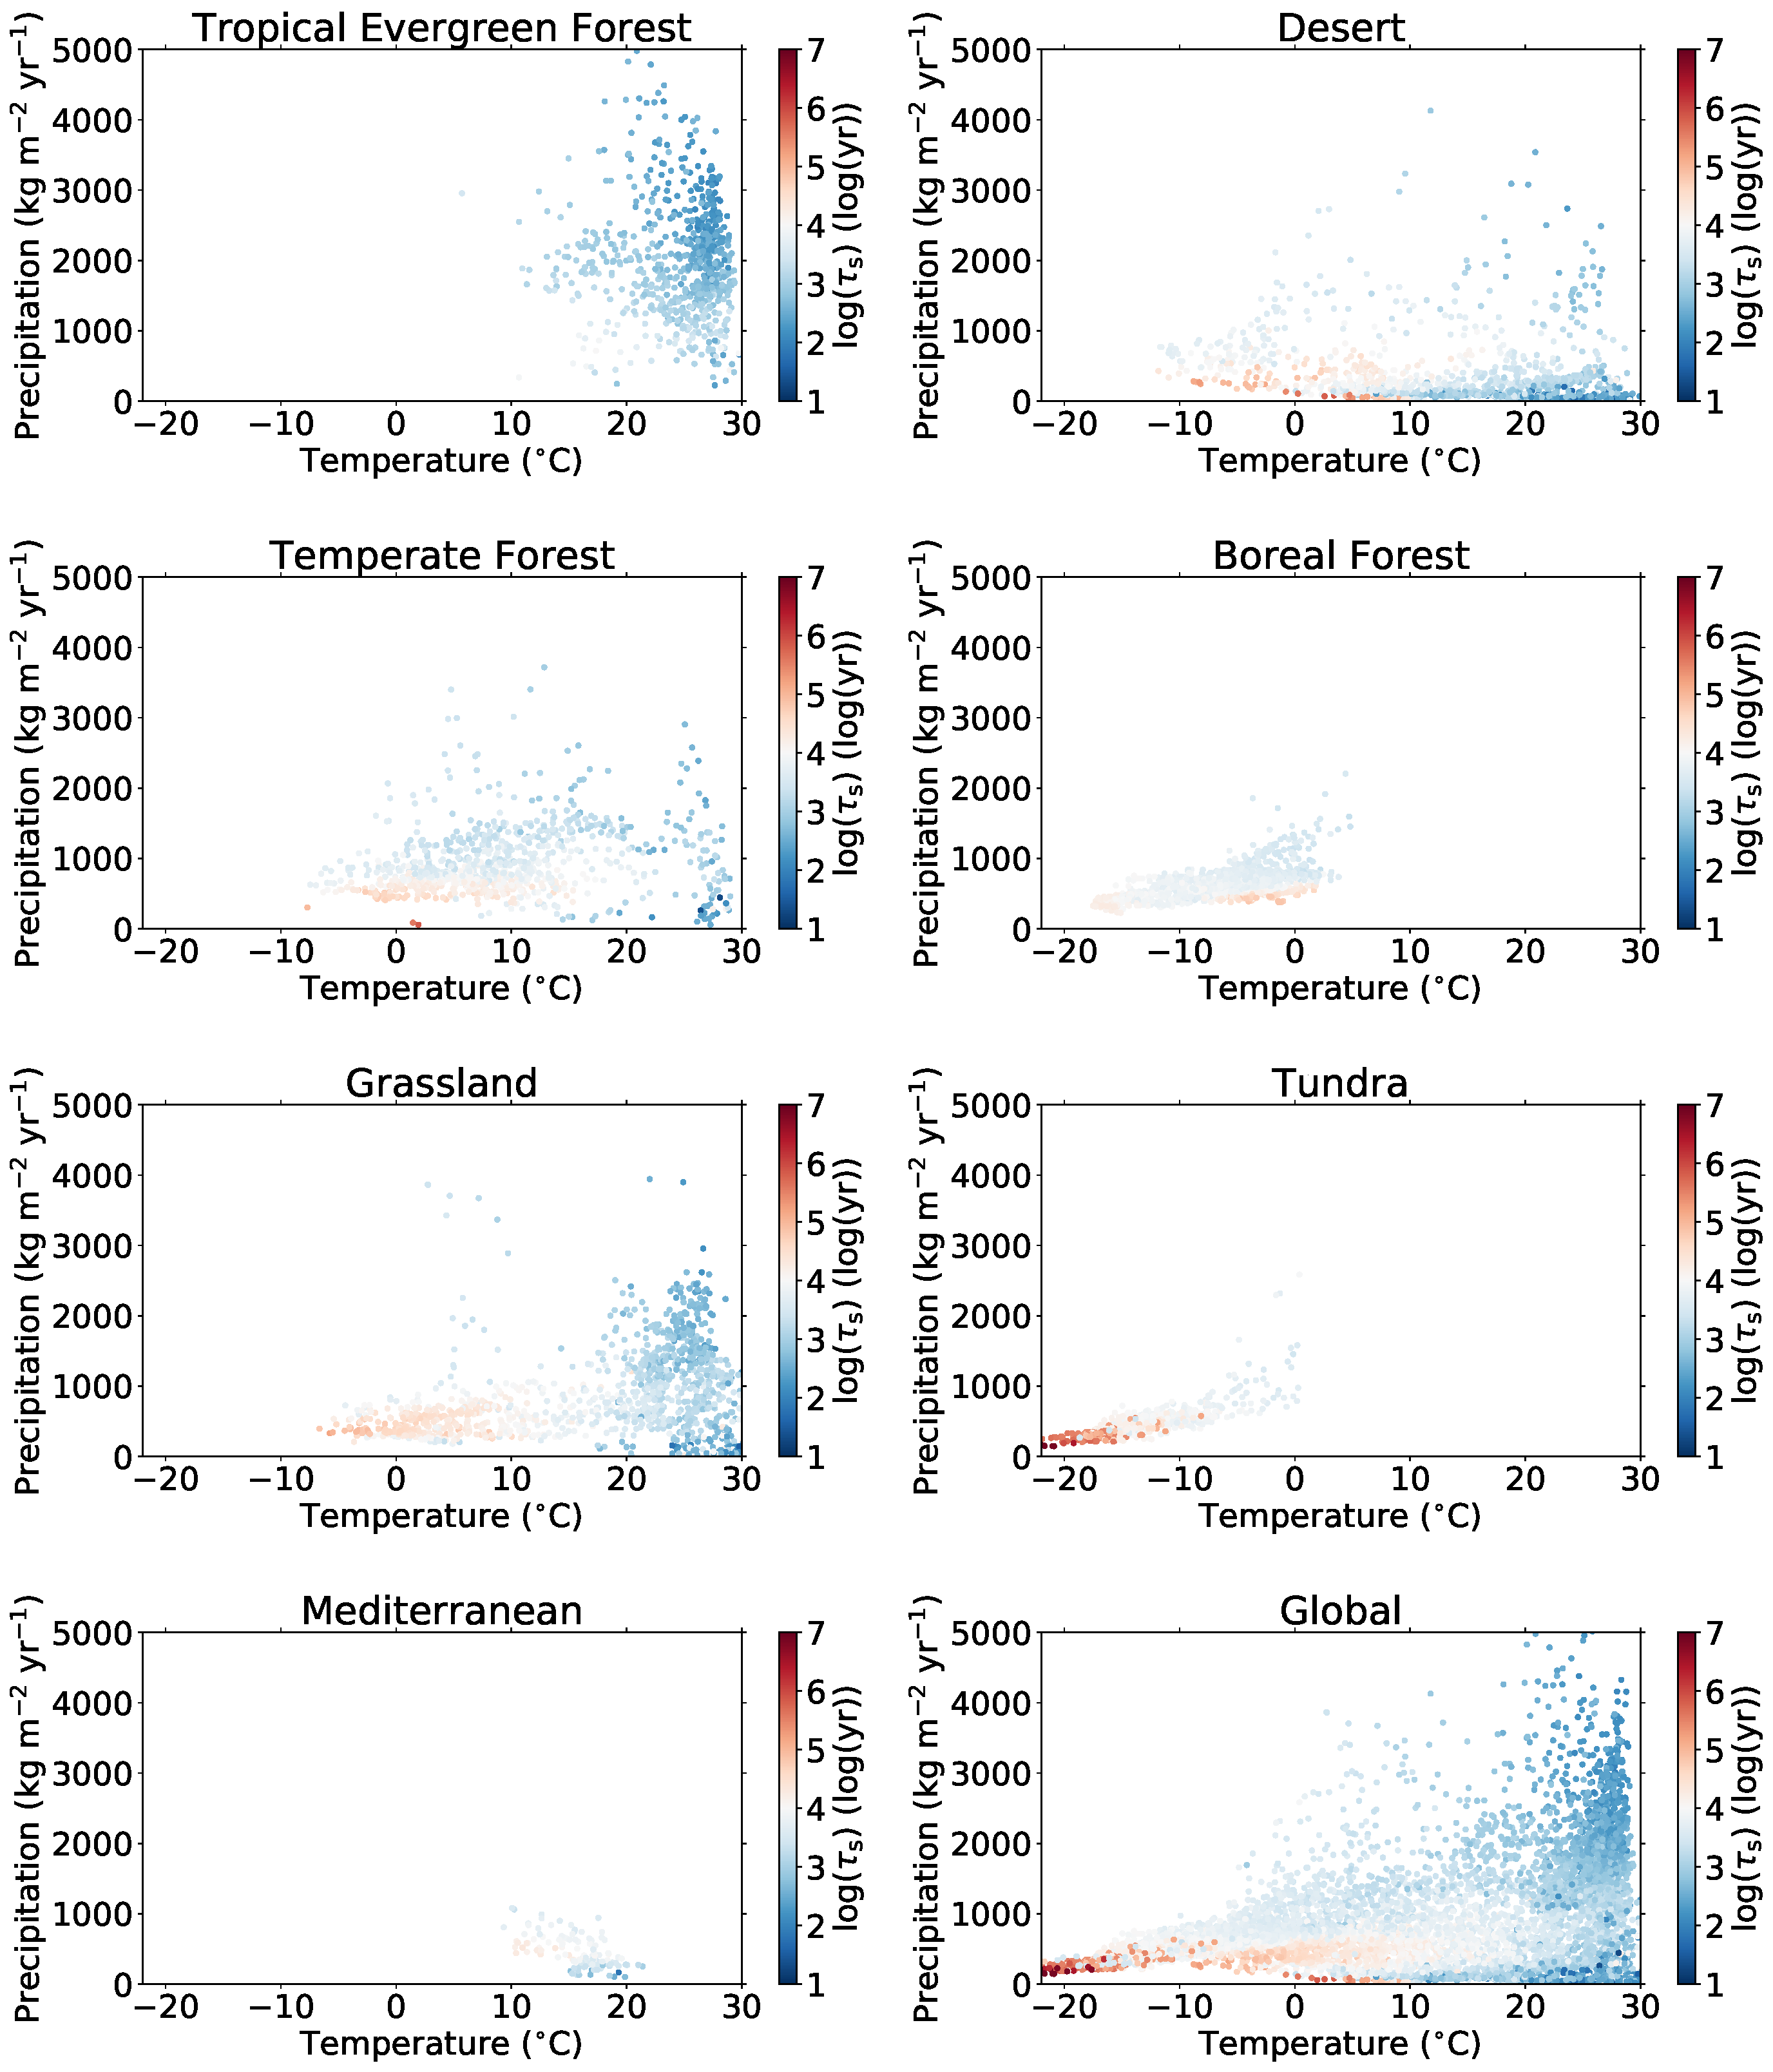
\includegraphics[width=6cm]{figs/Turnover/soil_UKESM_colouredbytau_biome_log.pdf}
    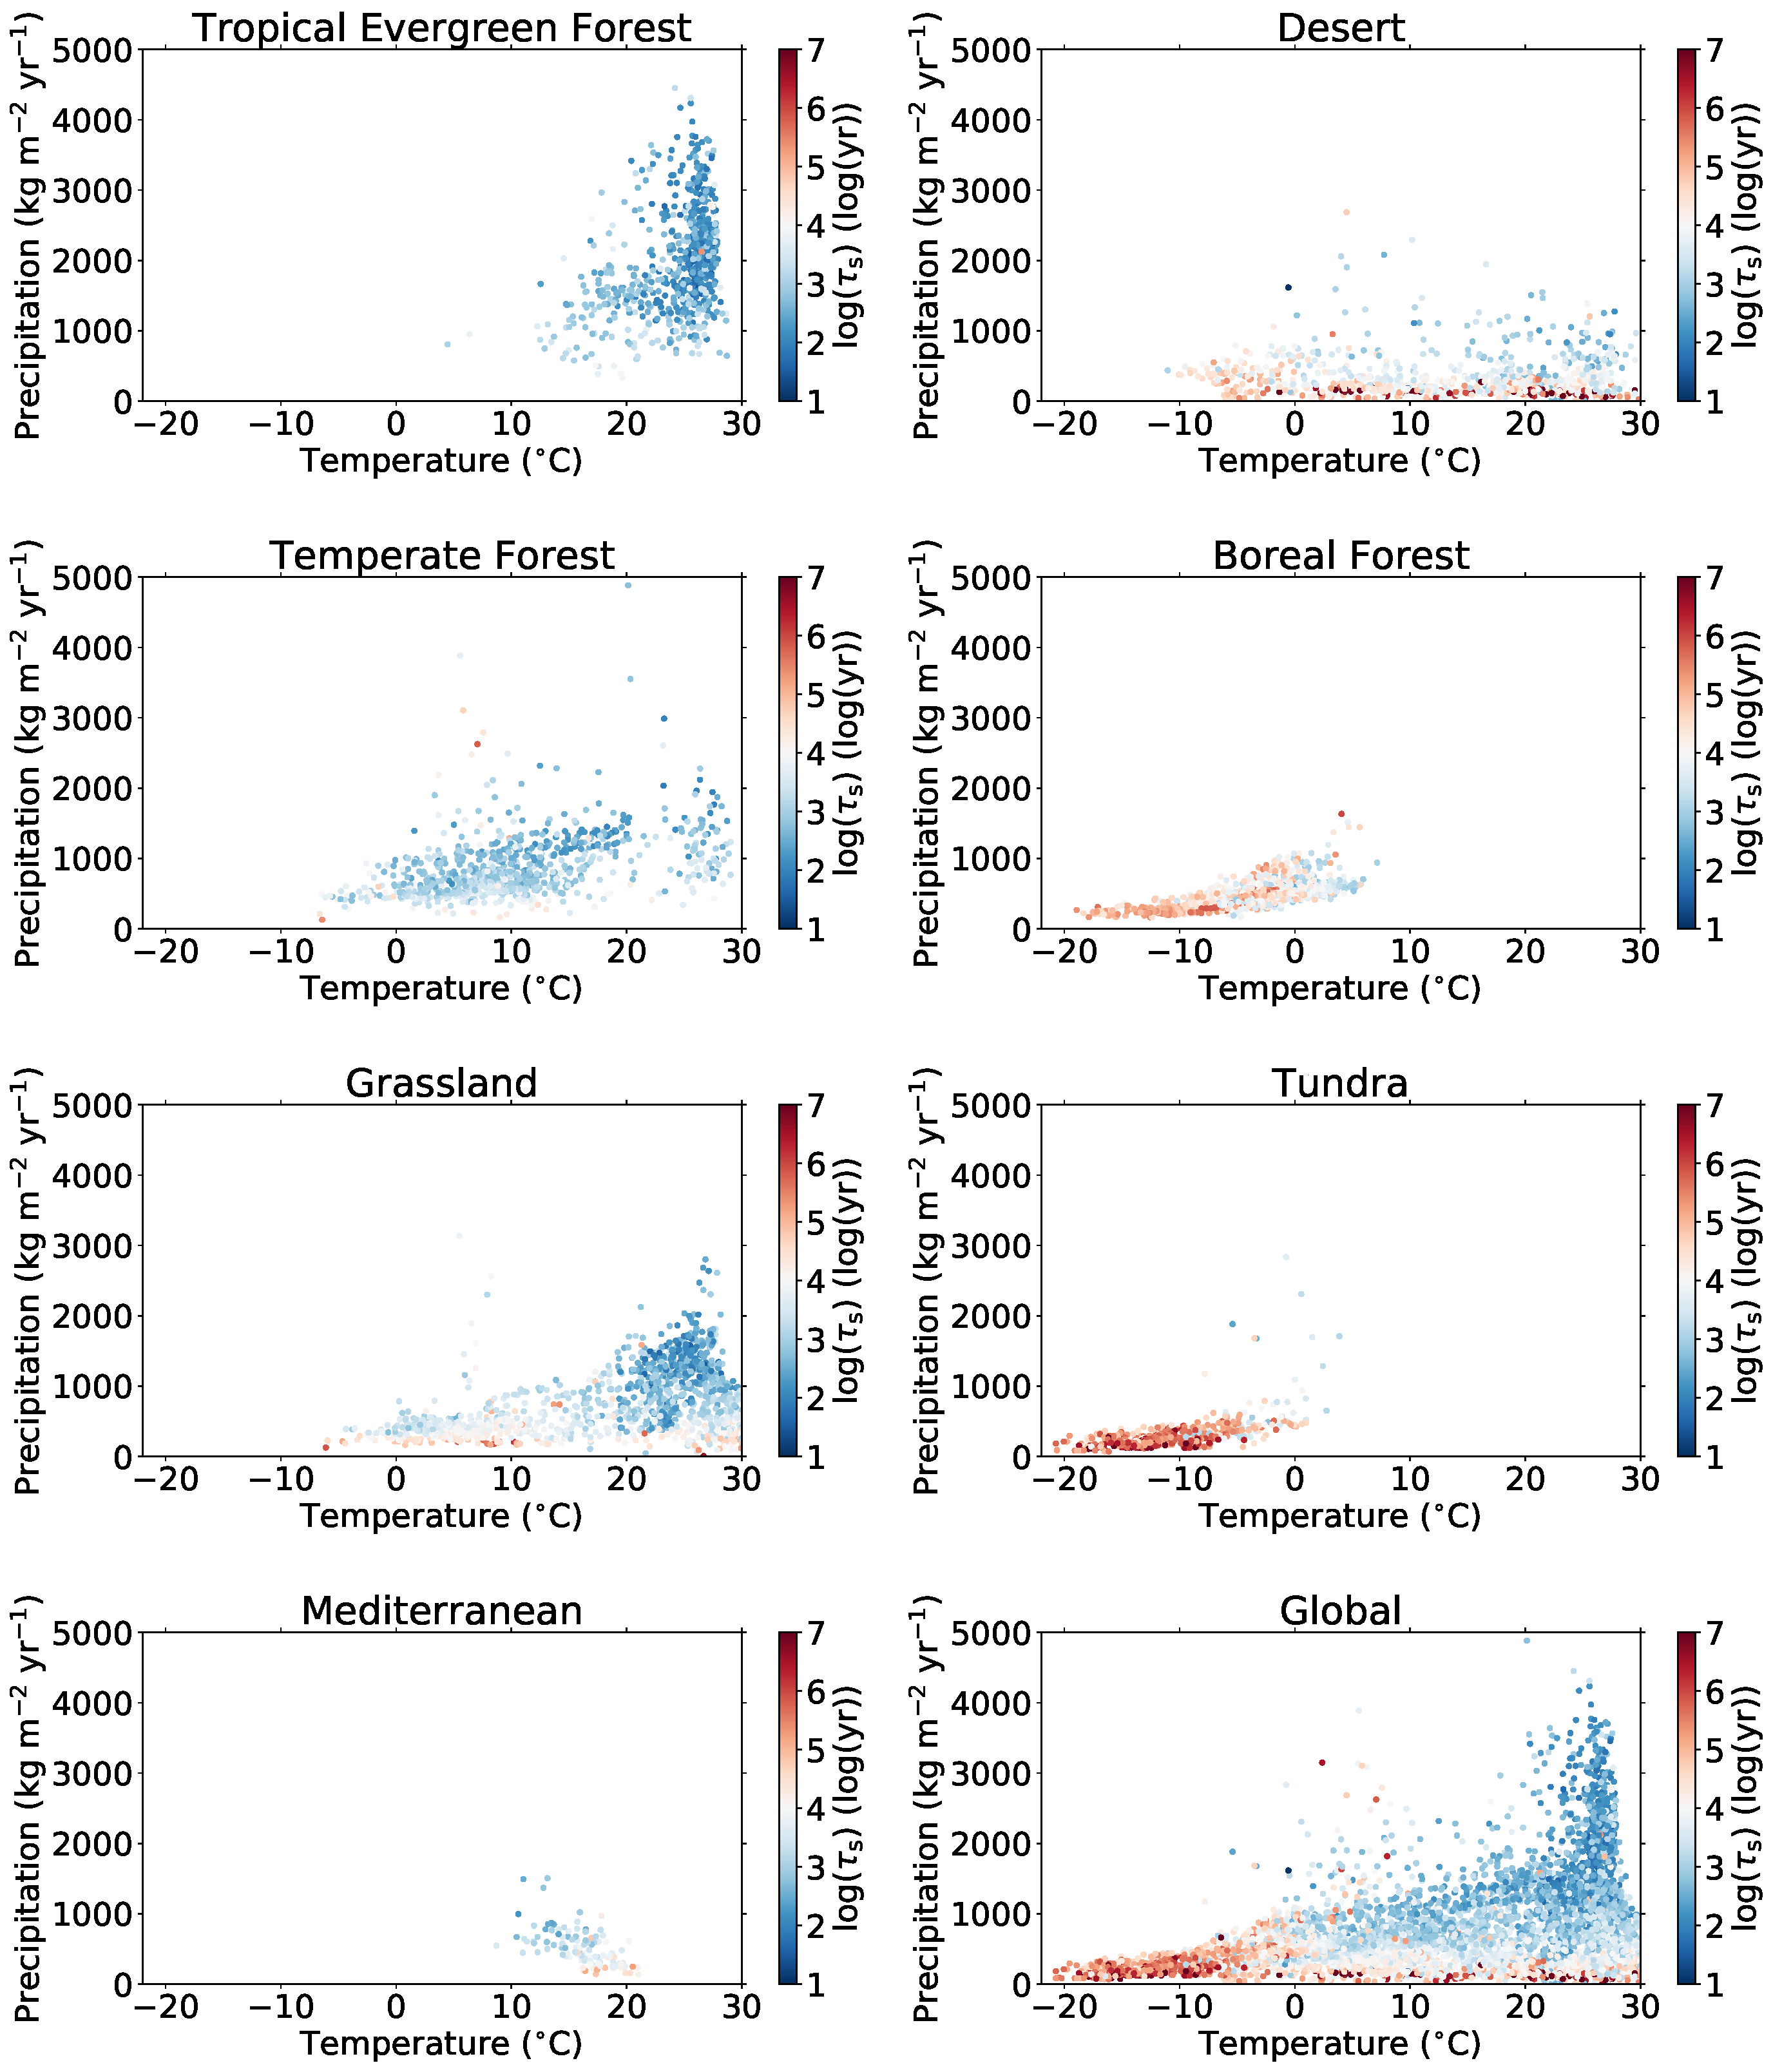
\includegraphics[width=6cm]{figs/Turnover/soil_obs1_colouredbytau_biome.pdf}
    \caption{Soil turnover \label{fig:EcoTurnoverlScatter}}
\end{figure*}

\hilight{Doug - add in SW maps}



\begin{figure*}[t]
    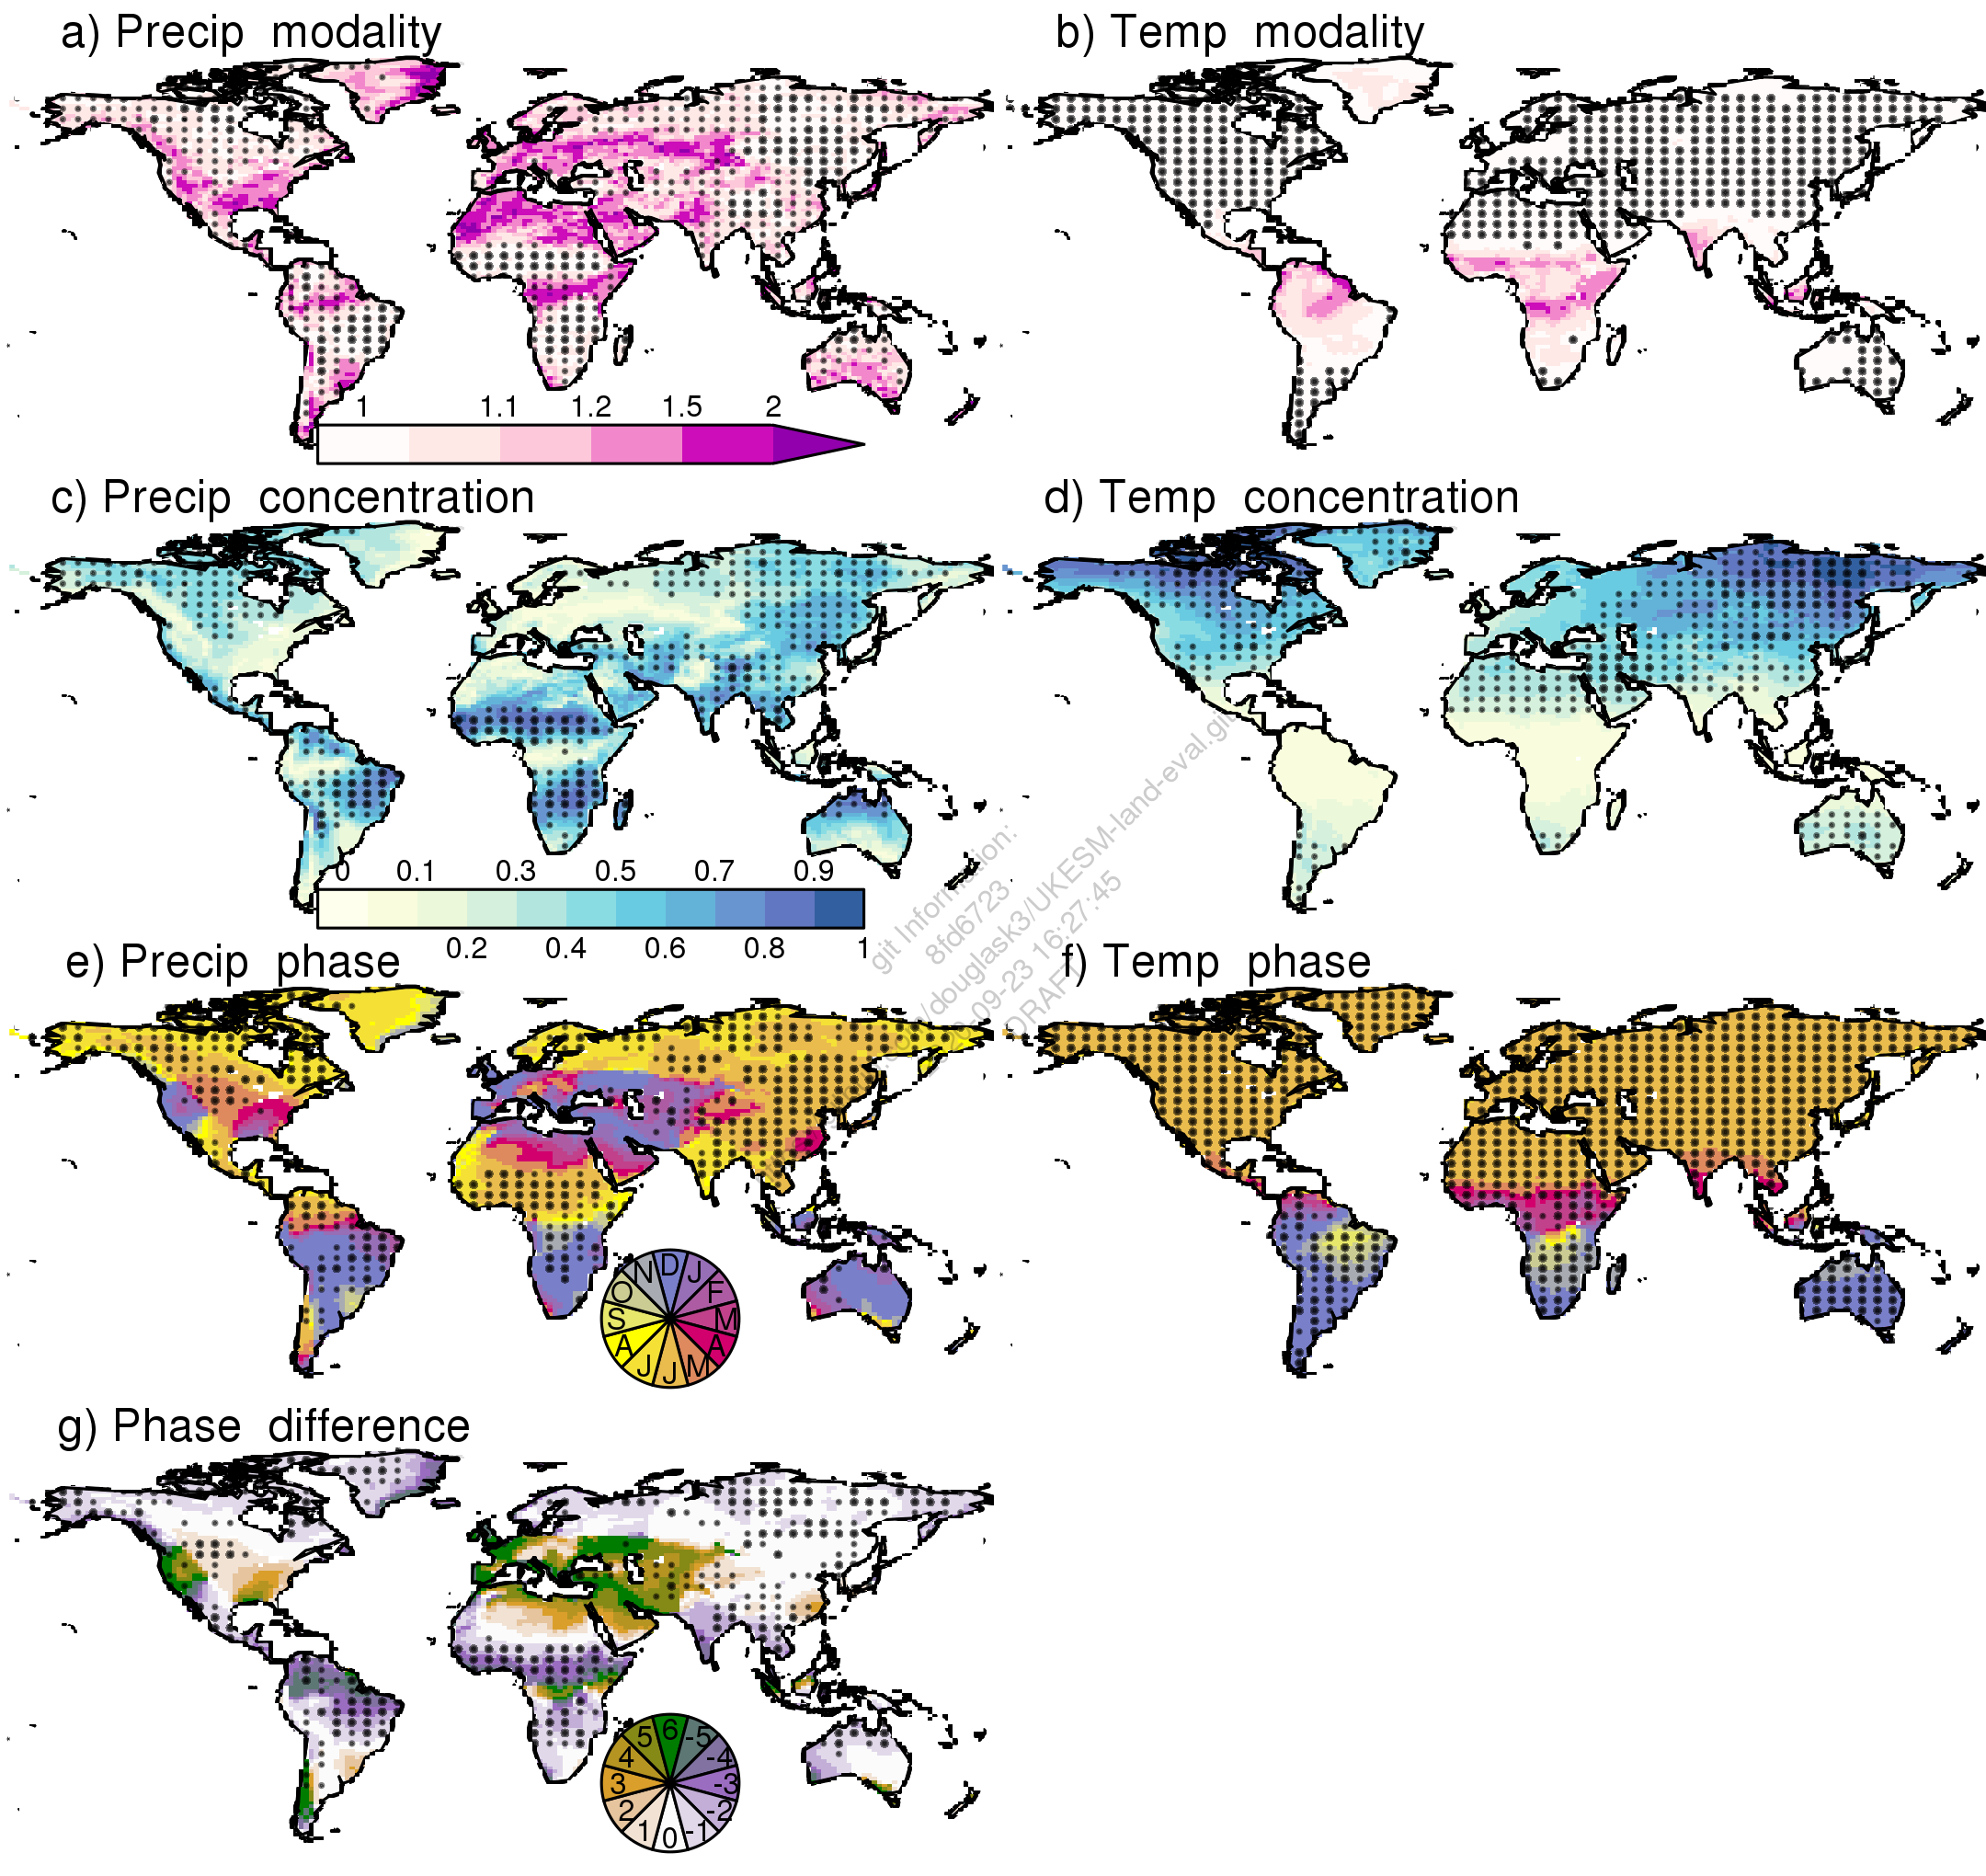
\includegraphics[width=12cm]{figs/Climate/climStuff-UKESM.png}
    \caption{UKESM precipitation (a, c, e) and temperature (b, d, f) seasonal metrics. a,b) modality; c,d) concentration; e,f) phase. g) shows the difference in phase between precip and temperature. Positive shows precip leading temperature, negative precip lagging temperature. Dots show smaller spread (higher confidence) across ensemble members. <<define>>  \label{fig:ClimateSeasonUKESMmaps}}
\end{figure*}

\begin{figure*}[t]
    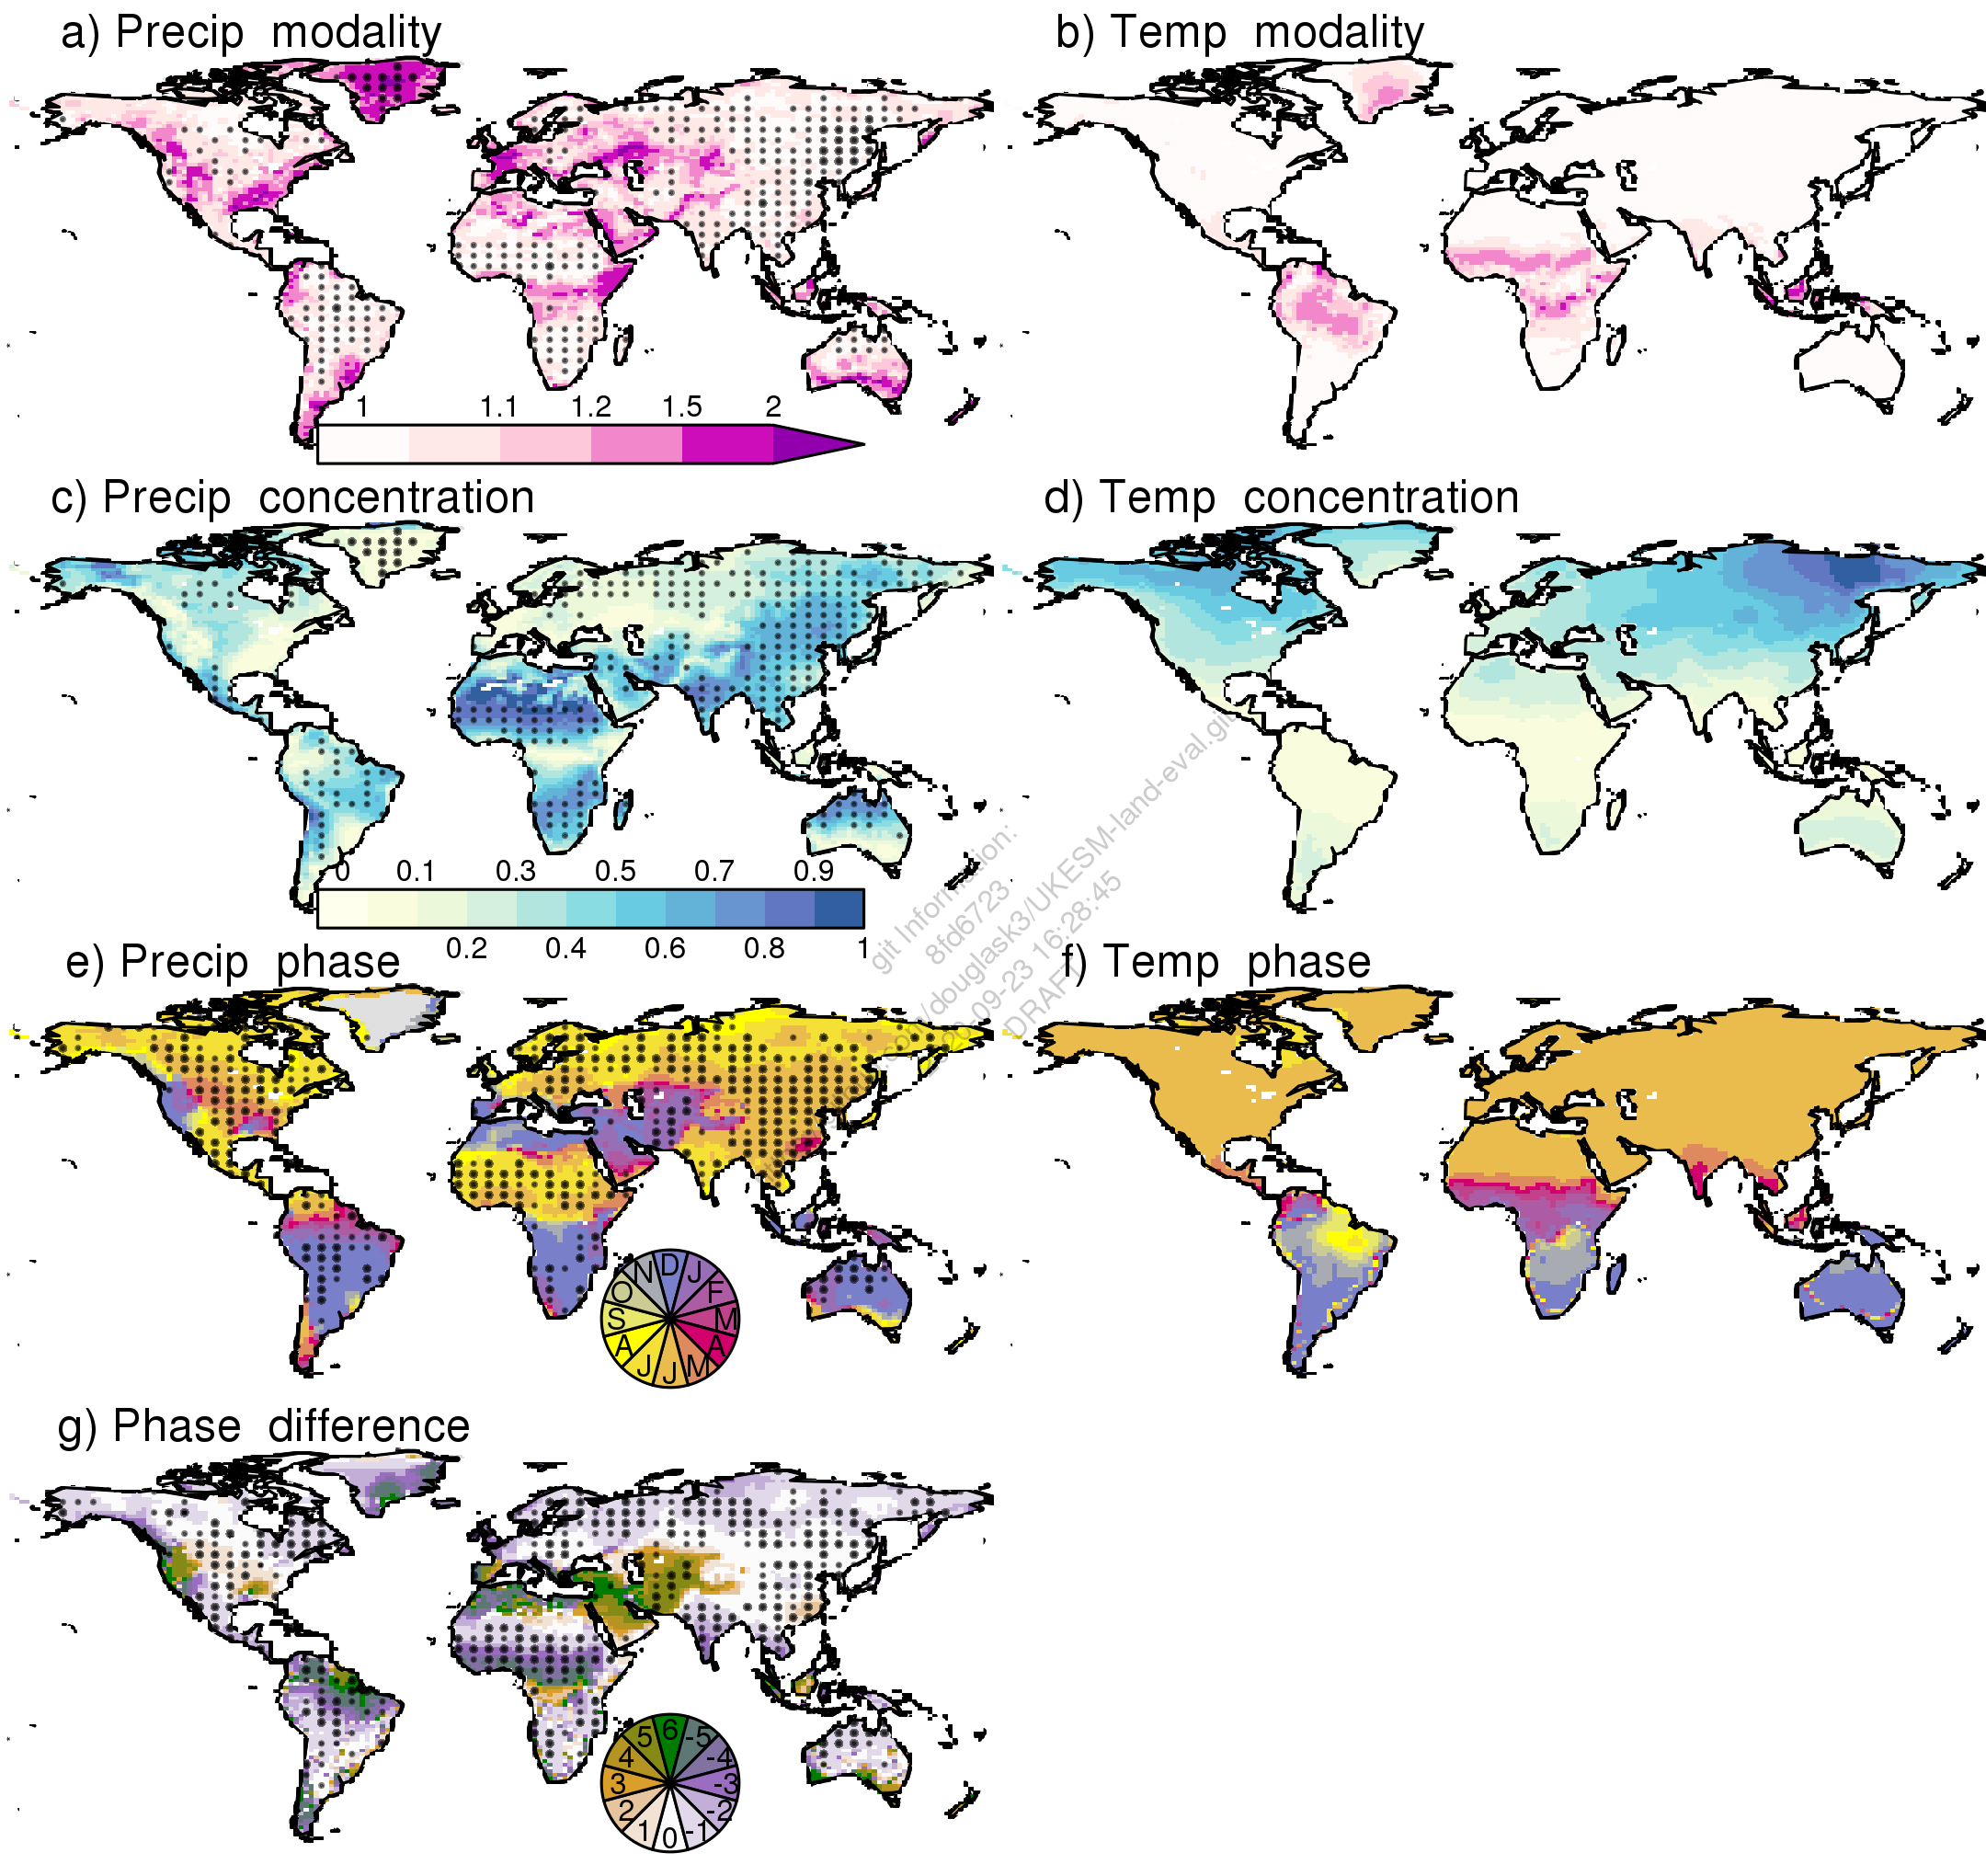
\includegraphics[width=12cm]{figs/Climate/climStuff-Observations.png}
    \caption{Observed precipitation (a, c, e) and temperature (b, d, f) seasonal metrics. a,b) modality; c,d) concentration; e,f) phase. g) shows the difference in phase between precip and temperature. Positive shows precip leading temperature, negative precip lagging temperature. Dots show smaller spread (higher confidence) across ensemble members. <<defibe>> \label{fig:ClimateSeasonObsMaps}}
\end{figure*}

\subsection{Drivers}
\hilight{Chantelle - Which figures to inlcude?}
\begin{figure*}[t]
    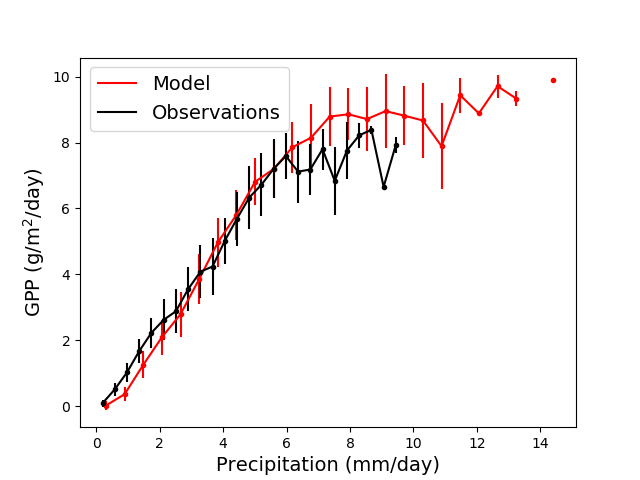
\includegraphics[width=6cm]{figs/GPPresponse/tl.png}
    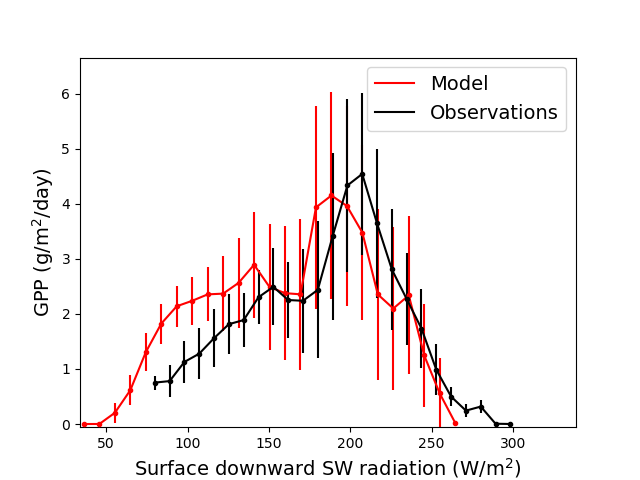
\includegraphics[width=6cm]{figs/GPPresponse/tr.png}
    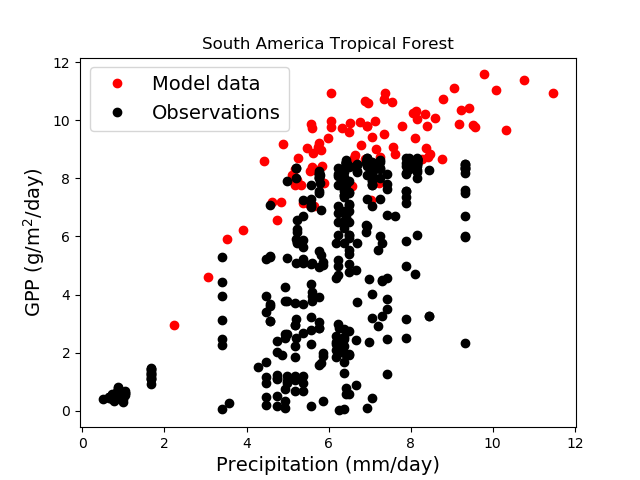
\includegraphics[width=6cm]{figs/GPPresponse/ml.png}
    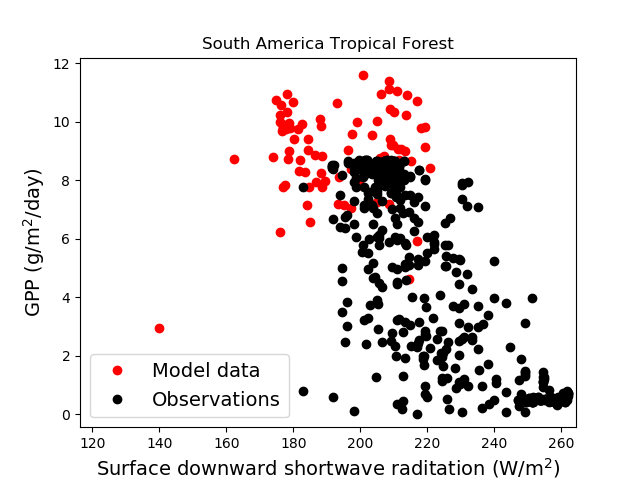
\includegraphics[width=6cm]{figs/GPPresponse/mr.png}
    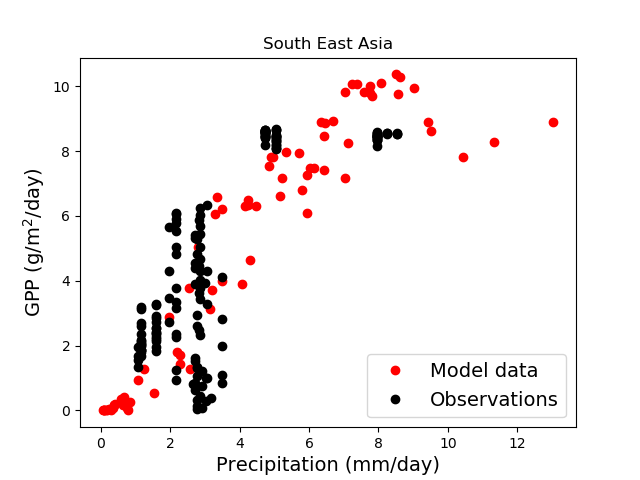
\includegraphics[width=6cm]{figs/GPPresponse/bl.png}
    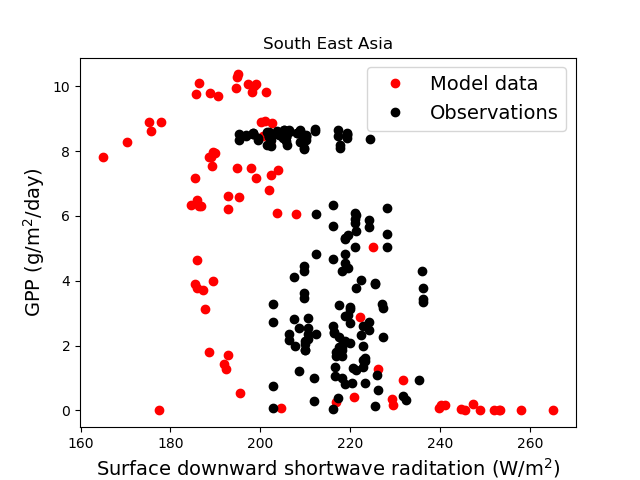
\includegraphics[width=6cm]{figs/GPPresponse/br.png}
    \caption{Response of GPP to precipitation (left column) and surface downward shortwave radiation (right column), for 1982-2008 ensemble mean. Top row shows global analysis, binned by independent variable (x). Data points show the mean, error bars show standard deviation range. Second and third rows show all data points for South America tropical forest, and South East Asia respectively. Observations are from GBAF (GPP), CERES (SWR), and GPCP2 (precipitation). \label{fig:GPPresponses}}
\end{figure*}

\hilight{Doug - add in new veg distribution scatter plots}

\begin{figure}[t]
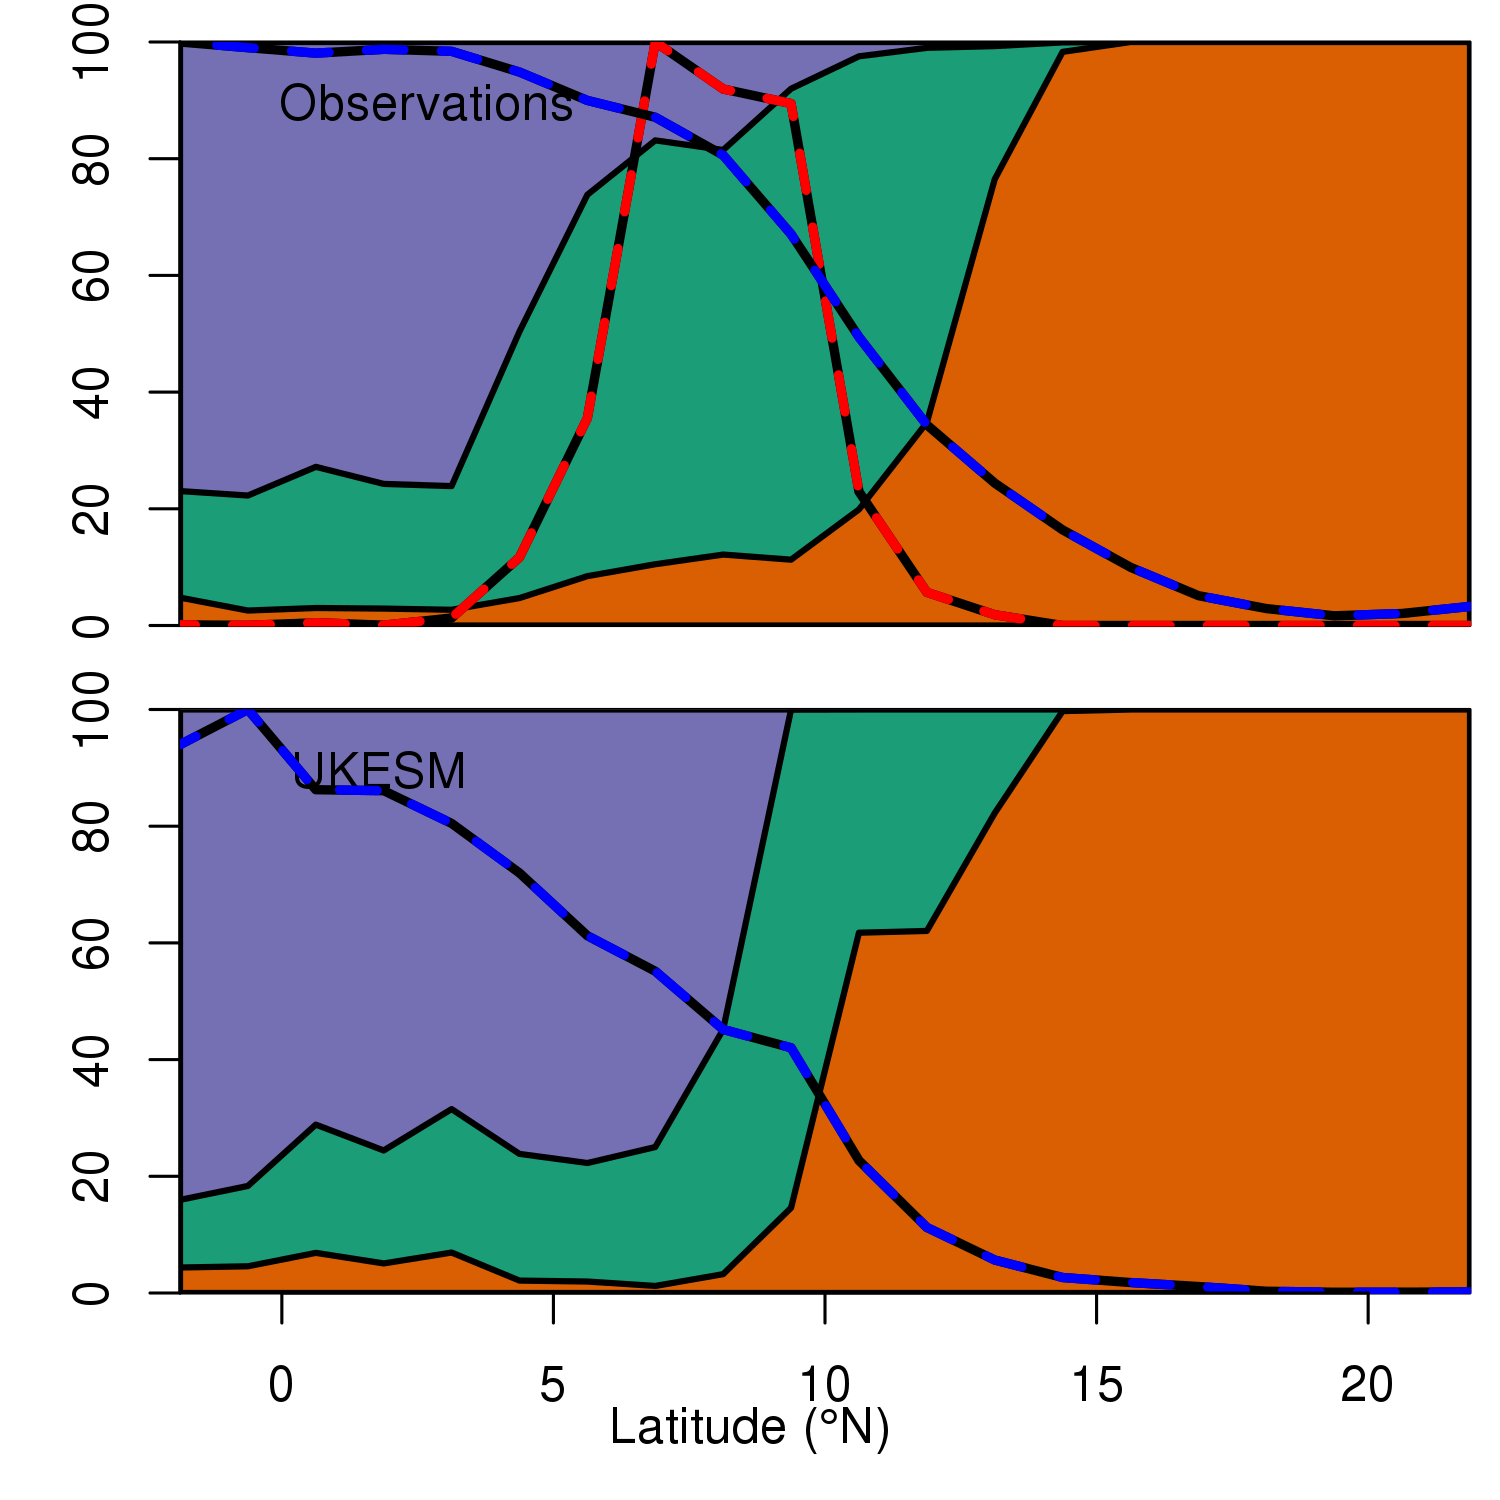
\includegraphics[width=8.3cm]{figs/trasect_AFRICA.png}
\caption{Transect of vegetation distribution from VCF observations and UKESM ensemble member u-bc179 along the longitude line of xx, spanning central Congo to central Sahara. Purple represents distribution of trees, green grasses and orange bare ground. Blue dotted line is observed mean annual precipitation from CRUTS 4.01 and u-bc179. Red dotted line is observed annual burnt area from GFED4s}
\end{figure}

\subsubsection{wetlands}
Generally good agreement is found between the two datasets, with large observed wetland fractions in the boreal regions reproduced in the model simulations. The tropical band of increased wetland fraction is found to be broader in the UKESM simulations than in the observations, particularly south of the Equator. We attribute much of this to a lack of tropical soils properties \citep{Gedney2019}.

Wetland methane emissions are primarily controlled by water table depth, temperature and available substrate. As such, adequately simulating the contemporary wetland area is important for modelling the methane cycle.  

\begin{figure*}[t]
    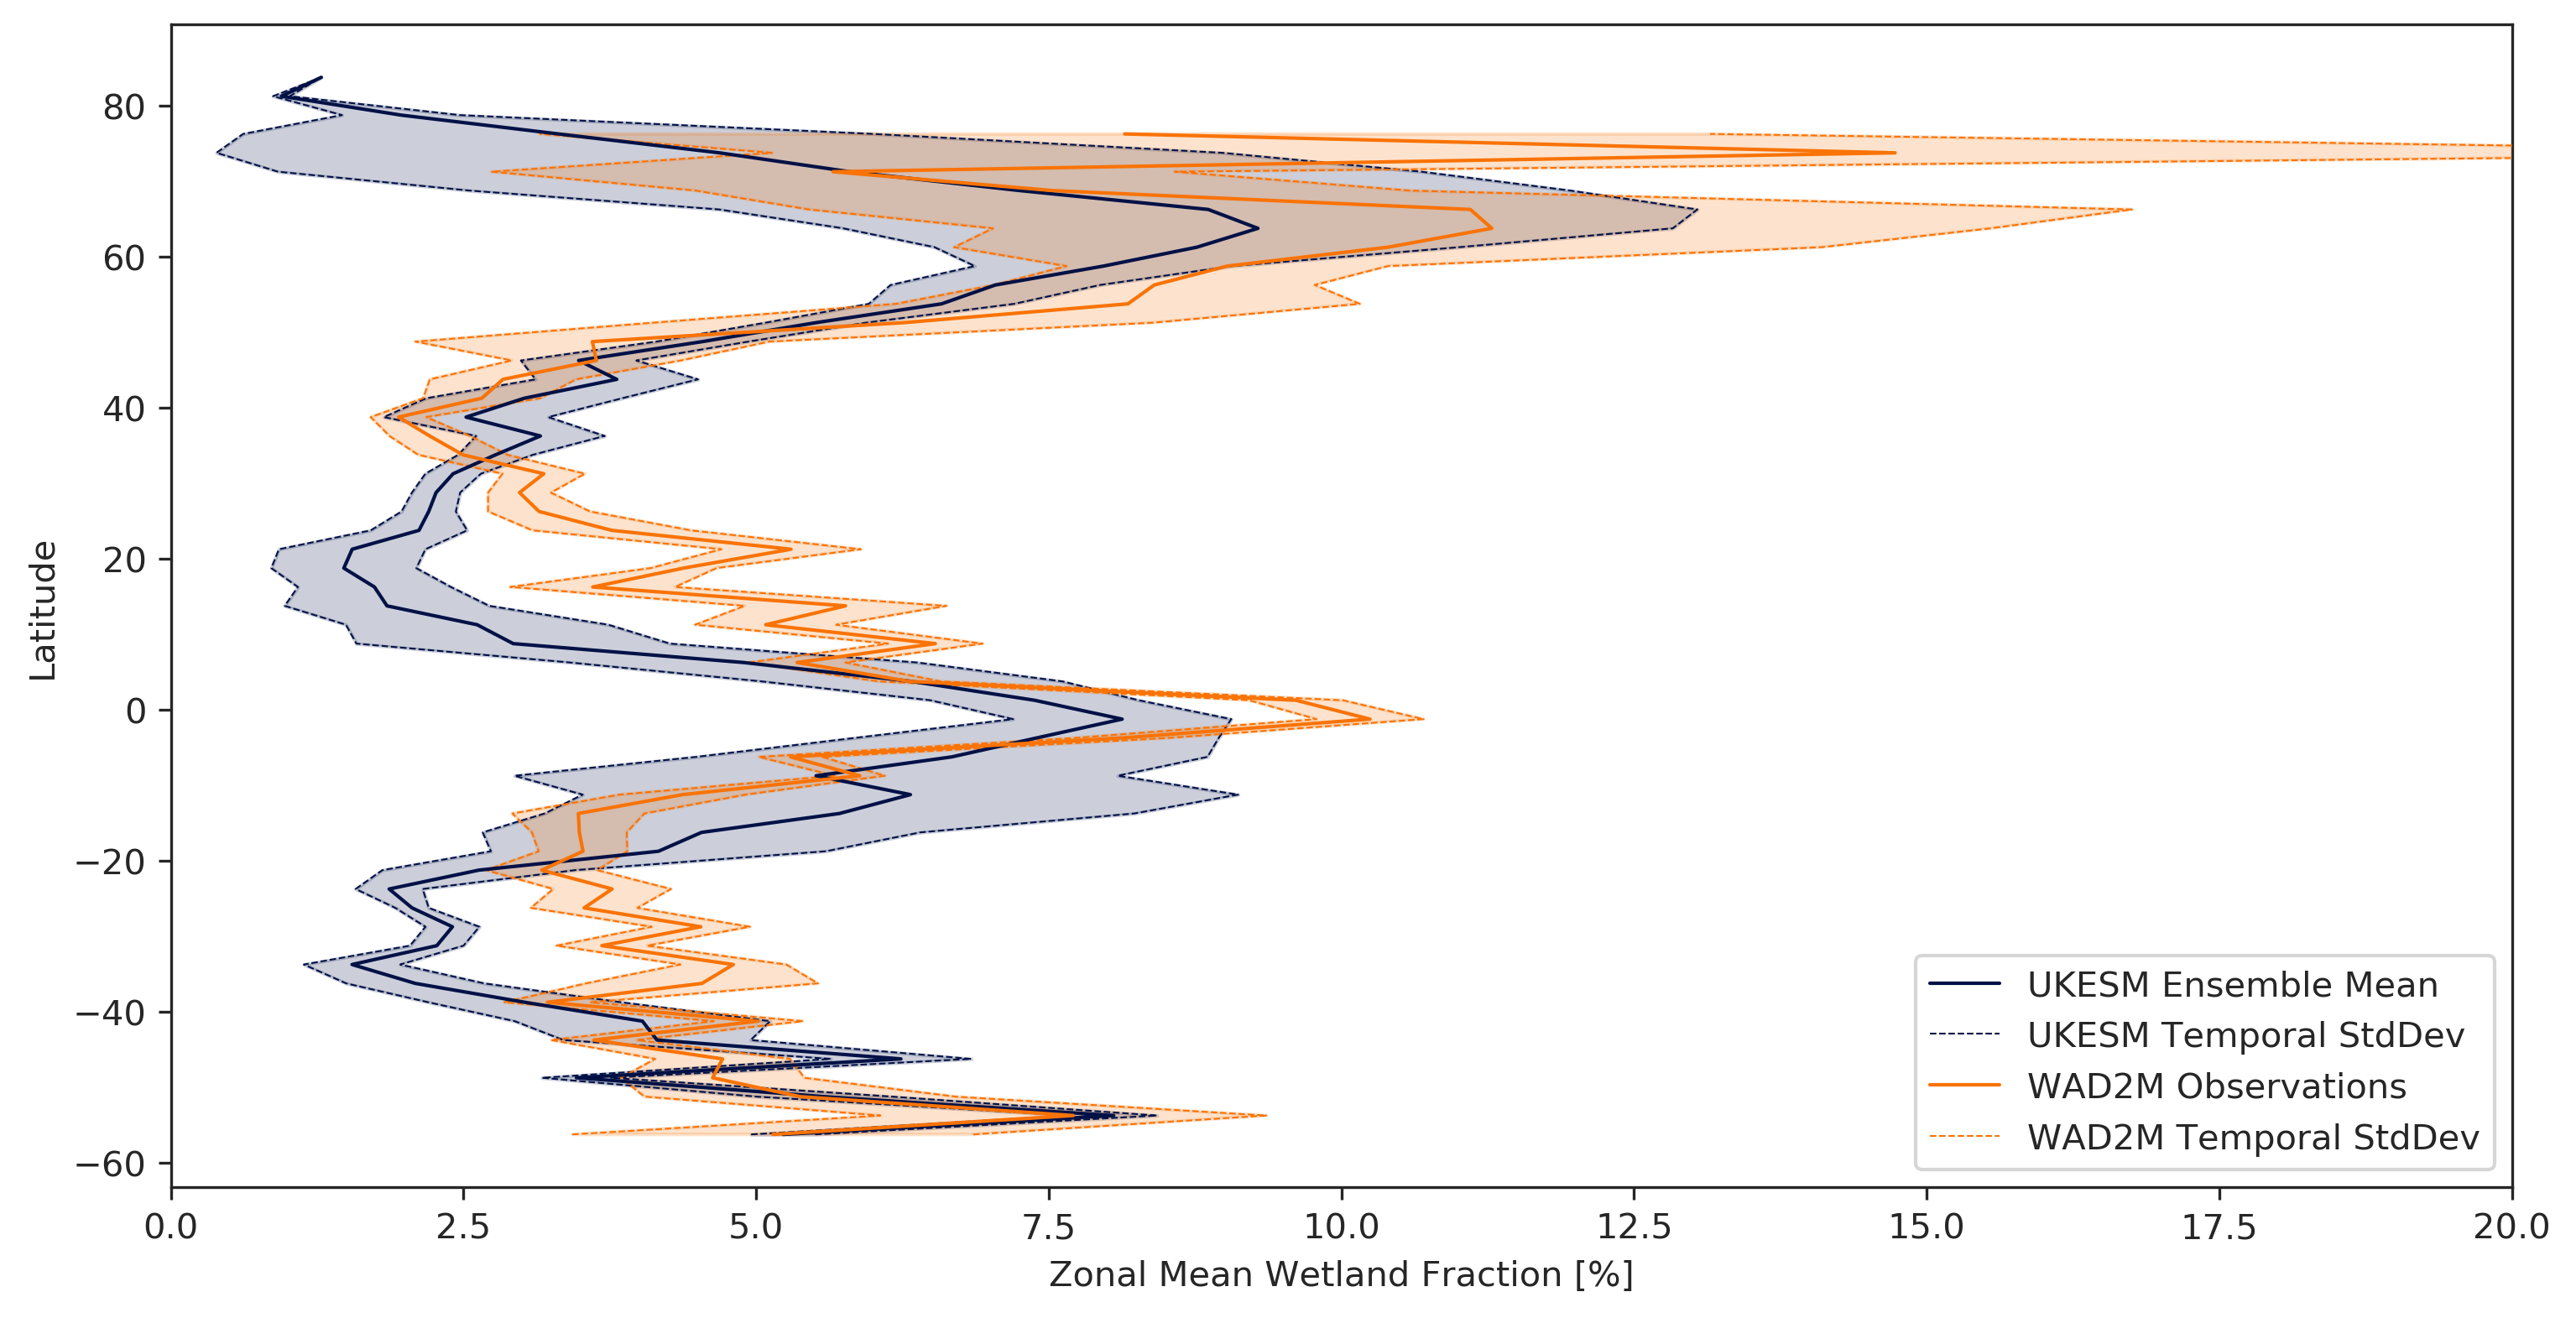
\includegraphics[width=16cm]{figs/Wetland.png}
    \caption{Zonal means in wetland extent for UKESM and observation.  \label{fig:wetland} }
\end{figure*}

\subsubsection{River flow}
There is a strong correlation with the multi-annual river flow (figure ***) \hilight{add figure} and obtain a correlation coefficient between modelled and observed for the multi-annual mean and log of river flow are 0.96 and 0.84 respectively. If we compare this to a similar off-line run where JULES is forced with observations we obtain correlation coefficients of 0.97 and 0.85 respectively, indicating that on a multi-year time scale UKESM is reproducing river flow well overall across the globe.

\section{Pathway for future development}

\subsection{Fire}
\hilight{Chantelle/Doug}
Within JULES, the land surface component of UKESM1, the INteractive Fire and Emission algoRithm for Natural envirOnments (INFERNO) is used to calculate burned area and fire emissions \citep{Mangeon2016}. Fuel and soil moisture simulated by the DGVM, together with climate reanalysis, gives flammability, which is combined with prescribed ignitions from population and lightning to diagnose burned area and species emissions. Recent developments to the model include coupling between burned area and dynamic vegetation to represent vegetation mortality, which improves the distribution of vegetation in offline simulations using climate reanalysis \citep{Burton2019}. Other work is ongoing in coupling fire emissions from INFERNO to the atmosphere-only configuration of UKESM1, enabling emissions and aerosols to influence atmospheric chemistry, radiation, clouds and weather and feedback on fire, as well as implementing lightening ignitions from the model \citep{Joao2020}. These component developments within the land-surface and atmosphere will be brought together to form a major new development of fully coupled fire in the next version of UKESM. 

\subsection{Soils}
\hilight{Eleanor(/Karina? - any summary from that specialy report thing?}  I've currently added the permafrost bit in the section below.....

\subsection{Permafrost}
Permafrost (soil which is permanently frozen) presence has been evaluated in both HadGEM3 and UKESM1 \citep{Sellar2019-bo,burke2020evaluating}. \cite{burke2020evaluating} found that the simulated permafrost extent fell within the range of the observations for both models. However, they also found that the maximum summer thaw depth was too deep. This is partly because the soil is poorly resolved with only 4 soil layers in the top 3 m. Therefore one priority for the next configuration is to increase the number of soil layers. Recent developments in an offline version of JULES include a vertically resolved soil biogeochemsitry model \citep{wiltshire2020jules,burke2017vertical}. This enables the permafrost carbon feedback to be quantified \citep{burke2017quantifying} and will be included in a future version of UKESM.

\subsection{Inundation}
Inundation in UKESM is currently limited to that caused by groundwater. Incorporating inundation caused by rivers "over-banking" in JULES is currently underway  \citep{Dadson2010,Lewis2018} and is a priority for the next configuration. The large amount of evaporation from inundated open water is also important and should be included \citep{Dadson2010}. Adding tropical soils are shown to improve the spatial pattern of inundation in the tropics \citep{Gedney2019}.


\subsection{Methane}
\hilight{Gerd agreed to provide paragraph}

add some stuff about soil moisture

\conclusions  %% \conclusions[modified heading if necessary]
TEXT

%% The following commands are for the statements about the availability of data sets and/or software code corresponding to the manuscript.
%% It is strongly recommended to make use of these sections in case data sets and/or software code have been part of your research the article is based on.

\codeavailability{TEXT} %% use this section when having only software code available


\dataavailability{TEXT} %% use this section when having only data sets available


\codedataavailability{TEXT} %% use this section when having data sets and software code available


%\sampleavailability{TEXT} %% use this section when having geoscientific samples available


\videosupplement{TEXT} %% use this section when having video supplements available


\appendix
\section{}    %% Appendix A

\subsection{}     %% Appendix A1, A2, etc.


\noappendix       %% use this to mark the end of the appendix section

%% Regarding figures and tables in appendices, the following two options are possible depending on your general handling of figures and tables in the manuscript environment:

%% Option 1: If you sorted all figures and tables into the sections of the text, please also sort the appendix figures and appendix tables into the respective appendix sections.
%% They will be correctly named automatically.

%% Option 2: If you put all figures after the reference list, please insert appendix tables and figures after the normal tables and figures.
%% To rename them correctly to A1, A2, etc., please add the following commands in front of them:

\appendixfigures  %% needs to be added in front of appendix figures
\begin{figure}[t]
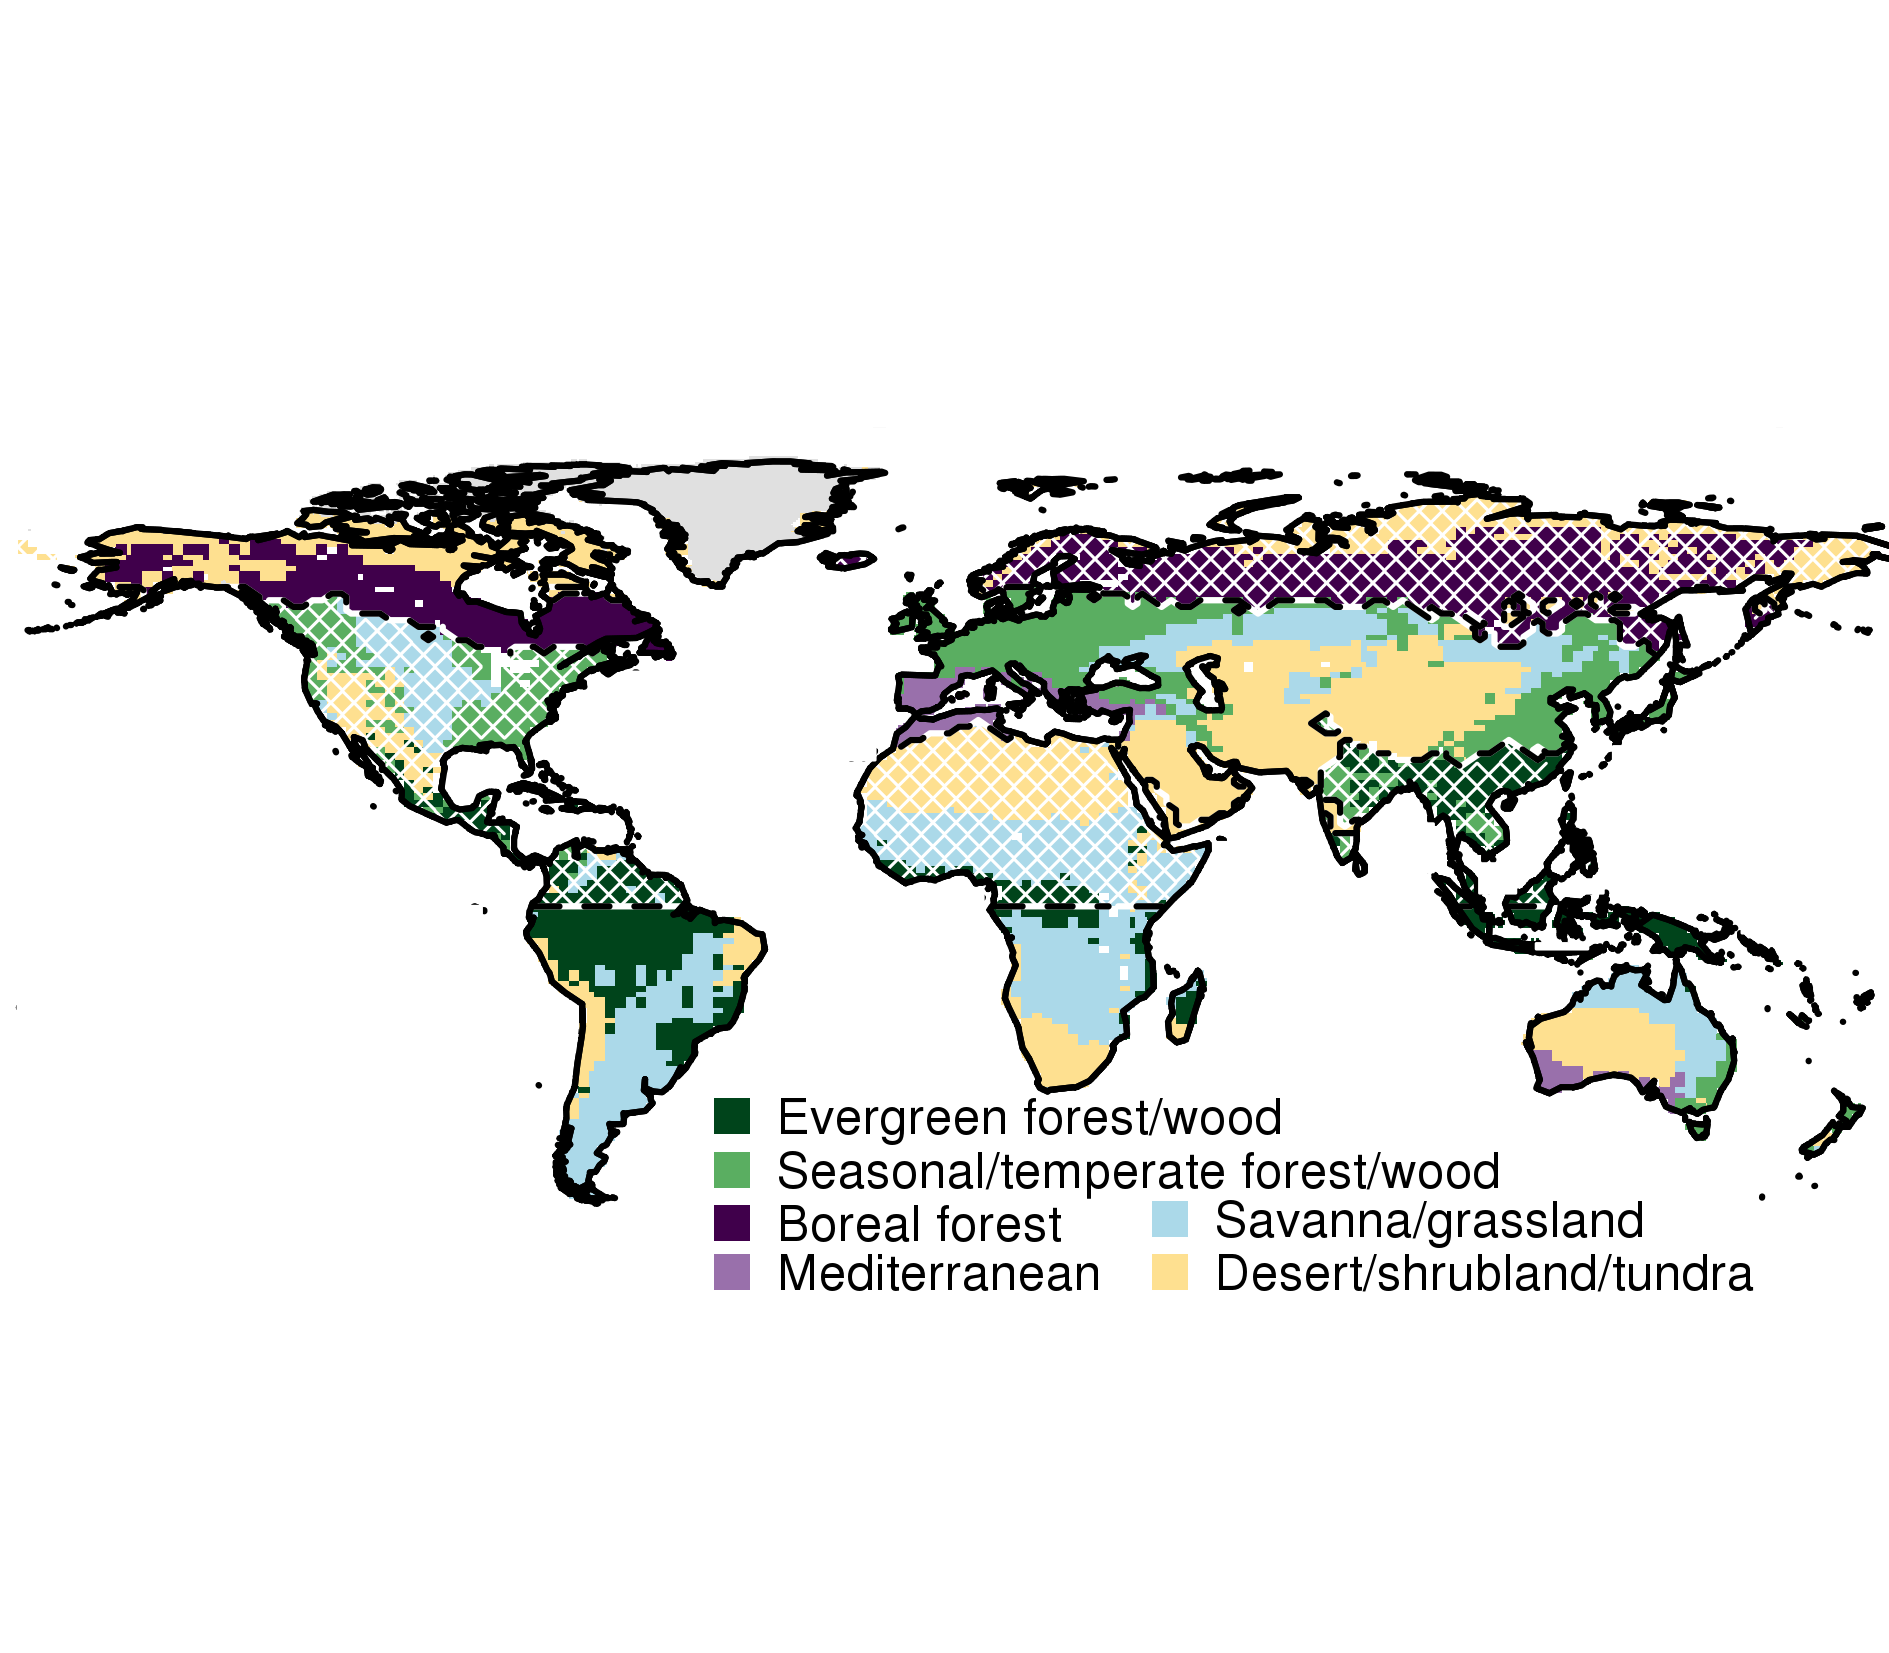
\includegraphics[width=8.3cm]{figs/biomeMap.png}
\caption{Biomes/realms used in this study, based on \citet{Olson2001-gv}, as per \citet{Sellar2019-bo}. Grouping of the ecosystems in\citet{Olson2001-gv} into biomes is similar to \citet{Kelley2019-yu} and realms follow \citet{Olson2001-gv} with Americas and Africa split into Northern and Southern (Tables A1-3).
 \label{fig:regionsMap}}
\end{figure}

\begin{figure}[t]
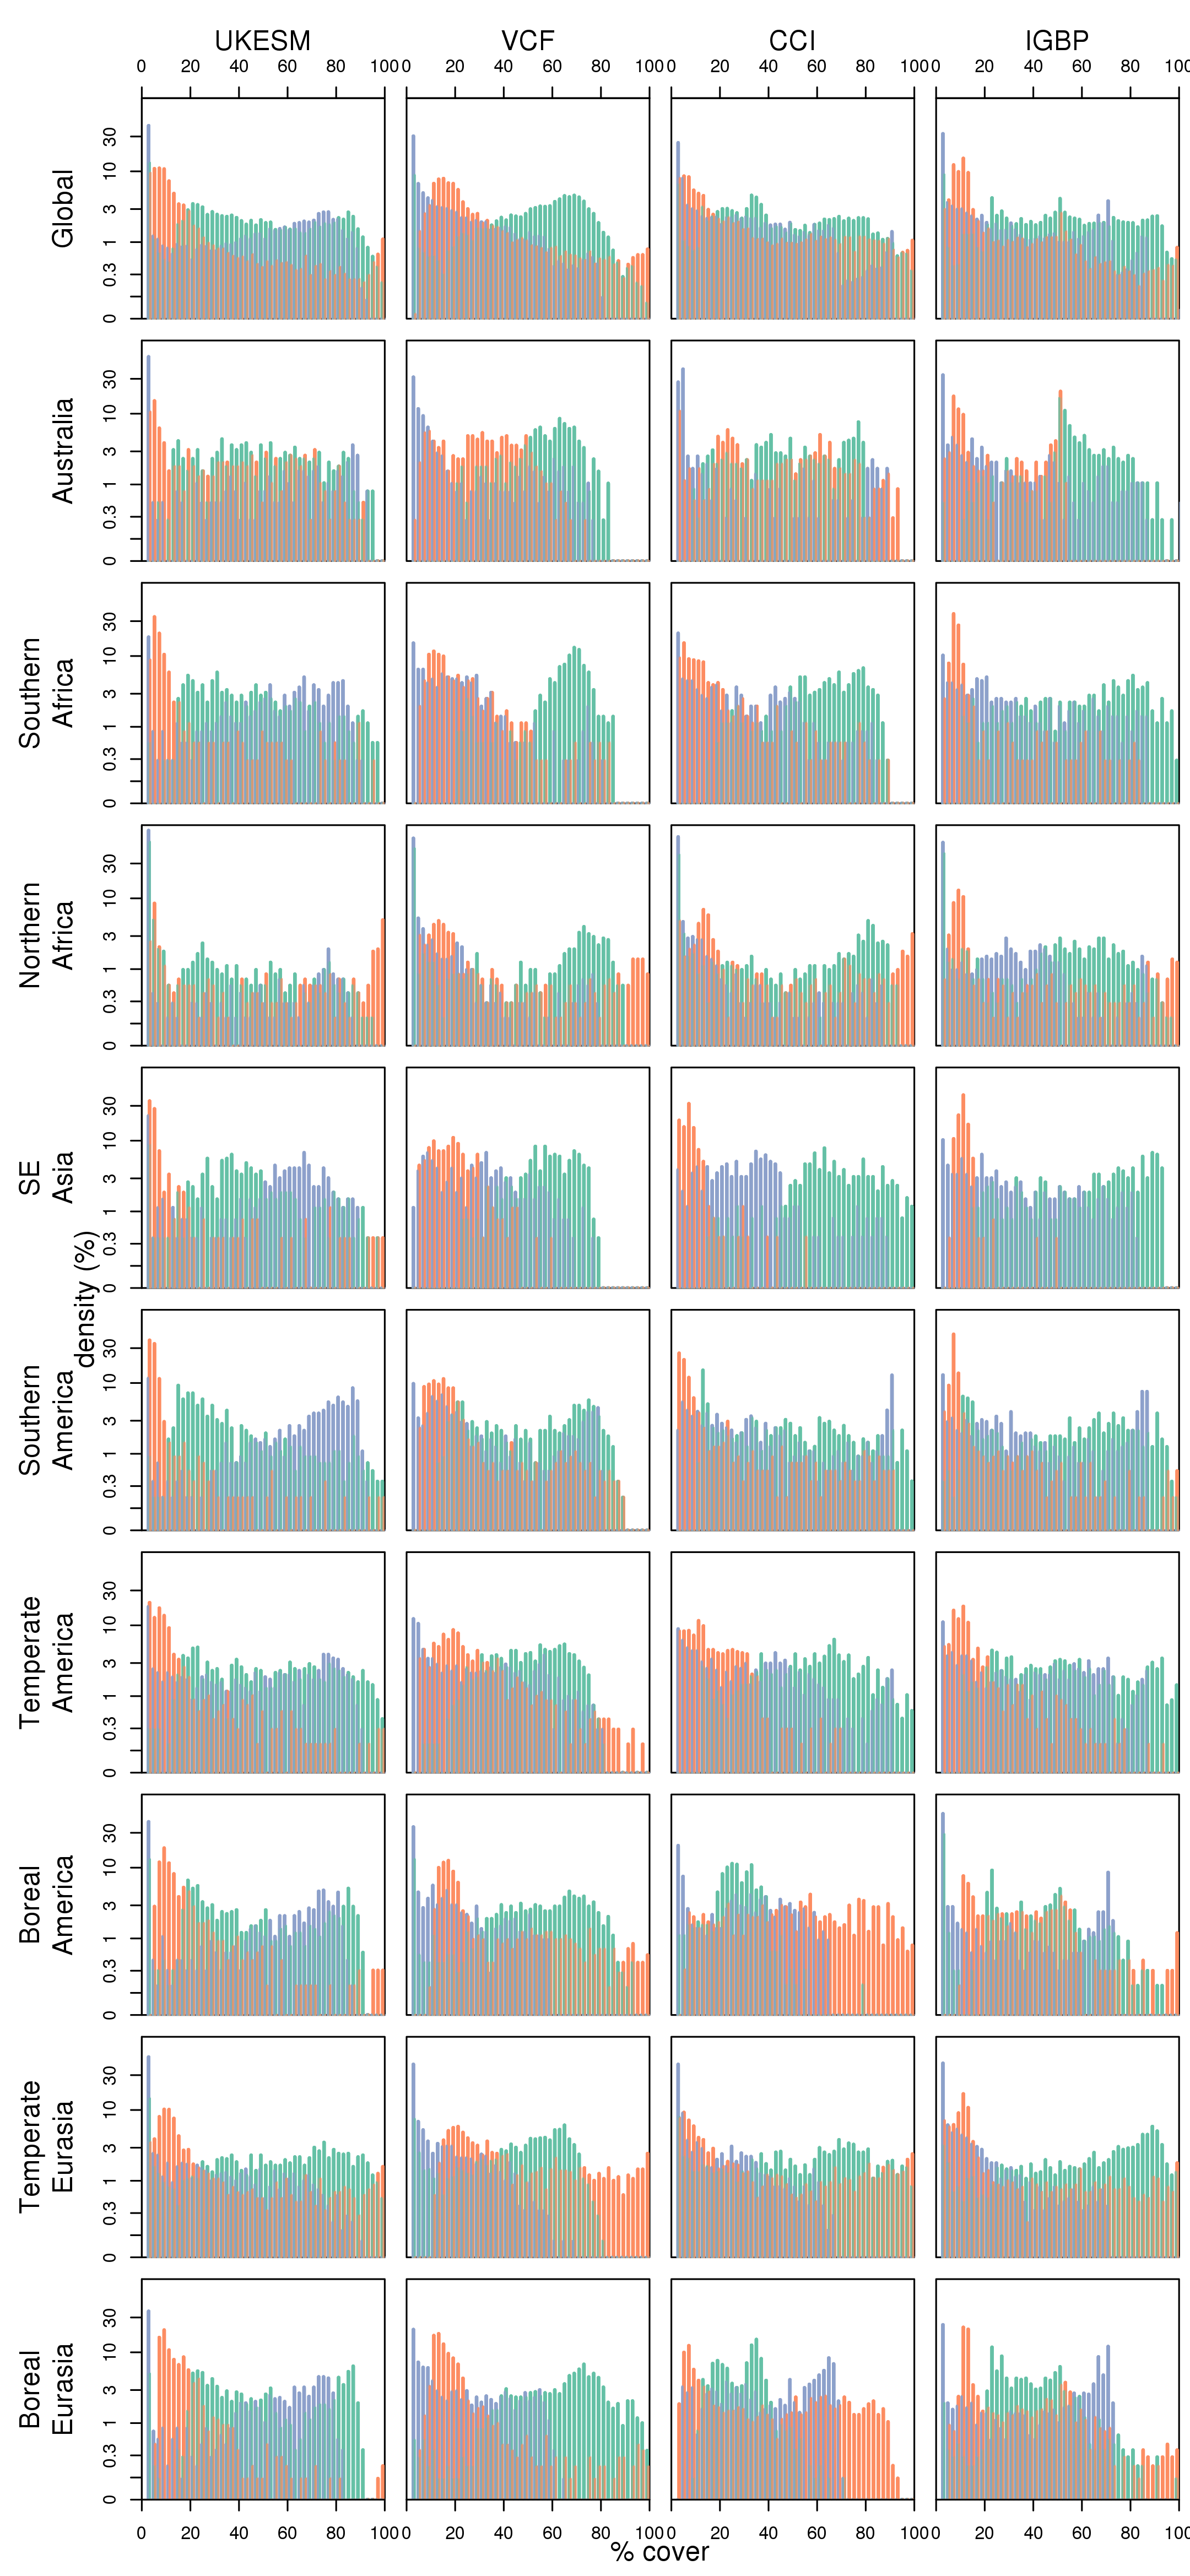
\includegraphics[width=8.3cm]{figs/VegDist/VegDistHist.png}
\caption{Vegetation cover by regions\label{fig:VegDistHist}}
\end{figure}

\begin{figure*}[t]
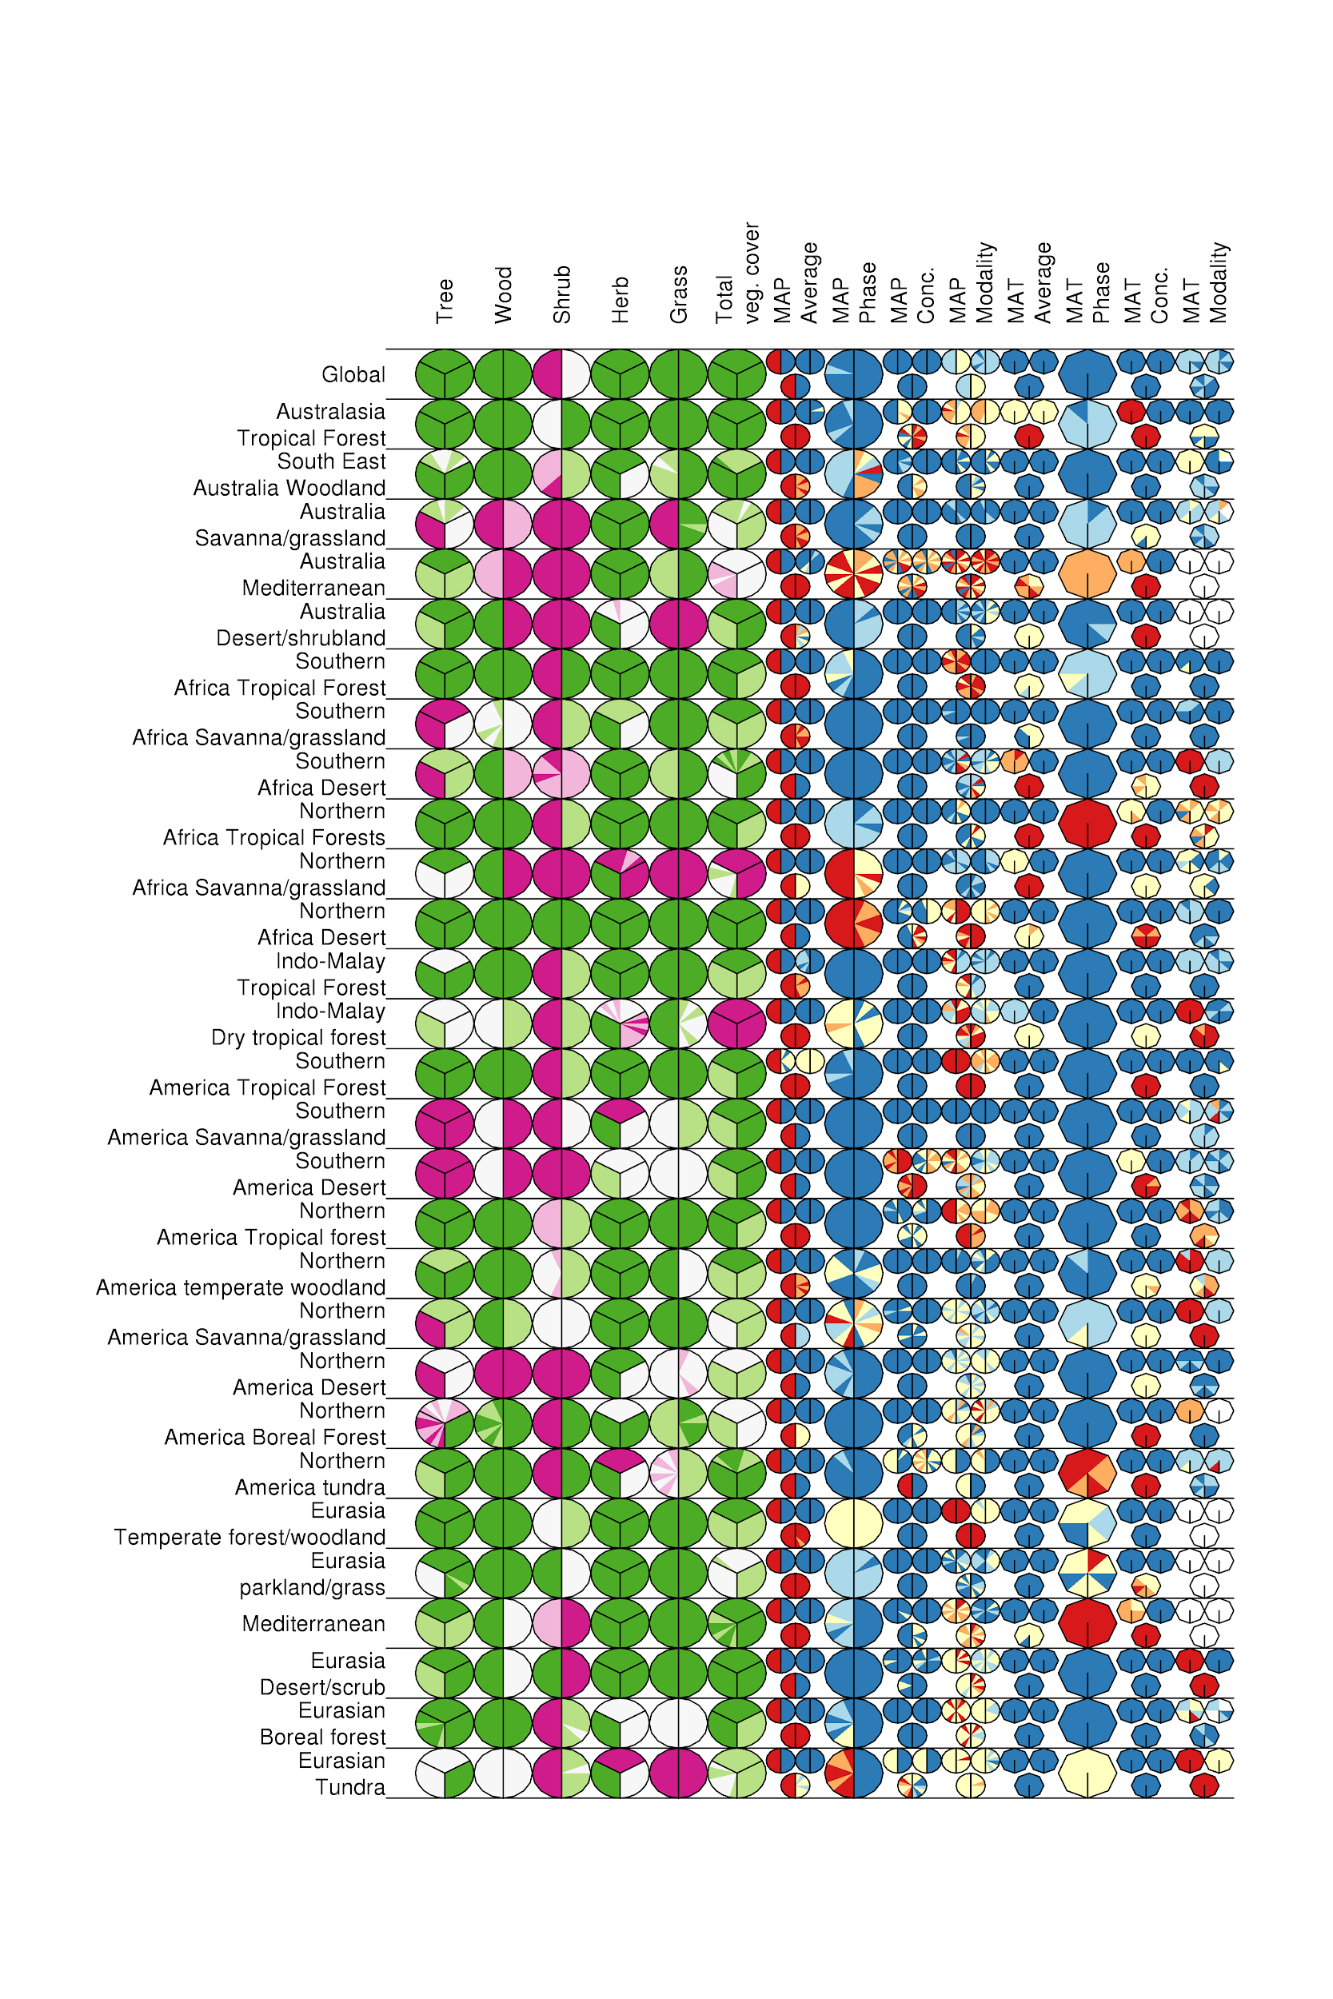
\includegraphics[width=8.3cm]{figs/scores.png}
\caption{needs finishing\label{fig:scores}}
\end{figure*}


\appendixtables   %% needs to be added in front of appendix tables

%% Please add \clearpage between each table and/or figure. Further guidelines on figures and tables can be found below.



\authorcontribution{TEXT} %% this section is mandatory

\competinginterests{TEXT} %% this section is mandatory even if you declare that no competing interests are present

\disclaimer{TEXT} %% optional section

\begin{acknowledgements}
TEXT
\end{acknowledgements}




%% REFERENCES

%% The reference list is compiled as follows:

%\begin{thebibliography}{}
%
%\bibitem[AUTHOR(YEAR)]{LABEL1}
%REFERENCE 1

%\bibitem[AUTHOR(YEAR)]{LABEL2}
%REFERENCE 2
%
%\end{thebibliography}

%% Since the Copernicus LaTeX package includes the BibTeX style file copernicus.bst,
%% authors experienced with BibTeX only have to include the following two lines:
%%
\bibliographystyle{copernicus}
\bibliography{References.bib}
%%
%% URLs and DOIs can be entered in your BibTeX file as:
%%
%% URL = {http://www.xyz.org/~jones/idx_g.htm}
%% DOI = {10.5194/xyz}


%% LITERATURE CITATIONS
%%
%% command                        & example result
%% \citet{jones90}|               & Jones et al. (1990)
%% \citep{jones90}|               & (Jones et al., 1990)
%% \citep{jones90,jones93}|       & (Jones et al., 1990, 1993)
%% \citep[p.~32]{jones90}|        & (Jones et al., 1990, p.~32)
%% \citep[e.g.,][]{jones90}|      & (e.g., Jones et al., 1990)
%% \citep[e.g.,][p.~32]{jones90}| & (e.g., Jones et al., 1990, p.~32)
%% \citeauthor{jones90}|          & Jones et al.
%% \citeyear{jones90}|            & 1990



%% FIGURES

%% When figures and tables are placed at the end of the MS (article in one-column style), please add \clearpage
%% between bibliography and first table and/or figure as well as between each table and/or figure.


%% ONE-COLUMN FIGURES

%%f
%\begin{figure}[t]
%\includegraphics[width=8.3cm]{FILE NAME}
%\caption{TEXT}
%\end{figure}
%
%%% TWO-COLUMN FIGURES
%
%%f
%\begin{figure*}[t]
%\includegraphics[width=12cm]{FILE NAME}
%\caption{TEXT}
%\end{figure*}
%
%
%%% TABLES
%%%
%%% The different columns must be seperated with a & command and should
%%% end with \\ to identify the column brake.
%
%%% ONE-COLUMN TABLE
%
%%t
%\begin{table}[t]
%\caption{TEXT}
%\begin{tabular}{column = lcr}
%\tophline
%
%\middlehline
%
%\bottomhline
%\end{tabular}
%\belowtable{} % Table Footnotes
%\end{table}
%
%%% TWO-COLUMN TABLE
%
%%t
%\begin{table*}[t]
%\caption{TEXT}
%\begin{tabular}{column = lcr}
%\tophline
%
%\middlehline
%
%\bottomhline
%\end{tabular}
%\belowtable{} % Table Footnotes
%\end{table*}
%
% Please add the following required packages to your document preamble:
% \usepackage{multirow}
% \usepackage[table,xcdraw]{xcolor}
% If you use beamer only pass "xcolor=table" option, i.e. \documentclass[xcolor=table]{beamer}

\begin{sidewaystable*}[t]
\caption{Benchmark datasets}
%\begin{tabular}{column = lcr}
%\tophline
%
%\middlehline
%
%\bottomhline
%\end{tabular}
%\belowtable{} % Table Footnotes
%\end{sidewaystable*}
%\begin{table}[]

\begin{tabular}{lllllll}
\textbf{Variable}                  & \textbf{Dataset}                       & \textbf{Type}                & \textbf{Extent} & \textbf{Time period}                                  & \textbf{Comparisons}                                                 & \textbf{Data source}                            \\

                                   & IGBP                                   & Gridded                      & Global          &                                                       &                                                                      &  (Loveland et al., 2000)    \\
                                   & CCI                                    & Gridded                      & Global          &                                                       & \multirow{-2}{*}{Tree, wood, shrub, herb, grass and total veg cover} &  (Poulter et al., 2015)      \\
\multirow{-3}{*}{Vegetation Cover} & VCF                                    & Gridded                      & Global          & 2000-2014                                             & Tree, herb and total veg cover                                       & (Dimiceli and Others, n.d.) \\
Leaf Area Index                    &                                        & Gridded                      & Global          & 2000-2014                                             & Annual average and seasonal                                          &                                                 \\
Carbon                             &                                        &                              &                 &                                                       &                                                                      &                                                 \\
Turnover                           &                                        &                              &                 &                                                       &                                                                      &                                                 \\
                                   & CRUTS4.01                              & Gridded, gauge               & Global          & 2000-2014                                             &                                                                      &                                                 \\
                                   & GPCP2                                  & Gridded, gauge and satellite & Global          & 1982-2008                                             &                                                                      &                                                 \\
\multirow{-3}{*}{Precipitation}    & GPCC                                   & Gridded, gauge               & Global          &                                                       & \multirow{-3}{*}{Annual average and seasonal}                        &                                                 \\
                                   & CMAP                                   & Gridded, gauge and satellite & Global          &                                                       &                                                                      &                                                 \\
Short Wave                         & CERES                                  & Gridded                      & Global          & 1982-2008                                             &                                                                      &                                                 \\
                                   & CRUTS4.01                              & Gridded                      & Global          & 2000-2014                                             & Annual average and seasonal                                          &                                                 \\
                                   & xxx                                    &                              &                 &                                                       &                                                                      &                                                 \\
\multirow{-3}{*}{Air temp}         & GSWP3                                  & Gridded                      &                 &                                                       & Permafrost extent                                                    &                                                 \\
LST                                &                                        &                              &                 &                                                       &                                                                      &                                                 \\
Snow                               &                                        &                              &                 &                                                       &                                                                      &                                                 \\
Albedo                             &                                        &                              &                 &                                                       &                                                                      &                                                 \\
Drought/heatwaves                  &                                        &                              &                 &                                                       &                                                                      &                                                 \\
Wetlands                           & WAD2M                            & Gridded                             &  Global               &   2000-2018                                                    &   Wetland Extent Zonal Mean                                                                  &       (Poulter et al., 2017) (Zhen et al., 2020, submitted)                          \\
River discharge                    & (Dai et al., 2009) & Gauge station                &                 & 1990-2005 used (but 1900-2006 potentially  available) & Mean annual used (but monthly available)                             & (Dai et al., 2009)       
\end{tabular}
%\end{table}
\end{sidewaystable*}

%%% LANDSCAPE TABLE
%
%%t
%\begin{sidewaystable*}[t]
%\caption{TEXT}
%\begin{tabular}{column = lcr}
%\tophline
%
%\middlehline
%
%\bottomhline
%\end{tabular}
%\belowtable{} % Table Footnotes
%\end{sidewaystable*}
%
%
%%% MATHEMATICAL EXPRESSIONS
%
%%% All papers typeset by Copernicus Publications follow the math typesetting regulations
%%% given by the IUPAC Green Book (IUPAC: Quantities, Units and Symbols in Physical Chemistry,
%%% 2nd Edn., Blackwell Science, available at: http://old.iupac.org/publications/books/gbook/green_book_2ed.pdf, 1993).
%%%
%%% Physical quantities/variables are typeset in italic font (t for time, T for Temperature)
%%% Indices which are not defined are typeset in italic font (x, y, z, a, b, c)
%%% Items/objects which are defined are typeset in roman font (Car A, Car B)
%%% Descriptions/specifications which are defined by itself are typeset in roman font (abs, rel, ref, tot, net, ice)
%%% Abbreviations from 2 letters are typeset in roman font (RH, LAI)
%%% Vectors are identified in bold italic font using \vec{x}
%%% Matrices are identified in bold roman font
%%% Multiplication signs are typeset using the LaTeX commands \times (for vector products, grids, and exponential notations) or \cdot
%%% The character * should not be applied as mutliplication sign
%
%
%%% EQUATIONS
%
%%% Single-row equation
%
%\begin{equation}
%
%\end{equation}
%
%%% Multiline equation
%
%\begin{align}
%& 3 + 5 = 8\\
%& 3 + 5 = 8\\
%& 3 + 5 = 8
%\end{align}
%
%
%%% MATRICES
%
%\begin{matrix}
%x & y & z\\
%x & y & z\\
%x & y & z\\
%\end{matrix}
%
%
%%% ALGORITHM
%
%\begin{algorithm}
%\caption{...}
%\label{a1}
%\begin{algorithmic}
%...
%\end{algorithmic}
%\end{algorithm}
%
%
%%% CHEMICAL FORMULAS AND REACTIONS
%
%%% For formulas embedded in the text, please use \chem{}
%
%%% The reaction environment creates labels including the letter R, i.e. (R1), (R2), etc.
%
%\begin{reaction}
%%% \rightarrow should be used for normal (one-way) chemical reactions
%%% \rightleftharpoons should be used for equilibria
%%% \leftrightarrow should be used for resonance structures
%\end{reaction}
%
%
%%% PHYSICAL UNITS
%%%
%%% Please use \unit{} and apply the exponential notation


\end{document}
